\documentclass[12pt]{article}

    \input{preambula_pakiety.tex}
    % ------------------------------------------------------------------------
% USTAWIENIA
% ------------------------------------------------------------------------

% ------------------------------------------------------------------------
%   Kropki po numerach sekcji, podsekcji, itd.
%   Np. 1.2. Tytul podrozdzialu
% ------------------------------------------------------------------------
\makeatletter
    \def\numberline#1{\hb@xt@\@tempdima{#1.\hfil}}                      %kropki w spisie treści
    \renewcommand*\@seccntformat[1]{\csname the#1\endcsname.\enspace}   %kropki w treści dokumentu
\makeatother

% ------------------------------------------------------------------------
%   Numeracja równań, rysunków i tabel
%   Np.: (1.2), gdzie:
%   1 - numer sekcji, 2 - numer równania, rysunku, tabeli
%   Uwaga ogólna: o otoczeniu figure ma być najpierw \caption{}, potem \label{}, inaczej odnośnik nie działa!
% ------------------------------------------------------------------------
\makeatletter
    \@addtoreset{equation}{section} %resetuje licznik po rozpoczęciu nowej sekcji
    \renewcommand{\theequation}{{\thesection}.\@arabic\c@equation} %dodaje kropkę

    \@addtoreset{figure}{section}
    \renewcommand{\thefigure}{{\thesection}.\@arabic\c@figure}

    \@addtoreset{table}{section}
    \renewcommand{\thetable}{{\thesection}.\@arabic\c@table}
\makeatother

% ------------------------------------------------------------------------
% Tablica
% ------------------------------------------------------------------------
\newenvironment{tablica}[3]
{
    \begin{table}[!tb]
    \centering
    \caption[#1]{#2}
    \vskip 9pt
    #3
}{
    \end{table}
}

% ------------------------------------------------------------------------
% Dostosowanie wygl?du pozycji listy \todos, np. zamiast 'p.' jest 'str.'
% ------------------------------------------------------------------------
\renewcommand{\todoitem}[2]{%
    \item \label{todo:\thetodo}%
    \ifx#1\todomark%
        \else\textbf{#1 }%
    \fi%
    (str.~\pageref{todopage:\thetodo})\ #2}
\renewcommand{\todoname}{Do zrobienia...}
\renewcommand{\todomark}{~uzupełnić}

% ------------------------------------------------------------------------
% Definicje
% ------------------------------------------------------------------------
\def\nonumsection#1{%
    \section*{#1}%
    \addcontentsline{toc}{section}{#1}%
    }
\def\nonumsubsection#1{%
    \subsection*{#1}%
    \addcontentsline{toc}{subsection}{#1}%
    }
\reversemarginpar %umieszcza notki po lewej stronie, czyli tam gdzie jest więcej miejsca
\def\notka#1{%
    \marginpar{\footnotesize{#1}}%
    }
\def\mathcal#1{%
    \mathscr{#1}%
    }
\newcommand{\atp}{ATP/EMTP} % Inaczej: \def\atp{ATP/EMTP}

% ------------------------------------------------------------------------
% Inne
% ------------------------------------------------------------------------
\frenchspacing                      %nie pamiętam co to jest, ale używam
%\flushbottom                       %nie pamiętam co to jest, ale nie używam
%\raggedbottom                      %nie pamiętam co to jest, ale nie używam
\hyphenation{ATP/-EMTP}             %dzielenie wyrazu w żądanym miejscu
\setlength{\parskip}{3pt}           %odstęp pomiędzy akapitami
\linespread{1.2}                    %odstęp pomiędzy liniami (interlinia)
\setcounter{tocdepth}{4}            %uwzględnianie w spisie treści czterech poziomów sekcji
\setcounter{secnumdepth}{4}         %numerowanie do czwartego poziomu sekcji włącznie
\titleformat{\paragraph}[hang]      %wygląd nagłówków
{\normalfont\sffamily\bfseries}{\theparagraph}{1em}{}
%\definecolor{niebieski}{rgb}{0.0,0.0,0.5}


    \title{Wykorzystanie silników fizycznych na platformach mobilnych}
    \author{Mateusz Kortas}

    %polecenia zdefiniowane w pakiecie strona_tytulowa.sty
    \uczelnia{POLITECHNIKA GDAŃSKA}
    \instytut{Katedra Fizyki Teoretycznej i Informatyki Kwantowej}
    \promotor{dr. B. Reichel}
    \praca{PRACA MAGISTERSKA}
    \rok{2012}
    %\draft  %comment out for draft
    %koniec poleceń zdefiniowanych przez pakiet strona_tytulowa.sty

    %skorowidz
    %\makeindex
    %koniec skorowidza

\begin{document}
	\sloppy %zakaz wydłużania lini (gdzy nie może złożyć)
	\clubpenalty=10000 %to kara za sierotki
	\widowpenalty=10000 %nie pozostawia wdów
	\brokenpenalty=10000 %nie dieli wyrazów pomiędzy stronami
    \renewcommand{\figurename}{Rysunek}    %musi byc pod \begin{document}, bo w~tym miejscu pakiet 'babel' narzuca swoje ustawienia
    \renewcommand{\tablename}{Tabela}     %j.w.
    \renewcommand{\lstlistingname}{Listing}     %j.w.
    %\renewcommand*{\arraystretch}{1.5}  %zwieksza spacing w macierzach
    \pagenumbering{arabic}              %numeracja stron: rzymska
    \thispagestyle{empty}               %na tej stronie: brak numeru
    \stronatytulowa                     %strona tytułowa tworzona przez pakiet strona_tytulowa.tex

    %podziękowania
    \newpage
    ~   %potrzebne dla \vfill
    \vfill
    {\sffamily
    
    \begin{flushright}
        \begin{tabular}{r}
        Składam serdeczne podziękowania Panu dr Bartoszowi Reichelowi \\
        za poświęcony czas i cenne wskazówki merytoryczne \\
        udzielane na każdym etapie tworzenia pracy.
        \end{tabular}
    \end{flushright}
    }
    \vskip0.5in
    \thispagestyle{empty}
    \newpage
    %koniec podziękowań

    %formatowanie spisu treści i~nagłówków
    \hypersetup{linkcolor=black}
    \renewcommand{\cftbeforesecskip}{8pt}
    \renewcommand{\cftsecafterpnum}{\vskip 8pt}
    \renewcommand{\cftparskip}{3pt}
    \renewcommand{\cfttoctitlefont}{\Large\bfseries\sffamily}
    \renewcommand{\cftsecfont}{\bfseries\sffamily}
    \renewcommand{\cftsubsecfont}{\sffamily}
    \renewcommand{\cftsubsubsecfont}{\sffamily}
    \renewcommand{\cftparafont}{\sffamily}
    %koniec formatowania spisu treści i nagłówków

    \tableofcontents    %spis treści
    \newpage

    \nonumsection{Wykaz ważniejszych skrótów i~oznaczeń}
\suppressfloats[t]

\begin{description}[\setleftmargin{65pt}\setlabelstyle{\bfseries}]
    \leftskip=1cm

	\item[$SDK$]      	Software Development Kit
    \item[$NDK$]      	Native Development Kit
    \item[$JNI$]      	Java Native Interface
    \item[$CDT$]        C++ Development Tools
    \item[$GPU$]		Graphics Processing Unit
    \item[$PPU$]        Physics Processing Unit
    \item[$GPGPU$]      General Purpose processing on Graphics Processing Unit
    \item[$ADT$]        Android Developer Tools
    \item[$JVM$]        Java Virtual Machine
    \item[$DoF$]        Stopnie swobody - Degrees of Freedom
    \item[$FoV$]		Pole widzenia - Field of View
    \item[$CSV$]		Comma Separated Values
\end{description}

    \newpage

    %spis rysunków i tabel
    %format spisu treści dotyczy tylko tych spisów, które są poniżej
    \hypersetup{linkcolor=black}
    \renewcommand{\cftparskip}{3pt}
    \clearpage
    \renewcommand{\cftloftitlefont}{\Large\bfseries\sffamily}
    \listoffigures
    \addcontentsline{toc}{section}{Spis rysunków}
    \newpage
    \renewcommand{\cftlottitlefont}{\Large\bfseries\sffamily}
    \listoftables
    \addcontentsline{toc}{section}{Spis tablic}
    \newpage
    %powrót do czerwonego koloru dla dalszych odnośników (spis literatury, przy włączonym pokazywaniu numerów stron, do których odnoszą się poszczególne pozycje)
    \hypersetup{linkcolor=red}
    %koniec spisu rysunków i~tablic

    %przeniesienie warto sci licznika stron na strony numerowane innym stylem (arabic)
    \newcounter{licznikStron}
    \setcounter{licznikStron}{\value{page}}
    \pagenumbering{arabic}
    \setcounter{page}{\value{licznikStron}}
    %koniec przeniesienia...

    %treść główna dokumentu
    \documentclass[12pt]{article}
\usepackage{polski}
\usepackage[utf8]{inputenc}
\usepackage{amsmath}
\usepackage{anysize}
\usepackage{mathrsfs}   %Różne symbole matematyczne opisane w katalogu ~\doc\latex\comprehensive. Zamienia \mathcal{L} ze zwykłego L na L-transformatę.
\usepackage{eucal}      %Różne symbole matematyczne.
\usepackage{amssymb}    %Różne symbole matematyczne.
\usepackage{amsmath}    %Dodatkowe funkcje matematyczne, np. polecenie \dfac{}{} skladajace ulamek w trybie wystawionym (porównaj $\dfrac{1}{2}$, a $\frac{1}{2}$).
\usepackage{listings}
\lstset
{
  language=C++,                % the language of the code
  % basicstyle=\footnotesize,           % the size of the fonts that are used for the code
  numbers=left,                   % where to put the line-numbers
  numberstyle=\color{gray},  % the style that is used for the line-numbers
  stepnumber=1,                   % the step between two line-numbers. If it's 1, each line 
                                  % will be numbered
  numbersep=3pt,                  % how far the line-numbers are from the code
  backgroundcolor=\color{white},      % choose the background color. You must add \usepackage{color}
  showspaces=false,               % show spaces adding particular underscores
  showstringspaces=false,         % underline spaces within strings
  showtabs=false,                 % show tabs within strings adding particular underscores
  %frame=single,                   % adds a frame around the code
  %rulecolor=\color{black},        % if not set, the frame-color may be changed on line-breaks within not-black text (e.g. commens (green here))
  tabsize=2,                      % sets default tabsize to 2 spaces
  basicstyle=\footnotesize,
  breaklines=true,                % sets automatic line breaking
  breakatwhitespace=false,        % sets if automatic breaks should only happen at whitespace
  xleftmargin=12pt,
                                  % also try caption instead of title
  keywordstyle=\color{blue},          % keyword style
  commentstyle=\color{darkgreen},       % comment style
  stringstyle=\color{red},         % string literal style
  escapeinside={\%*}{*)},            % if you want to add LaTeX within your code
  morekeywords={*,...}               % if you want to add more keywords to the set
}
\usepackage{graphicx}
\usepackage{color}
\usepackage{strona_tytulowa}

\usepackage{etex}	%musi byc przed tikz i pgfplot

%inne
\usepackage[hide]{todo}                     %Wprowadza polecenie \todo{treść}. Opcje pakietu: hide/show. Polecenie \todos ma byc na koncu dokumentu, wszystkie \todo{} po \todos sa ignorowane.
\usepackage{tikz}
\usetikzlibrary{arrows,shapes,automata,backgrounds,petri,calc}
%\usepackage{gnuplottex}
\usepackage[basic,physics]{circ}            %Wprowadza środowisko circuit do rysowania obwodów elektrycznych. Musi byc poniżej pakietow językowych.
\usepackage[sf,bf,outermarks]{titlesec}     %Troszczy się o wygląd tytułów rozdziałów (section, subsection, ...). sf oznacza czcionkę sans serif (typu arial), bf -- bold. U mnie: oddzielna linia dla naglowku paragraph. Patrz tez: tocloft -- lepiej robi format spisu tresci.
\usepackage{indentfirst} %wcina 1 akapit (wg polskiej typogreafii wskazane)
\usepackage{tocloft}                        %Troszczy się o format spisu trsci.
\usepackage{expdlist}    %Zmienia definicję środowiska description, daje większe możliwości wpływu na wygląd listy.
\usepackage{flafter}     %Wprowadza parametr [tb] do polecenia \suppressfloats[t] (polecenie to powoduje nie umieszczanie rysunkow, tabel itp. na stronach, na ktorych jest to polecenie (np. moze byc to stroma z tytulem rozdzialu, ktory chcemy zeby byl u samej gory, a nie np. pod rysunkiem)).
\usepackage{array}       %Ładniej drukuje tabelki (np. daje wiecej miejsca w komorkach -- nie są tak ścieśnione, jak bez tego pakietu).
\usepackage{listings}    %Listingi programow.
\usepackage{subcaption}
\usepackage[format=hang,labelsep=period,labelfont={bf,small},textfont=small]{caption}   %Formatuje podpisy pod rysunkami i tabelami. Parametr 'hang' powoduje wcięcie kolejnych linii podpisu na szerokosc nazwy podpisu, np. 'Rysunek 1.'.
\DeclareCaptionFont{white}{\color{white}}
\DeclareCaptionFormat{listing}{\colorbox{gray}{\parbox{\dimexpr\textwidth-2\fboxsep\relax}{#1#2#3}}}
% ------------------------------------------------------------------------
% USTAWIENIA
% ------------------------------------------------------------------------

% ------------------------------------------------------------------------
%   Kropki po numerach sekcji, podsekcji, itd.
%   Np. 1.2. Tytul podrozdzialu
% ------------------------------------------------------------------------
\makeatletter
    \def\numberline#1{\hb@xt@\@tempdima{#1.\hfil}}                      %kropki w spisie treści
    \renewcommand*\@seccntformat[1]{\csname the#1\endcsname.\enspace}   %kropki w treści dokumentu
\makeatother

% ------------------------------------------------------------------------
%   Numeracja równań, rysunków i tabel
%   Np.: (1.2), gdzie:
%   1 - numer sekcji, 2 - numer równania, rysunku, tabeli
%   Uwaga ogólna: o otoczeniu figure ma być najpierw \caption{}, potem \label{}, inaczej odnośnik nie działa!
% ------------------------------------------------------------------------
\makeatletter
    \@addtoreset{equation}{section} %resetuje licznik po rozpoczęciu nowej sekcji
    \renewcommand{\theequation}{{\thesection}.\@arabic\c@equation} %dodaje kropkę

    \@addtoreset{figure}{section}
    \renewcommand{\thefigure}{{\thesection}.\@arabic\c@figure}

    \@addtoreset{table}{section}
    \renewcommand{\thetable}{{\thesection}.\@arabic\c@table}
\makeatother

% ------------------------------------------------------------------------
% Tablica
% ------------------------------------------------------------------------
\newenvironment{tablica}[3]
{
    \begin{table}[!tb]
    \centering
    \caption[#1]{#2}
    \vskip 9pt
    #3
}{
    \end{table}
}

% ------------------------------------------------------------------------
% Dostosowanie wygl?du pozycji listy \todos, np. zamiast 'p.' jest 'str.'
% ------------------------------------------------------------------------
\renewcommand{\todoitem}[2]{%
    \item \label{todo:\thetodo}%
    \ifx#1\todomark%
        \else\textbf{#1 }%
    \fi%
    (str.~\pageref{todopage:\thetodo})\ #2}
\renewcommand{\todoname}{Do zrobienia...}
\renewcommand{\todomark}{~uzupełnić}

% ------------------------------------------------------------------------
% Definicje
% ------------------------------------------------------------------------
\def\nonumsection#1{%
    \section*{#1}%
    \addcontentsline{toc}{section}{#1}%
    }
\def\nonumsubsection#1{%
    \subsection*{#1}%
    \addcontentsline{toc}{subsection}{#1}%
    }
\reversemarginpar %umieszcza notki po lewej stronie, czyli tam gdzie jest więcej miejsca
\def\notka#1{%
    \marginpar{\footnotesize{#1}}%
    }
\def\mathcal#1{%
    \mathscr{#1}%
    }
\newcommand{\atp}{ATP/EMTP} % Inaczej: \def\atp{ATP/EMTP}

% ------------------------------------------------------------------------
% Inne
% ------------------------------------------------------------------------
\frenchspacing                      %nie pamiętam co to jest, ale używam
%\flushbottom                       %nie pamiętam co to jest, ale nie używam
%\raggedbottom                      %nie pamiętam co to jest, ale nie używam
\hyphenation{ATP/-EMTP}             %dzielenie wyrazu w żądanym miejscu
\setlength{\parskip}{3pt}           %odstęp pomiędzy akapitami
\linespread{1.2}                    %odstęp pomiędzy liniami (interlinia)
\setcounter{tocdepth}{4}            %uwzględnianie w spisie treści czterech poziomów sekcji
\setcounter{secnumdepth}{4}         %numerowanie do czwartego poziomu sekcji włącznie
\titleformat{\paragraph}[hang]      %wygląd nagłówków
{\normalfont\sffamily\bfseries}{\theparagraph}{1em}{}
%\definecolor{niebieski}{rgb}{0.0,0.0,0.5}

\title{Wykorzystanie silników fizycznych na platformach mobilnych}
\author{Mateusz Kortas}
\date{12.05.2012}
\uczelnia{POLITECHNIKA GDAŃSKA}
    \instytut{Katedra Fizyki Teoretycznej i Informatyki Kwantowej}
    \promotor{dr. B. Reichel}
    \praca{PRACA MAGISTERSKA}
    \rok{2012}
\begin{document}
	\sloppy %zakaz wydłużania lini (gdzy nie może złożyć)
	\clubpenalty=10000 %to kara za sierotki
	\widowpenalty=10000 %nie pozostawia wdów
	\brokenpenalty=10000 %nie dieli wyrazów pomiędzy stronami
    \renewcommand{\figurename}{Rysunek}    %musi byc pod \begin{document}, bo w~tym miejscu pakiet 'babel' narzuca swoje ustawienia
    \renewcommand{\tablename}{Tabela}     %j.w.
    \renewcommand{\lstlistingname}{Listing}     %j.w.
    %\renewcommand*{\arraystretch}{1.5}  %zwieksza spacing w macierzach
    \pagenumbering{arabic}              %numeracja stron: rzymska
    \thispagestyle{empty}               %na tej stronie: brak numeru
    \stronatytulowa                     %strona tytułowa tworzona przez pakiet strona_tytulowa.tex

    %podziękowania
    \newpage
    ~   %potrzebne dla \vfill
    \vfill
    {\sffamily
    
    \begin{flushright}
        \begin{tabular}{r}
        Składam serdeczne podziękowania Panu dr Bartoszowi Reichelowi \\
        za poświęcony czas i cenne wskazówki merytoryczne \\
        udzielane na każdym etapie tworzenia pracy.
        \end{tabular}
    \end{flushright}
    }
    \vskip0.5in
    \thispagestyle{empty}
    \newpage
    %koniec podziękowań

    %formatowanie spisu treści i~nagłówków
    \hypersetup{linkcolor=black}
    \renewcommand{\cftbeforesecskip}{8pt}
    \renewcommand{\cftsecafterpnum}{\vskip 8pt}
    \renewcommand{\cftparskip}{3pt}
    \renewcommand{\cfttoctitlefont}{\Large\bfseries\sffamily}
    \renewcommand{\cftsecfont}{\bfseries\sffamily}
    \renewcommand{\cftsubsecfont}{\sffamily}
    \renewcommand{\cftsubsubsecfont}{\sffamily}
    \renewcommand{\cftparafont}{\sffamily}
    %koniec formatowania spisu treści i nagłówków

    \tableofcontents    %spis treści
    \newpage

    \nonumsection{Wykaz ważniejszych skrótów i~oznaczeń}
\suppressfloats[t]

\begin{description}[\setleftmargin{65pt}\setlabelstyle{\bfseries}]
    \leftskip=1cm

	\item[$SDK$]      	Software Development Kit
    \item[$NDK$]      	Native Development Kit
    \item[$JNI$]      	Java Native Interface
    \item[$CDT$]        C++ Development Tools
    \item[$GPU$]		Graphics Processing Unit
    \item[$PPU$]        Physics Processing Unit
    \item[$GPGPU$]      General Purpose processing on Graphics Processing Unit
    \item[$ADT$]        Android Developer Tools
    \item[$JVM$]        Java Virtual Machine
    \item[$DoF$]        Stopnie swobody - Degrees of Freedom
    \item[$FoV$]		Pole widzenia - Field of View
    \item[$CSV$]		Comma Separated Values
\end{description}

    \newpage

    %spis rysunków i tabel
    %format spisu treści dotyczy tylko tych spisów, które są poniżej
    \hypersetup{linkcolor=black}
    \renewcommand{\cftparskip}{3pt}
    \clearpage
    \renewcommand{\cftloftitlefont}{\Large\bfseries\sffamily}
    \listoffigures
    \addcontentsline{toc}{section}{Spis rysunków}
    \newpage
    \renewcommand{\cftlottitlefont}{\Large\bfseries\sffamily}
    \listoftables
    \addcontentsline{toc}{section}{Spis tablic}
    \newpage
    %powrót do czerwonego koloru dla dalszych odnośników (spis literatury, przy włączonym pokazywaniu numerów stron, do których odnoszą się poszczególne pozycje)
    \hypersetup{linkcolor=red}
    %koniec spisu rysunków i~tablic

    %przeniesienie warto sci licznika stron na strony numerowane innym stylem (arabic)
    \newcounter{licznikStron}
    \setcounter{licznikStron}{\value{page}}
    \pagenumbering{arabic}
    \setcounter{page}{\value{licznikStron}}
    %koniec przeniesienia...

    %treść główna dokumentu
      \section{Wstęp}\label{sec:wstep}
Od początku swojego istnienia komputery i ich moc obliczeniowa były
używane do rozwiązywania problemów fizycznych. Podczas II Wojny Światowej, ENIAC
- pierwszy elektroniczny komputer, był wykorzystywany przez armię Stanów Zjednoczonych do
przewidywania torów lotu pocisków balistycznych (uwzględniając m in. ich masę,
kąt wystrzelenia czy prędkość wiatru). W latach osiemdziesiątych superkomputery
były używane do oblicznaia dynamiki płynów, gdzie poszczególne cząstki były
reprezentowane przez wektory sił, które oddziaływując ze sobą symulowały
cyrkulację cieczy. Aby zwiększyć wydajność tej operacji zostały zaprojektowane
specjalne procesory wektorowe wykonujące operacje na wielu zmiennych
równocześnie. Współcześnie komputerowe wspomaganie obliczeń fizycznych jest
używane w wielu dziedzinach: m in. przez meteorologów do przewidywania zmian
warunków pogodowych, przetwarzania danych tuneli aerodynamicznych w lotnictwie,
czy doborze proporcji materiałów podczas projektowania produktów. Testowanie
przy pomocy symulacji komputerowych jest o wiele tańsze i bezpieczniejsze. Rosnące
zapotrzebowanie na wspomaganie obliczeń fizycznych spowodowało powstanie pojęcia
silnika fizycznego.
  \subsection{Czym jest silnik fizyczny?}\label{subsec:czymJestSilnik}
Silnik fizyczny to rodzaj oprogramowania komputerowego umożliwiającego
przybliżoną symulację pewnych systemów fizycznych jak np. dynamika bryły
sztywnej (w tym wykrywanie kolizji), ciał miękkich i płynów. Przeznaczony jest
do użytku w takich dziedzinach jak: grafika komputerowa, przemysł gier wideo czy
kinematografia. Czasem mianem silnika fizycznego jest również bardziej ogólnie
określane jakiegokolwiek oprogramowania symulującego zachowanie dowolnego
układu w sensie fizycznym.\\
Silniki fizyczne generalnie dzieli się na dwie klasy:\\
\textbf{Wysokoprecyzyjne} (\emph{high-precision}) - lub laboratoryjne.
Pochłaniają one całą (lub większość) mocy obliczeniowej platformy na której
działają aby wyniki ich obliczeń były jak najbardziej zgodne z rzeczywistymi.
Zwykle wykorzystywane są w przemyśle filmowym, prerenderowanych animacjach lub
laboratoriach do celów naukowych czy analiz technicznych. Najpopularniejszymi
dostępnymi publicznie wysokoprecyzyjnymi silnikami są:\\
- VisSim - stworzony przez Visual Solutions silnik fizyczny wykorzystujący
diagramy blokowe\\
- Working Model - komercyjny projekt wykorzystywany do wspomagania projektowania
konstrukcji inżynierskich.\\
\textbf{Wysokowydajnościowe} (\emph{high-performance})
- zwane również silnikami działającymi w czasie rzeczywistym (\emph{real-time
physics engines}), czy po prostu silnikami do gier wideo (\emph{video game
physics engines}). Są stosowane w przypadkach gdy od dokładności symulacji
ważniejszy jest krótki czas otrzymywania wyników, czyli w grach, czy
prezentowanych na żywo symulacjach. Nie wykorzystują one zasobów platformy w
takim stopniu co siniki wysokoprecyzyjne, więc mogą one działać na niemal każdym
sprzęcie, równocześnie obsługując np. rendering. Najpopularniejsze silniki
wysokowydajnościowe to:\\
komercyjne:\\
- Havok\\
- PhysX\\
- Vortex\\
niekomercyjne (\emph{open-source}):\\
- Bullet\\
- Box2D - silnik do symulacji dwuwymiarowych\\
- Newton Game Dynamics\\
- ODE (\emph{Open Dynamics Engine})\\
- PAL (\emph{Physics Abstraction Layer}) - API uwspólniające obsługę kilku
innych silników fizycznych\\

Pojęcie silnika fizycznego nie musi oznaczać tylko oprogramowania. W celu
zwiększenia wydajności symulacji fizycznych na osobistych platformach w 2006
roku narodziła się koncepcja sprzętowego wspomagania obliczeń, tak jak miało to
miejsce z renderingiem i kartami graficznymi. Firma Ageia opracowała PhysX -
pierwszy procesor PPU (\emph{Physics Processing Unit}). PhysX PPU posiadało
możliwość sprzętowego obliczania takich operacji jak dynamika bryły sztywnej, dynamika
ciałą miękkiego, detekcja kolizji, dynamika płynów, symulacja zachowania
elementów ubrań i włosów, analiza przy pomocy metody elementów skończonych.
Podczas demonstracji specjalnie napisanego dema na targach Consumer Electronics
Show 2006 komputer wyposażony w jednostkę PPU odtwarzał symulację z prędkością
30 fps, zaś tak samo skonfigurowana platforma bez wspomagania odtwarzała to samo
demo z prędkością 6 fps. Mimo wszystko koncepcja PPU nie osiągnęła sukcesu. Z
karty PhysX korzysta jedynie kilka gier. W 2008 roku udziały w firmie Ageia
zostały wykupione przez producenta kart graficznych GeForce - Nvidię. Firma
Nvidia wypuściła sterowniki pozwalające obsłużyć API PhysX na kartach GeForce,
tym samym PhysX już jako samo oprogramowanie stał się pierwszym silnikiem
fizycznym korzystającym ze sprzętowego wspomagania. Dało to również początek
koncepcji GPGPU (\emph{General Purpose processing on Graphics Processing Unit}),
czyli wykorzystywania mocy obliczeniowej kart graficznych do obliczeń związanych
z symulacjami fizycznymi. Firma AMD - producent kart Radeon, również oferuje
wsparcie dla tej technologii.

Pomimo swojej niewątpliwej przydatności silniki fizyczne posiadają również swoje
ograniczenia. Najważniejszym z nich jest skończona precyzja przeliczanych
wartości właściwa dla urządzeń cyfrowych. Jeśli precyzja jest niewystarczająca,
pozornie niewielkie błędy wynikające z zaokrąglania wyników mogą drastycznie
zmienić przebieg symulacji. Błędy są widoczne zwłaszcza w przypadkach gdy dwa
swobodne ciała oddziałują ze sobą z przemieszczeniem jednostkowym wymagającym
większej precyzji obliczeń niż silnik jest w stanie zaoferować. Zaobserwować
można wtedy nienaturalne ``trzęsienie się'' ciała. Można ten błąd wyeliminować
zwiększając precyzję obliczeń, jednak odbędzie się to kosztem mocy obliczeniowej
platformy.

\subsection{Cele projektu.}\label{subsec:celeProjektu}
Celami projektu są:\\

\textbf{Uruchomienie silnika fizycznego na mobilnej platformie Android.}\\
Istnieje wiele silników fizycznych dedykowanych na platformy
stacjonarne (głównie procesory firmy Intel). Silnik PhysX od wersji 3.0
posiada wsparcie dla platformy Android jednak do dziś nie istnieje żadne
oficjalne wsparcie open-source'owego silnika dla mobilnych platform. Ponieważ
kod źródłowy silnika Bullet jest ogólnie dostępny, możliwa jest jego kompilacja
na platformę ARM (najczęściej stosowane procesory w urządzeniach mobilnych).
Celem tej częsci pracy będzie sprawdzenie jakie ewentualne trudności może nieść
za sobą ta kompilacja. W celu ułatwienia tworzenia symulacji w silniku Bullet
zostanie stworzone proste obudowanie (\emph{wrapper}) dla języka Java.\\

\textbf{Wykorzystanie możliwości platformy mobilnej pod kątem symulacji
fizycznych.}\\ Smartfony i tablety posiadają kilka możliwości
najczęściej niedostępnych dla platform stacjonarnych (np. akcelerometry czy
ekrany dotykowe). Można je wykorzystać do uatrakcyjnienia symulacji, co
będzie celem tej części pracy.\\

\textbf{Ocena przydatności silnika w symulacjach fizycznych.}\\ Badany
silnik uruchomiony zostanie na platformie mobilnej, których to moc obliczeniowa
nie jest zwykle szczególnie wyskoa. Przez to wybrany silnik - Bullet nie jest
wysokoprecyzyjnym silnikiem fizycznym i nie można się spodziewać wyników
obliczeń bardzo zgodnych z rzeczywistością. Można jednak sprawdzić w jakich
warunkach symulacje będą wykonywane najdokładniej.

\newpage
\section{Wykorzystane technologie.}
W projekcie zostały wykorzystana następujące technologie:

\subsection{Android OS}
Bazujący na jądrze Linux system operacyjny zaprojektowany z myślą o
urządzeniach mobilnych z ekranami dotykowymi, takimi jak smartfony i tablety.
Początkowo tworzony przez Android Inc., później prawa do niego zostały wykupione
przez firmę Google. Kod źródłowy systemu jest ogólnodostępny na licencji Apache. 
Obecnie jest to najpopularniejszy system operacyjny na urządzenia mobilne.
Standardowo jest on instalowany na urządzeniach takich firm jak HTC, Motorola,
Samsung czy Sony Ericsson. Za sprawą wsparcia community, powstaje coraz większa
ilość aplikacji które są dystrybuowane za pośrednictwem uruchomionej przez
Google usługi Google Play (odpowiednik App Marketu na urządzenia firmy Apple).

\subsection{Android SDK}
Android Software Development Kit to zestaw narzędzi deweloperskich służących do
tworzenia Aplikacji na platformę Android. W jeg oskład wchodzą debugger,
biblioteki, emulator oparty na QEMU, dokumentacja, przykłądowy kod oraz
tutoriale. Obecnie wspierane platformy to Linux, Mac OS X 10.5.8 lub nowszy,
Windows XP lub nowszy. Oficjalnym wspieranym środowiskiem programistycznym jest
Eclipse za pośrednictwem wtyczki ADT (\emph{Android Developer Tolls}). Aplikacje
są zwykle pisane w języku Java, jednakże Android nie posiada oficjalnej
implementacji JVM. Zamiast tego na potrzeby systemu powstała specjalna
wirtualna maszayna - Dalvik, która została zprojektowana z myślą o większej
oszczędności energii, czasu procesora i pamięci.

\subsection{Silnik fizyczny Bullet}
Bullet Physics jest obecnie najpopularniejszym darmowym, wysokowydajnościowym
silnikiem fizycznym z otwartym źródłem. Jest szeroko wykorzystywany w grach
wideo (m in. Grand Theft Auto 4, Gravitronix, Red Dead Redemption) jak i
mimo bycia sklasyfikowanym jako wysokowydajnościowy silnik, również w
kinematografii (2012, Shrek, Sherlock Holmes). Bullet jest również domyślnie
używanym silnikiem fizycznym ta takich projektach jak program graficzny
Blender czy silnik gier 3d OGRE.

\subsection{Android NDK}
Biblioteki napisane w kodzie natywnym (C/C++) mogą być kompilowane na platformę
ARM lub x86 i zainstalowane na urządzeniu używająć Android NDK (\emph{Native
Development Kit}). Natywne biblioteki mogą być uruchomione przez maszynę
wirtualną Dalvik używając metody \emph{System.LoadLibrary}. W przeciwieństwie do
Android SDK który bazuje na pluginach do Eclipsa, NDK jest zestawem narzędzi
wywoływanych z wiersza polecenia. Każde zbudowanie projektu musi więc odbyć się
ręcznie. Możliwe jest jednak skonfigurowanie środowiska Eclipse aby kod natywny
był kompilowany automatycznie podczas kompilacji całego projektu (zostało to
opisane w sekcji \ref{sec:autoNDK}). Dostęp do natywnych funkcji z poziomu
języka Java otrzymuje się poprzez JNI (\emph{Java Native Interface}). W tym
projekcie Android NDK będzie wykorzystane do kompilacji kodu biblioteki Bullet
na platformę ARM, oraz wywoływanie jej funkcji przez integrację z kodem
napisanym w języku Java.

\subsection{OpenGL ES}
To podzbiór graficznego API - OpenGL. Zostało zaprojektowane specjalnie na
potrzeby mobilnych urządzeń. Charakteryzuje się zbiorczym przetwarzaniem
danych, czyli do urządzenia graficznego przekazywane są całe bloki pamięci w
przeciwieństwie do charakterystycznych dla OpenGL pojedynczych wywołań. Jego
wersja 3.0 jest obsługiwana przez systemy Android od wersji 2.2.

\newpage
\section{Podstawowe koncepcje silników fizycznych.}
Ponieważ silniki fizyczne są jedynie symulacją, nie można za ich pomocą dokonać
dokładnego odwzorowania rzeczywistości. Dlatego w ich rozwiązaniach użyto
rozmaitych uproszczeń. W tej sekcji zostaną wymienione niektóre z nich.

\subsection{Wykrywanie kolizji}
Podstawowoym problemem każdego silnika fizycznego jest wykrywanie kolizji między
dwoma obiektami. W zależności od tego czy celem jest uzyskanie wysokiej precyzji
czy wydajności symulacji, do tego celu powstało kilka różnych technik.

\subsubsection{Kształty proste (bounding box)}
Metoda polega na wpisaniu porównywanego obiektu najprostszą do sprawdzenia
kolizji bryłę, jak kula czy prostopadłościan. Zbadanie wystąpienia kolizji
między dwoma obiektami ogranicza się wtedy do sprawdzenia kilku prostych
warunków (jak np. dla kul sprawdzenie czy odległość między środkami jest
mniejsza od sumy ich promieni). Metoda ta choć szybka ma bardzo niską
dokładność. Udoskonaleniem tej techniki może być użycie kilku prostych kształtów
do opisania jednego obiektu.

\begin{figure}
\centering
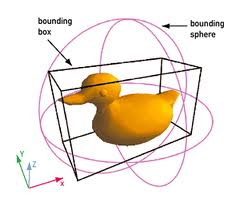
\includegraphics[scale=0.5]{./img/boundingBox.jpg}
\caption{Skomplikowana bryła wpisana w kształt prosty. Źródło:
http://www.tcs.fudan.edu.cn}
\label{fig:bbox}
\end{figure}

\subsubsection{Otoczka wypłukła (convex hull)}
Większość wysokowydajnościowych silników fizycznych operuje na modelach
złożonych z wielokątów (\emph{polygons}). Badając kolizje każdego z nich między
dwoma obiektami w takim przypadku to najdokładniejsza technika, jednak również
najbardziej czasochłonna. Opracowanie techniki zminiejszającej ilość wielokątów
przy zachowaniu ogólnego kształtu bryły początkowej pozwoliłoby na znaczne
przyspieszenie obliczeń. Do tego celu w silnikach fizycznych posłużono się
pojęciem w matematyce zwanym otoczką wypłukłą. \\
Otoczka wypłukła jest definiowana jako najmnieszy spójny zbiór punktów
zawieracjący wszyskie punkty z danego zbioru P. Jednocześnie każdy odicnek
poprowadzony między dwoma dowolnymi punktami ze zbioru P zawiera się również w
otoczce wypłukłej (definicja wypłukłości). Stworzony przy pomocy tego działania
model o zredukowanej ilości wielokątów jest używany do wykrycia kolizji
poszczególnych wielokątów zamiast modelu używanego do wyświetlania. Użycie tej
metody znacznie przyśpiesza obliczenia przy zachowaniu większej dokładności od
metody kształtów prostych. Dokładnośc ta jest jednak wciąż ograniczona. Na
przykład wystrzelony pocisk nie będzie mógł przelecieć przez ucho kubka,
ponieważ dziura w kubku również wchodzi w skład bryły otoczki.

\begin{figure}
\centering

\includegraphics[scale=0.5]{./img/convexhull.png}
\caption{Przykład wyodrębnienia otoczki wypłukłej dla dwuwymiarowego zbioru
punktów. Źródło: http://www.evanjones.ca/convexhulls.html}
\label{fig:convexhull}
\end{figure}

\subsubsection{Metoda elementów skończonych}
Odmiennym podejściem do testowania kolizji poszczególnych wielokątów i
stosowania otoczek wypłukłych stanowi użycie metody elementów skończonych.
Metoda ta jest bardziej zaawanasowanym przypadkiem wariantu z użyciem kształtów
prostych. Obiekt zostaje podzielony na wiele elementów o określonych wcześniej
kształtach. Dzięki temu w odróżnieniu od omówionych wcześniej metod możliwe jest
symulowanie oddziaływań również we wnętrzu rozpatrywanych obiektów, a nie tylko
na ich powierzchni. Co więcej, elementy z których zbudowane jest rozpatrywane
ciało mogą być również charakteryzowane szeregiem odrębnych właściwych dla
siebie parametrów (jak temperatura). Elementy te mogą również się przemieszczać
względem siebie zgodnie z zasadami odkształcenia, dzięki czemu symulowane ciała
nie ograniczają się tylko brył sztywnych jak miało to miejsce w poprzednich
metodach. Niestety, ze względu na znacznie większe zapotrzebowanie na moc
obliczeniową, metoda ta jest wykorzystywana niemal wyłącznie w silnikach
wysokoprecyzyjnych. Silniki wysokowydajnościowe jak Bullet i Havok wykorzystują
również uproszczony wariant tej metody do symulacji zachowań ciał miękkich i płynów.

\begin{figure}
\centering
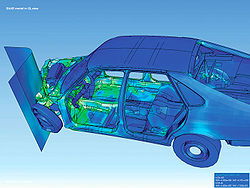
\includegraphics[scale=1]{./img/finiteElementApplication.jpg}
\caption{Przykład zastosowania metody elementów skończonych dla symulacji
rozbijającego się samochodu Źródło:
http://en.wikipedia.org/wiki/Finite\_element}
\label{fig:finiteElementApplication}
\end{figure}

\subsubsection{Wykrywanie kolizji w silniku Bullet}
W silniku Bullet wykrywanie kolizji odbywa się dwufazowo. Każde przetwarzanie
ramki zaczyna się od ``fazy szerokiej'' (\emph{broadphase}), analizując po kolei
wszystkie możliwe pary jakie mogą dokonać zderzenia metodą kształtów prostych.
Następnie każda z par któta przeszła poprzedni test jest analizowana przez
dyspozytor (\emph{dispatcher}) pod względem zderzenia odpowiednim algorytmem (w
zależności od tego czy np. rozpatrywane jest zderzenie bryły zdefinowanej przez
otoczkę wypłukłą czy kształt prosty). W omawianym projekcie zastosowane są
tylko obiekty korzystające z kształtów prostych.

\subsection{Progi ruchu}
W prawdziwym świecie zasady fizyki są zawsze aktywne. Nawet w ciałach
pozostających w spoczynku ich cząstki poruszają się na wskutek ruchów Browna.
Dla wysokowydajnościowego silnika fizycznego taka ciągła bezwarunkowa analiza
ruchu jest niepotrzebnym zużyciem mocy obliczeniowej procesora, co może
doprowadzić do spadku płynności animacji. Dlatego silniki te mogą ``zamrozić''
dane ciało (nie wykonywać obliczeń związanych z jego ruchem) jeśli wartość jego
prędkości nie przekracza określonego progu - zwanego progiem
ruchu (\emph{motion threshold}). Dane ciało może zostać ``odmrożone'' jeśli
zostanie zmuszone do ruchu przez inne ciało lub siłę. W silniku fizycznym Bullet
istnieje możliwość ustalenia wartości progu ruchu indywidualnie dla każdego
ciała.

%\subsection{Oddziaływania dynamiczne}
%\emph{TODO: penalty methods, constraints(warunki), impulses}

\newpage
\section{Wykorzystanie Android NDK jako obudowania dla silnika Bullet}
Aby ułatwić tworzenie testowych scen zostało stworzone obudowanie obiektów
pozwalające korzystać z możliwości sinika Bullet z poziomu języka Java. Dzięki
temu proces tworzenia scen testowych zostaje skrócony oraz możliwe jest
debugowanie kodu w Eclipse IDE.

\subsection{Konfiguracja Android NDK w środowisku Eclipse}\label{sec:autoNDK}
% [source]http://mhandroid.wordpress.com/2011/01/23/using-eclipse-for-android-cc-development/
Ponieważ w przeciwieństwie do Android SDK, dla NDK nie istnieje żadna
oficjalna wtyczka automatyzująca kompilację natywnych bibliotek konieczna jest
kompilacja ręczna z wiersza poleceń. Możliwe jest jednak skonfigurowanie
środowiska Eclipse w celu integracji z NDK.
  
Aby utworzyć projekt Androida z
możliwością edycji i kompilacji bibliotek natywnych należy: \\
1. Zainstalować środowisko Eclipse (i doinstalować do niego wtyczkę
\emph{ADT}).\\
2. Pobrać kolejno \emph{Android SDK} i \emph{NDK}. W celu ułatwienia edycji
plików żródłowych w języku C++ warto również zainstalować wtyczkę 
\emph{CDT}(C++ Development Tools). Potrzebny będzie rónież kod żródłowy
biblioteki Bullet. Dodatki w eclipse instaluje się przez Help $ \rightarrow $
Install  new software\ldots , wpisując adres
http://download.eclipse.org/releases/galileo (lub zamisat galileo wpisać nazwę
swojej wersji Eclipse).
  
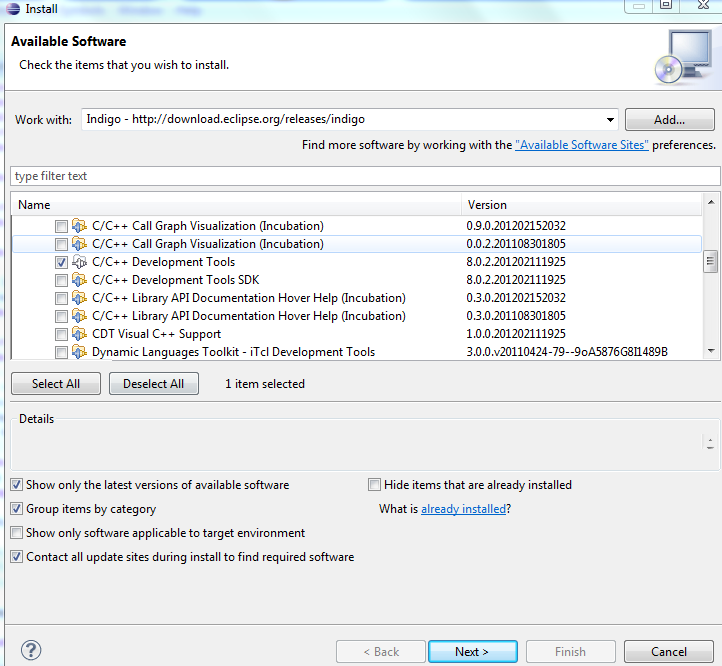
\includegraphics[width=\textwidth]{./img/CDT.png}
3. Utworzyć nowy standardowy projekt aplikacji na system Android.\\
4. Do projektu dodać folder \emph{jni} gdzie przechowywany będzie kod źródłowy
w języku C++. Skopiować do niego foldery z kodu źródłowego biblioteki
Bullet (będą potrzebne biblioteki \emph{BulletCollision},
\emph{BulletDynamics} i \emph{LinearMath}, a także pliki \emph{btBulletCollisionCommon.h},
\emph{btBulletDynamicsCommon.h}, \emph{Bullet-C-Api.h}).
  
\begin{center}
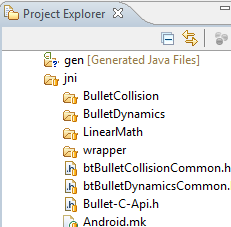
\includegraphics{./img/bulletFoldery.png}
\end{center}
  
5. Umieścić w folderze plik \emph{Android.mk} . Zawiera on informacje jak
powinien być zbudowany projekt w kodzie natywnym. Do tego pliku należy
dodać informacje o plikach źródłowych biblioteki Bullet. Zawartość pliku
\emph{Android.mk} znajduje się w załączniku \ref{att:Androidmk}.
  
  6. Przekonwertować projekt java na java/C++ , przez menu File $ \rightarrow $
  New $ \rightarrow $ Other\ldots
  
  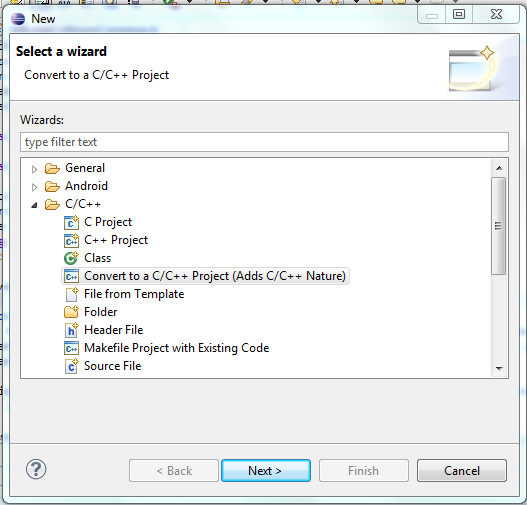
\includegraphics{./img/convert.png}
  
  7. W Properties projektu ustawić budowanie kodu w C++ przez \emph{ndk-build}.
  Najlepiej miejsce rozpakowania \emph{Android NDK} przypisać pod zmienną
  środowiskową (np. \$ \{NDKROOT\}), co ułatwi przenośność projektu.
  
  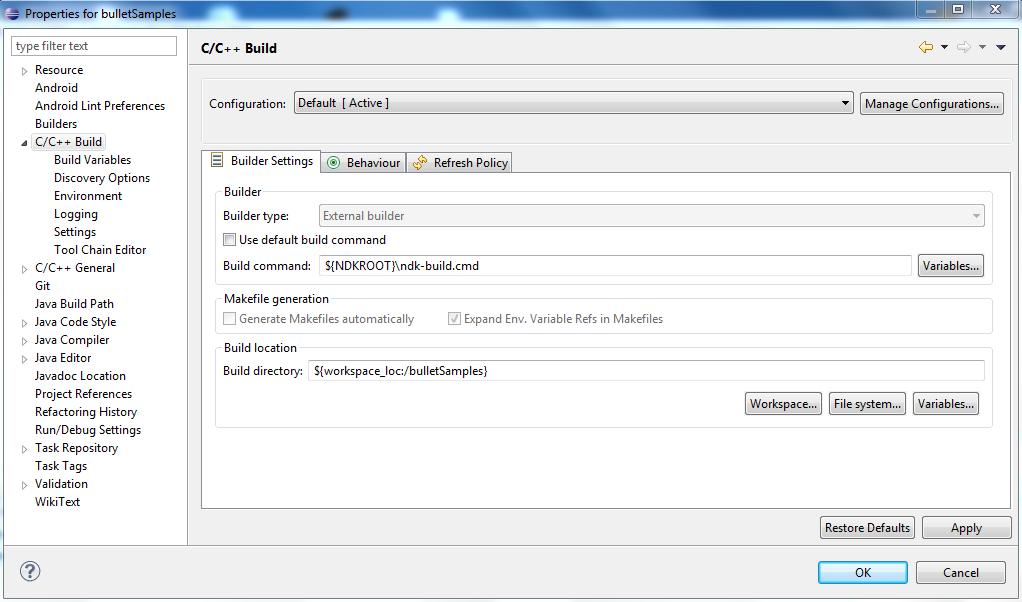
\includegraphics[width=\textwidth]{./img/properties.png}
  
  W zakładce behavior należy odznaczyć checkboxa \emph{Clean} i usunąć tekst z
  pola \emph{Build}.\\
  8. W C++ General $ \rightarrow $ Paths And Symbols dodać ścieżkę dla nagłówków.
 
  9. Ponieważ w projekcie będą wykorzystywane elementy biblioteki STL,
  konieczne jest dodanie odpowiedniej ścieżki.\\
  
  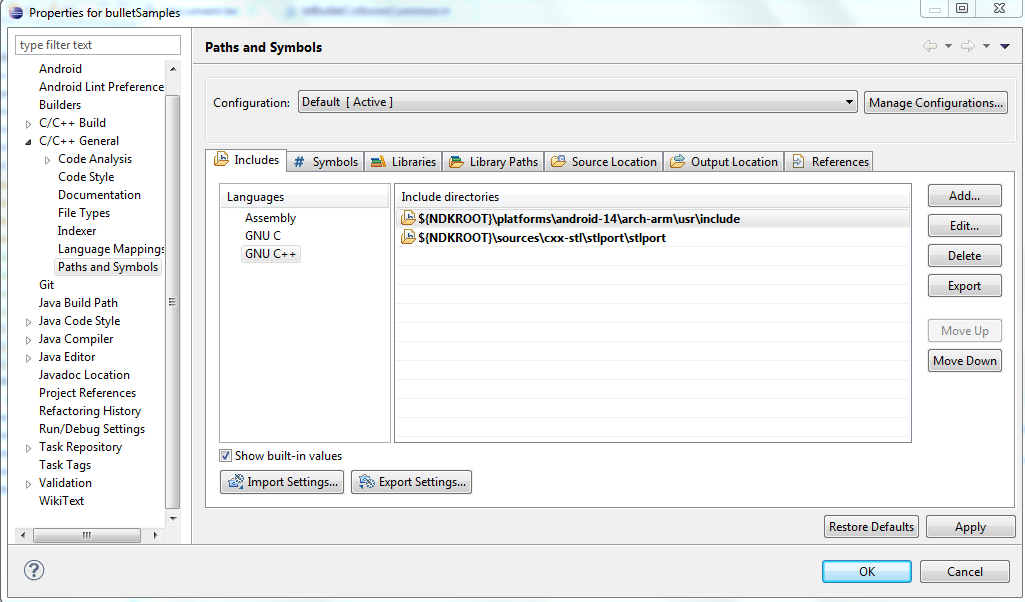
\includegraphics[width=\textwidth]{./img/ndkroot.png}
  
  Dodać również należy informację o wykorzystaniu STL w pliku
  \emph{Application.mk}(który również muisi być dodany do projektu).
  
  \lstinputlisting[language=make, caption=Zawartość pliku Application.mk,
  label=andMake]{./listings/Application.mk}
  
  Po tych czynnościach można edytować projekt ze składnią Javy jak i C++,
  korzystając z autouzupełniania i jednolitej kompilacji. Należy jednak
  pamiętać, że przy dodawaniu nowego pliku z kodem źródłowym w C++ do folderu
  \emph{jni} konieczne jest umieszczenie o nim informacji w \emph{Android.mk} .

\subsection{Wywoływanie funkcji natywnych z poziomu Javy}
Do wywoływania funkcji natywnych z poziomu języka Java Android NDK wykorzystuje
interfejs JNI. Aby dodać w kodzie C/C++ funkcję możliwą do wywałania z
wirtualnej maszyny Dalvik, w kodzie w języku Java należy użyć słowa kluczowego
\emph{native}.

\lstinputlisting[language=java, linerange={1-2, 9-9, 25-25}, caption=Użycie
słowa kluczowego native w języku Java, label=lis:javaNative]{./listings/CollisionShape.java}

Następnie w kodzie natywnym zaimplementować zarejestrowaną metodę przy pomocy
nazewnictwa
Java\_$<$nazwa\_paczki$>$\_$<$nazwa\_obiektu$>$\_$<$nazwa\_metody$>$, oraz
makra JNIEXPORT. Funkcja taka posiada dwa stałe argumenty. Pierwszym argumentem
funkcji jest wskaźnik na zmienną typu \emph{JNIEnv}, która jest interfejsem
środowiska uruchomieniowego Javy. Drugim jest zmienna typu \emph{jobject}
zawierająca referencję do obiektu wywołującego daną metodę.

\lstinputlisting[language=c++, linerange={3-4, 21-22}, caption=Implementacja
natywnej metody w kodzie c++,
label=lis:cppNative]{./listings/CollisionShape.cpp}

W kodzie nie może również zabraknąć odniesienia do pliku \emph{jni.h}.

\begin{lstlisting}[language=c++, caption=Użycie pliku nagłówkowego]
#include <jni.h>
\end{lstlisting}

\subsection{Kontener obiektów}
Ponieważ niemożliwy jest bezpośredni dostęp do obiektów po stronie natywnej,
w tym projekcie zostają zastosowane obiekty obudowujące. Po stronie Javy każdy
obiekt posiada unikalny identyfikator, który zostaje mu nadany przez
konstruktor w momencie jego tworzenia.

\lstinputlisting[language=java, linerange={5-6, 9-9, 26-31}, caption=Tworzenie
nowego obiektu obudowującego,
label=lis:javaGenId]{./listings/DynamicsWorld.java}

W kodzie natywnym wszystkie identyfikatory są przechowywane w mapie
\emph{pointer\_map} z biblioteki STL. Za jej pomocą kojarzone są identyfikatory
obudowujących obiektów Javy z obiektami biblioteki Bullet.

\lstinputlisting[language=c++, caption=Zawartość pliku btObjects.h\,
zawierającego mapę, label=lis:btObjects_h]{./listings/btObjects.h}

Funkcje \emph{put} i \emph{get} służą do umieszczania i pobierania obiektów
biblioteki Bullet z mapy.

\lstinputlisting[language=c++, caption=Zawartość pliku btObjects.cpp\,
implementującego kontener identyfikatorów,
label=lis:btObjects_h]{./listings/btObjects.cpp}

Z każdym wywołaniem metody \emph{put} zostaje zwiększony licznik
\emph{pointer\_map\_count}(ln. 10) dzięki czemu każy obiekt dodany do mapy
posiada unikalny identyfikator.\\
Następnie w implementacji metody \emph{constructor} przy
pomocy funkcji \emph{put} zostaje nadany nowy identyfikator i
przekazany (zwrócony) obiektowi obudowującemu z listingu \ref{lis:javaGenId}.

\begin{lstlisting}[language=c++, caption=Użycie mapy pointer\_map w
funkcji constructor.]
extern "C"
{
	JNIEXPORT jint Java_org_bulletSamples_physics_DynamicsWorld_constructor( JNIEnv* env, jobject self )
	{
		//inicjalizacja skladowych obiektow btDiscreteDynamicsWorld
		btDiscreteDynamicsWorld* dynamicsWorld = new
		btDiscreteDynamicsWorld(dispatcher,broadphase,solver,collisionConfiguration);
		return btObjects::put(dynamicsWorld);
	}
}
\end{lstlisting}

Aby uzyskać dostęp do przechowywanego przez mapę obiektu należy użyć metody
\emph{get}, przekazując jej otrzymaną przez parametr wartość \emph{id}. Ponieważ
mapa kojarzy identyfikatory ze wskaźnikami typu \emph{void*}, pobrana wartość
musi być przerzutowana na odpowiedni typ.

\begin{lstlisting}[language=c++, caption=Pobranie przechowywanego obiektu z
mapy] extern "C"
{
	JNIEXPORT void Java_org_bulletSamples_physics_DynamicsWorld_NCreateBox( JNIEnv* env, jobject self, jint id ...) 
	 {
	 	btDiscreteDynamicsWorld* dw = (btDiscreteDynamicsWorld*)btObjects::get(id);
	 	//wykonywanie operacji na pobranym obiekcie
	}
}
\end{lstlisting}

Całą sekwencję tworzenia i wykonywania akcji na obiektach przedstawiono na
poniższym diagramie.

\begin{center}
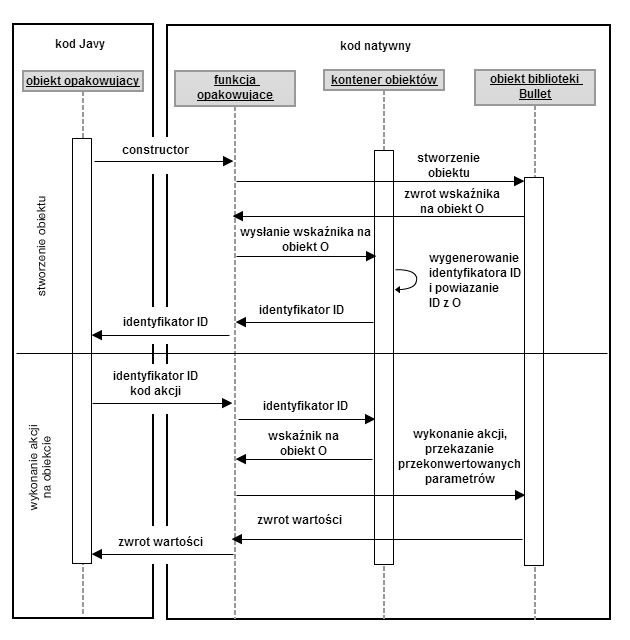
\includegraphics[width=\textwidth]{./img/sequenceDiagram.png}
\end{center}

\subsection{Struktura biblioteki obudowującej}
W celu ułatwienia składania scen testowych część klas biblioteki Bullet została
opakowana w klasach języka Java. Strukturę zawierającej je paczki przedstawia
poniższy schemat.
\begin{center}
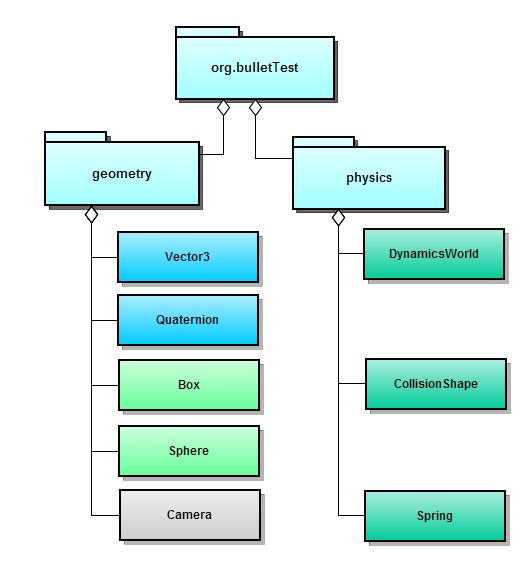
\includegraphics[scale=0.5]{./img/packageDiagram.png}
\end{center}

\subsubsection{Typy geometryczne}
Poza klasami odpowiadającymi za podstawową geometrię jak wektor (\emph{Vector3})
i kwaternion (\emph{Quaternion}), paczka \emph{org.bulletTest.geometry} zawiera
również klasy definiujące kształty - prostopadłościan (\emph{Box}) i
kulę(\emph{Sphere}). Klasy \emph{Box} i \emph{Sphere} posiadają
odpowiednie metody pozwalające na renderowanie określonych kształtów
o podanych rozmiarach.

\subsubsection{Typy fizyczne}
Dostępne metody obiektów opakowujących klasy silnika Bullet zostały
przedstawione poniżej.

\paragraph{DynamicsWorld}
Klasa przedstawia środowisko fizyczne. Dodawane są do niego symulowane bryły
sztywne i sprężyny.\\ \\
\begin{tabular}{|p{\textwidth}|}
\hline
\textbf{Klasa: DynamicsWorld}\\ \hline
\emph{Nazwa: } createShape(Mesh mesh, Vector3 position, float mass)
:CollisionShape\\
\emph{Opis: } Metoda tworzy nowy obiekt \emph{CollisionShape}(bryłę sztywną) i
dodaje go do środowiska fizycznego. Kształt i rozmiary obiektu zależą od
parametru \emph{mesh}.\\
\hline
\emph{Nazwa: } setGravity(Vector3 gravity) :void\\
\emph{Opis: } Metoda ustawia wektor przyspieszenia grawitacyjnego dla wszystkich
obiektów w środowisku.\\
\hline
\emph{Nazwa: } stepSimulation(int timeStep) :void\\
\emph{Opis: } Metoda aktualizuje symulację o podany czas w milisekundach.\\
\hline
\emph{Nazwa: } pickObject(Vector3 rayFrom, Vector3 rayTo) :void\\
\emph{Opis: } Metoda używana przez akcję ``przeciągnij i upuść\"\ opisaną w
sekcji \ref{sec:dragAndDrop}.\\
\hline
\emph{Nazwa: } dragObject(Vector3 rayFrom, Vector3 rayTo) :void\\
\emph{Opis: } Metoda używana przez akcję ``przeciągnij i upuść\"\ opisaną w
sekcji \ref{sec:dragAndDrop}.\\
\hline
\emph{Nazwa: } dropObject(Vector3 rayFrom, Vector3 rayTo) :void\\
\emph{Opis: } Metoda używana przez akcję ``przeciągnij i upuść\"\ opisaną w
sekcji \ref{sec:dragAndDrop}.\\
\hline
\emph{Nazwa: } drawDebug(GL10 gl) :void\\
\emph{Opis: } Metoda używana podczas renderowania linii pomocniczych. Opisana
jest w sekcji \ref{sec:debugDrawer}.\\
\hline
\end{tabular}

\paragraph{CollisionShape}
Klasa przedstawia symulowane obiekty brył sztywnych.\\ \\
\begin{tabular}{|p{\textwidth}|}
\hline
\textbf{Klasa: CollisionShape}\\ \hline
\emph{Nazwa: } getTransform(Vector3 position, Quaternion rotation) :void\\
\emph{Opis: } Metoda pobiera transformację obiektu: wektor pozycji oraz
kwaternion obrotu i zwraca je przez parametry.\\
\hline
\emph{Nazwa: } getTranslation() :Vector3\\
\emph{Opis: } Metoda pobiera wektor pozycji.\\
\hline
\emph{Nazwa: } getRotation() :Quaternion\\
\emph{Opis: } Metoda pobiera kwaternion obrotu.\\
\hline
\emph{Nazwa: } setTranslation(Vector3 position) :void\\
\emph{Opis: } Metoda ustawia centrum obiektu w danym punkcie.\\
\hline
\emph{Nazwa: } getRotation(Quaternion rotation) :void\\
\emph{Opis: } Metoda ustawia obrót obiektu względem podanego kwaternionu.\\
\hline
\emph{Nazwa: } applyCentralForce(Vector3 force): void\\
\emph{Opis: } Metoda działa na centrum obiektu siłą o wartości podanej w
parametrze.\\
\hline
\emph{Nazwa: } applyTorque(Vector3 torque): void\\
\emph{Opis: } Metoda działa na obiekt z momentem siły o wartości podanej w
parametrze.\\
\hline
\emph{Nazwa: } render(GL10 gl): void\\
\emph{Opis: } Metoda renderuje bryłę sztywną w oparciu o podany podczas
tworzenia obiektu kształt.\\
\hline
\emph{Nazwa: } setRestitution(float restitution): void\\
\emph{Opis: } Metoda ustawia wartość współczynnika sprężystości bryły.\\
\hline
\emph{Nazwa: } setFriction(float friction): void\\
\emph{Opis: } Metoda ustawia wartość współczynnika tarcia bryły.\\
\hline
\emph{Nazwa: } setLinearVelocity(Vector3 velocity): void\\
\emph{Opis: } Metoda ustawia wartość liniowej prędkości bryły.\\
\hline
\emph{Nazwa: } setAngularVelocity(Vector3 velocity): void\\
\emph{Opis: } Metoda ustawia wartość prędkości kątowej bryły.\\
\hline
\emph{Nazwa: } getLinearVelocity(): Vector3\\
\emph{Opis: } Metoda pobiera wartość liniowej prędkości bryły.\\
\hline
\emph{Nazwa: } getAngularVelocity(): Vector3\\
\emph{Opis: } Metoda pobiera wartość prędkości kątowej bryły.\\
\hline
\end{tabular}

\paragraph{Spring}\label{sec:spring}
Klasa przedstawia symulowane obiekty ciał sprężystych.\\
W parametrach funkcji można znaleźć typ enumeracyjny \emph{DoF} -
stopnie swobody (\emph{degrees of freedom}). Określają one do jakiego stopnia
swobody odnosi się dane wywołanie metody. Dostępne wartości to:\\
\begin{tabular}{|p{\textwidth}|}
\hline
\textbf{Enum: Dof}\\ \hline
translateX\\
translateY\\
translateZ\\
rotateX\\
rotateY\\
rotateZ\\
\hline
\end{tabular}
\\ \\
Do zaobrazowania znaczenia poszczególnych parametrów funkcji klasy Spring
zostanie wykorzystana poniższa scena:\\

\lstinputlisting[language=java, caption=Scena demonstrująca użycie klasy Spring,
label=lis:spring_demo]{./listings/spring_demo.java}

\begin{figure}
\centering
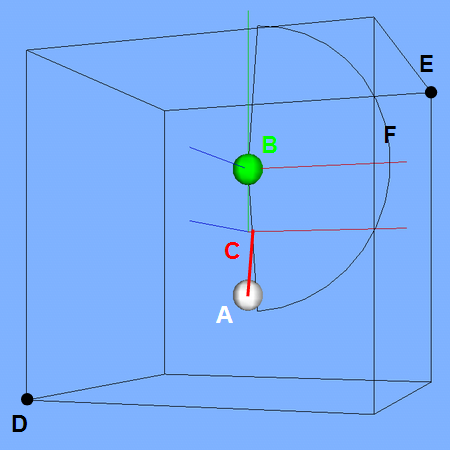
\includegraphics[scale = 0.6]{./img/Spring-render.png}
\caption{Render sceny z listingu \ref{lis:spring_demo}.}
\label{fig:spring_demo}
\end{figure}

Opisy metod w poniższej tabeli odnoszą się do oznaczeń na rysunku
\ref{fig:spring_demo}. Wszystkie metody działąjące na stopień swobody sprężyny
odnoszą się do ciała oznaczonego przez \textbf{B}.\\
\begin{tabular}{|p{\textwidth}|}
\hline
\textbf{Klasa: Spring}\\
\hline
\emph{Nazwa: } konstruktor(CollisionShape shapeA, CollsionShape shapeB, Vector3
frameInA, Vector3 frameInB)\\
\emph{Opis: } Tworzona sprężyna łączy ze sobą dwa obiekty \emph{shapeA} -
oznaczone na rysunku przez ciało \textbf{A} i \emph{shapeB} - oznaczone przez
ciało \textbf{B}. Parametr \emph{frameInA} określa wektor przesunięcia ramki
ograniczającej swobodę zawieszonego ciała \textbf{B} oznaczony na rysunku przez
wektor \textbf{C}. Parametr \emph{frameInB} odpowiada za wektor przesunięcia
ciała \textbf{B} względem ograniczenia osi obrotu(oznaczonego przez łuk
\textbf{F}).\\
\hline
\emph{Nazwa: } enable(Dof index, boolean enable) :void\\
\emph{Opis: } Metoda odblokowuje dany stopień swobody.\\
\hline
\emph{Nazwa: } setDamping(Dof index, float damping): void\\
\emph{Opis: } Metoda ustawia wartość współczynnika tłumienia dla danego
stopnia swobody.\\
\hline
\emph{Nazwa: } setStiffness(Dof index, float stiffness) :void\\
\emph{Opis: } Metoda ustawia wartość współczynnika sztywności dla danego
stopnia swobody.\\
\hline
\emph{Nazwa: } setupDof(Dof index, float stiffness, float damping) :void\\
\emph{Opis: } Metoda pozwalająca na równoczesne ustawienie współczynnika
sztywności i tłumienia dla danego stopnia swobody.\\
\hline
\emph{Nazwa: } setLinerUpperLimit(Vector3 vec) :void i
setLinerLowerLimit(Vector3 vec) :void\\
\emph{Opis: } Wektory \emph{vec} określają kolejno dolne i górne wartości ramki
ograniczającej swobodę ciała \textbf{B}. Środek ramki znajduje się w pozycji
ciała \textbf{A} i jest przesunięty o wektor \emph{frameInA} podany w
konstruktorze. Na rysunku pozycję ograniczenia ramki oznaczono przez punkty
\textbf{D} i \textbf{E}.\\
\hline
\emph{Nazwa: } setAngularUpperLimit(Vector3 vec) :void i
setAngularLowerLimit(Vector3 vec) :void\\
\emph{Opis: } Metody określają odpowiednio górny i dolny limit rotacji ciała
\textbf{B}. Na rysunku ograniczenie jest oznaczone przez łuk \textbf{F}. Ciało
\textbf{B} może być przesunięte względem środka ograniczenia obrotu o wektor
\emph{frameInB} podany w konstruktorze klasy Spring.\\
\hline
\end{tabular}

\subsection{Przekazywanie argumentów i zwracanych wartości}
Podczas wymiany argumentów przez funkcje między wirtualną maszyną Javy a kodem
natywnym podstawowe typy danych (jak \emph{int} czy \emph{float}) zostają
przekonwertowane przez interfejs JNI na im odpowiadające dla danego środowiska.
Natomiast gdy przekazywane są typy złożone (jak \emph{Vector3} i
\emph{Quaternion} w bibliotece \emph{org.bulletTest.geometry}), wartości
otrzymywane w parametrach to referencje na dany obiekt. W takich przypadkach
konwersja musi być wykonana przez kod aplikacji poprzez pobranie i odpowiednie
przypisanie pól z typami podstawowymi. Poniższy listing przedstawia metodę
zamieniającą obiekt Javy \emph{Vector3} na natywny obiekt klasy \emph{btVector3}
z biblioteki Bullet.

\lstinputlisting[language=c++, caption=Konwersja klasy Vector3 z obiektu Javy
do obiektu natywnego., label=lis:jnVector3Conv,
linerange={39-50}]{./listings/common.cpp}

Parametr \emph{env} to referencja do środowiska uruchomieniowego Javy,
\emph{obj} jest referencją na obiekt Javy \emph{Vector3}, a \emph{vec} to
zwrócony przekonwertowany obiekt \emph{btVector3}. Przy pomocy metody
\emph{GetObjectlClass} (ln. 3) zostaje pobrana zmienna reprezentująca klasę
obiektu \emph{obj}, która zostaje wykorzystana przez metody
\emph{GetFieldId} (ln. 4-6) do pobrania reprezentacji pól obiektu. Następnie za
ich pomocą wyciągnięte zostają same wartości pól - współrzędnych \emph{x},
\emph{y} i \emph{z} wektora (ln. 8-10), które zostają wykorzystane do stworzenia
nowego obiektu natywnego klasy \emph{btVector3}. Analogicznie realizowana jest
konwersja obiektów natywnych na obiekty Javy.

\subsection{Zwalnianie pamięci}
Gdy dany opakowujący klasę biblioteki Bullet obiekt przestaje być potrzebny
należy zwolnić zajmowaną przez niego pamięć. Niestety wbudowany w maszynę
wirtualną Dalvik odśmiecacz pamięci (\emph{garbage collector}) nie może usunąć
obiektu natywnego. Do tego celu wymagane jest zaimplementowanie destruktora dla
klasy opakowującej. Pierwszym krokiem jest przeciążenie metody \emph{finalize}
wywoływanej podczas usuwania obiektu Javy przez odśmiecacz.

\begin{lstlisting}[language=Java, caption=Przeciążenie metody \emph{finalize}
na przykładzie klasy \emph{DynamicsWorld}] public class DynamicsWorld
{
	...
	native private void destructor(int id);
	...
	protected void finalize() throws Throwable
	{
		destructor(id);
		super.finalize();
	}
	...
}
\end{lstlisting}

Następnie należy zaimplementować funkcję destruktora w kodzie natywnym.

\begin{lstlisting}[language=c++, caption=Implementacja funkcji
\emph{destructor} na przykładzie klasy \emph{DynamicsWorld}]
JNIEXPORT void Java_org_bulletSamples_physics_DynamicsWorld_destructor( JNIEnv* env, jobject self, jint id )
{
	delete (btDiscreteDynamicsWorld*)btObjects::get(id);
	btObjects::remove(id);
}
\end{lstlisting}

W linijce 3 pobierany jest wskaźnik na obiekt typu
\emph{btDiscreteDynamicsWorld} a następnie wskazywany przez niego obiekt jest
usuwany za pomocą polecenia \emph{delete}. W linijce 4 usuwany jest
identyfikator wraz z wskaźnikiem na nieistniejący już obiekt z mapy
\emph{btObjects}.

\subsection{Sceny}
W celu ułatwienia dodawania kolejnych testów silnika powstał mechanizm scen,
które można wymieniać przed kompilacją aplikacji. Każda scena zawiera właściwe
dla siebie obiekty fizyczne i związane z nimi instrukcje. Klasa \emph{BaseScene}
jest klasą bazową dla wszystkich scen w projekcie.

\begin{figure}
\centering
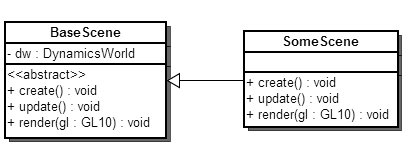
\includegraphics[scale=0.6]{./img/SceneClassDiagram.png}
\caption{Diagram reprezentujący klasę SomeScene.}
\label{fig:sceneClassDiagram}
\end{figure}

Każda scena posiada własny egzemplarz klasy \emph{DynamicsWorld} nadawany jej
przez konstruktor. Przeciążając metody \emph{create}, \emph{update} i
\emph{render} można na scenie wykonać każdą akcję.

\newpage
\section{Implementacja i zastosowanie dodatkowych możliwośći silnika Bullet}
W tej części pracy zostanie opisany przebieg implementacji dodatkowych funkcji
wykorzystujących możliwości oferowane przez platformy mobilne i silnik Bullet.
%\emph{TODO:
%w jaki sposób zostały zaimplementowane pozostałe przydatne mechanizmy silnika i
%jak zostały wykorzystane możliwości smartphone'a do uatrakcyjnienia
% aplikacji:)}

\subsection{Akcelerometr}
%http://developer.android.com/guide/topics/sensors/sensors_overview.html
Większość smartfonów i tabletów obecnej generacji wyposażona jest w
akcelerometr. Urządzenie to może być wykorzystane na przykład do sterowania
kierunkiem przyspieszenia grawitacyjnego lub kątem ustawienia kamery w
symulacji.

Na początku należy stworzyć statyczną klasę przechowującą pobrany wektor
przyspieszenia z akcelerometru.

\begin{lstlisting}[language=java, caption=Klasa Accelerometer przechowująca
dane pobrane z akcelerometru.]
package org.bulletSamples;
 
import org.bulletSamples.geometry.Vector3;
 
public class Accelerometer
{
	public static Vector3 gravity = new Vector3();
}
\end{lstlisting}

W systemie Android dostęp do akcelerometru uzyskuje się poprzez statyczną klasę
\emph{SensorManager}.

\begin{lstlisting}[language=java, caption=Pobranie wektora przyspieszenia z
akcelerometru.] public class BulletTestActivity extends Activity implements SensorEventListener {

	public void onCreate(Bundle savedInstanceState) {
		...
		mSensorManager = (SensorManager)getSystemService(SENSOR_SERVICE);
		mAccelerometer = mSensorManager.getDefaultSensor(Sensor.TYPE_GRAVITY);
    }
    
	...
    
    public void onSensorChanged(SensorEvent event) {
		Accelerometer.gravity.x = event.values[0];
		Accelerometer.gravity.y = event.values[1];
		Accelerometer.gravity.z = event.values[2];
	}
}
\end{lstlisting}

Główne \emph{activity} aplikacji musi implementować interfejs
\emph{SensorEventListener}. 

Każda oś wektora \emph{Accelerometer}.\emph{gravity} odpowiada osi nachylania
urządrzenia na którym uruchomiona jest aplikacja. Rozkład tych osi
zaprezentowano na rysunku \ref{fig:axis_device}.

\begin{figure}
\centering
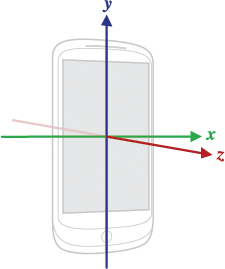
\includegraphics[scale = 0.6]{./img/axis_device.png}
\caption{Rozłożenie osi wektora przyspieszenia dla akcelerometru w urządzeniu
z systemem Android.}
\label{fig:axis_device}
\end{figure}

Tak pobrane wartości wektora akcelerometru można wykorzystać do sterowania
przyspieszeniem grawitacji aplikacji. W tym celu we fragmencie odpowiedzialnym
za rendering sceny można umieścić odpowiedni kod.

\begin{lstlisting}[language=java, caption=Sterowanie wektorem przyspieszenia
ziemskiego przy pomocy akcelerometru]import org.bulletSamples.Accelerometer;
import org.bulletSamples.geometry.*;
import org.bulletSamples.physics.*;

public class SomeScene extends BaseScene {
	...
	
	public void render(GL10 gl)
	{
		dw.setGravity(Accelerometer.gravity);
		//kod odpowiedzialny za rendering obiektow na scenie
	}
}
\end{lstlisting}

Akcelerometr można również zastosować do sterowania innymi parametrami jak na
przykład kątem nachylenia kamery.

\begin{lstlisting}[language=java, caption=Sterowanie kątem nachylenia kamery
przy pomocy akcelerometru, label=lis:accCamera]import org.bulletSamples.Accelerometer;
import org.bulletSamples.geometry.*;
import org.bulletSamples.physics.*;

public class SomeScene extends BaseScene {
	...
	
	public void render(GL10 gl)
	{
		Camera.active.position = Accelerometer.gravity.normalize().multiply(60);
		//kod odpowiedzialny za rendering obiektow na scenie
	}
}
\end{lstlisting}

Na listingu \ref{lis:accCamera} w linijce 21 zastosowano wektor pobrany z
akcelerometru i pomnożony przez skalar 60 jako wektor pozycji dla kamery na
scenie.

\subsection{Przeciągnij i upuść}\label{sec:dragAndDrop}
Inną możliwością wprowadzenia interakcji w aplikacji jest wykorzystanie ekranu
dotykowego dostępnego w większości produkowanych dziś urządzeń mobilnych.
Możliwe jest dzięki temu wprowadzenie funkcji ``przeciągnij i upuść''
(\emph{drag and drop}), dzięki czemu możliwe będzie złapanie dowolnego obiektu
fizycznego i przeniesienie go w inne miejsce palcem po ekranie.

Pierwszym krokiem jest zamiana współrzędnych ekranu (miejsca w którym ekran
został dotkniętuy palcem) na współrzędne świata silnika fizycznego. Proces ten
został przedstawiony na rysunku \ref{fig:raycast}.

\begin{figure}
\centering
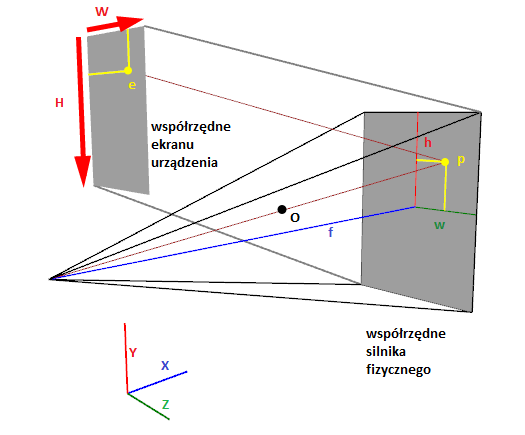
\includegraphics[scale = 0.8]{./img/Rzutowanie.png}
\caption{Rzutowanie współrzędnych ekranu na współrzędne świata silnika}
\label{fig:raycast}
\end{figure}

Następnie zostaje poprowadzona linia (\emph{raycast}) od ``oka'' do
przerzutowanego punktu we spółrzędnych silnika (na rysunku
oznaczonego przez \textbf{p}). ``Podniesiony'' zostaje obiekt przecinający się z
poprowadzoną linią (obiekt \textbf{O}).

Zamianę współrzędnych należy zacząć od zmiany układu współrzędnych. W
urządzeniach z systemem Android przebieg osi oznaczono na rysunku
\ref{fig:raycast} czerwonymi strzałkami. W silniku fizycznym osie oznaczono
żółtą i zieloną linią. Odpowiednie przekształcenie dokonywane jest przez macierz
ze wzoru \ref{eq:srodek}.

\begin{equation}p_{t} = 
p_{e}
\begin{bmatrix}1&0&0&0\\0&-1&0&0\\0&0&1&0\\-w_{e}&h_{e}&0&1\end{bmatrix}
\label{eq:srodek}
\end{equation}

Gdzie:\\
$ p_{t} = \begin{bmatrix}x_{t}&y_{t}&0&1\end{bmatrix} $ to przetransportowany
wektor punktu\\
$ p_{e} = \begin{bmatrix}x_{e}&y_{e}&0&1\end{bmatrix} $ to wektor pobranych
współrzędnych ekranowych\\
$ w_{e} $ i $ h_{e} $ to kolejno połowa szerokości i wysokości ekranu urządzenia
w pikselach
\\ \\
Następnie należy dokonać przeskalowania pobranych współrzędnych aby były one
zgodne ze skalą płaszczyzny rzutowania (płaszczyzny na której znajduje się
punkt \textbf{p} z rysunku \ref{fig:raycast}). Przekształcenie to jest
dokonywane przez następującą zależność:

\begin{equation}
\frac{y_{t}}{h_{e}}=\frac{y_{p}}{h_{p}}
\label{eq:przeksz}
\end{equation}

Gdzie:\\
$ y_{p} $ to przetransformowana współrzędna na płaszczyźnie rzutowania\\
$ h_{p} $ to wysokość płaszczyzny rzutowania oznaczona na rysunku
\ref{fig:raycast} przez \textbf{h}\\
Wysokość płaszczyzny rzutowania jest zależna od \emph{FoV} (\emph{field of
view}) - kąta pola widzenia i może być obliczona w następujący sposób:

\begin{equation}
h_{p} = f \tg \alpha
\label{eq:alpha}
\end{equation}
\emph{f} to odległość ``oka'' od płaszczyzny rzutowania (na rysunku oznaczona
niebieską linią)\\
$ \alpha $ to połowa kąta \emph{FoV}. Ponieważ obliczaną wysokością jest połowa
wysokości płaszczyzny rzutowania, w tym miejscu zostaje zastosowana połowa
kąta.\\
\\
Korzystając ze wzorów \ref{eq:przeksz} i \ref{eq:alpha} otrzymuje się zależność:

\begin{equation}
y_{p} = \frac{fy_{t} \tg \alpha}{h_{e}}
\end{equation}

W celu zachowania proporcji generowanego obrazu współrzędna o mniejszej
maksymalnej wartości przekształcona zostaje jak współrzędna o większej
maksymalnej wartości. Na potrzeby tych obliczeń przyjęte zostaje, że $ w_{e} <
h_{e} $, czyli wartość \emph{x} zostaje obliczana jak wartość \emph{y}.
Omawiane przeskalowanie zostaje wykonane przez poniższą macierz:

\begin{equation}
\begin{bmatrix}\frac{f \tg \alpha}{h_{e}}&0&0&0\\0&\frac{f \tg \alpha}{h_{e}}&0&0\\0&0&1&0\\0&0&p&1\end{bmatrix}
\label{eq:scale}
\end{equation}

Mnożąc macierze \ref{eq:srodek} i \ref{eq:scale} otrzymana zostaje macierz
rzutowania punktu z współrzędnych ekranowych na współrzędne silnika fizycznego:

\begin{equation}
S = 
\begin{bmatrix}1&0&0&0\\0&-1&0&0\\0&0&1&0\\-w_{e}&h_{e}&0&1\end{bmatrix}
\begin{bmatrix}\frac{f \tg \alpha}{h_{e}}&0&0&0\\0&\frac{f \tg
\alpha}{h_{e}}&0&0\\0&0&1&0\\0&0&p&1\end{bmatrix} =
\begin{bmatrix}\frac{f \tg \alpha}{h_{e}}&0&0&0\\0&-\frac{f \tg
\alpha}{h_{e}}&0&0\\0&0&1&0\\-\frac{w_{e}f \tg \alpha}{h_{e}}&f \tg \alpha&p&1\end{bmatrix}
\end{equation}

Korzystając z powyższej macierzy można otrzymać współrzędne punktu do którego
zostaje poprowadzona linia ($ p_{p} $) wybierająca chwytany obiekt.

\begin{equation}
p_{p} = p_{e} S W
\label{eq:transform}
\end{equation}
Gdzie:\\
$ p_{p} $ i $ p_{e} $ to wektory postaci:\\
$ p_{p} = \begin{bmatrix}x_{p}&y_{p}&z_{e}&1\end{bmatrix} $ \\
$ p_{e} = \begin{bmatrix}x_{e}&y_{e}&0&1\end{bmatrix} $ \\
\emph{W} to macierz świata wyświetlanej sceny (iloczyn odwrotnej macierzy
translacji kamery i odwrotnego obrotu kamery).\\
\\ \\
Aby funkcja ``przeciągnij i upuść'' działała, konieczne jest przechwycenie przez
aplikację zdarzenia dotknięcia ekranu dotykowego urządzenia, co prezentuje
listing \ref{lis:onTouch}.

\begin{lstlisting}[language=java, caption=Przechwycenie zdarzenia
dotknięcia ekranu.,label=lis:onTouch]public void onTouch(MotionEvent e)
{
	int x = (int)e.getX();
	int y = (int)e.getY();
	int eventaction = e.getAction();
	Vector3 rayFrom;
	if(Camera.active != null) rayFrom = Camera.active.getPosition();
	else rayFrom = Vector3.zero();
    switch (eventaction ) { 
    	case MotionEvent.ACTION_DOWN:
    		dw.pickObject(rayFrom, getRayTo(x, y));
    		break;
    	case MotionEvent.ACTION_MOVE:
    		dw.dragObject(rayFrom, getRayTo(x, y));
    		break;
    	case MotionEvent.ACTION_UP:
    		dw.dropObject(rayFrom, getRayTo(x, y));
    		break;
    }
}
\end{lstlisting}

Obiket \emph{dw} jest obiektem klasy \emph{DynamicsWorld}. Funkcja
\emph{getRayTo} wykonuje operację ze wzoru \ref{eq:transform}.\\

Implementacja metody \emph{pickObject}, wywoływanej po naciśnięciu obiektu na
ekranie, wygląda następująco:

\begin{lstlisting}[language=c++, caption=Implementacja
metody pickObject,label=lis:pickObject]
JNIEXPORT void Java_org_bulletSamples_physics_DynamicsWorld_NpickObject( JNIEnv* env, jobject self, jint id, jobject jRayFrom, jobject jRayTo )
{
	btDiscreteDynamicsWorld* dw = (btDiscreteDynamicsWorld*)btObjects::get(id);
	btVector3 rayFrom, rayTo;
	jobjectToBtVector3(env, jRayFrom, rayFrom);
	jobjectToBtVector3(env, jRayTo, rayTo);
	btCollisionWorld::ClosestRayResultCallback rayCallback(rayFrom,rayTo);
	dw->rayTest(rayFrom,rayTo,rayCallback);
	if (rayCallback.hasHit())
	{
		btRigidBody* body = btRigidBody::upcast(rayCallback.m_collisionObject);
		if (body)
		{
			if (!(body->isStaticObject() || body->isKinematicObject()))
			{
				pickedBody = body;
				pickedBody->setActivationState(DISABLE_DEACTIVATION);
				btVector3 pickPos = rayCallback.m_hitPointWorld;
				btVector3 localPivot = body->getCenterOfMassTransform().inverse() * pickPos;
				btTransform tr;
				tr.setIdentity();
				tr.setOrigin(localPivot);
				btGeneric6DofConstraint* dof6 = new btGeneric6DofConstraint(*body, tr,false);
				dof6->setLinearLowerLimit(btVector3(0,0,0));
				dof6->setLinearUpperLimit(btVector3(0,0,0));
				dof6->setAngularLowerLimit(btVector3(0,0,0));
				dof6->setAngularUpperLimit(btVector3(0,0,0));
				dw->addConstraint(dof6);
				pickConstraint = dof6;
				oldPickingPos = rayTo;
				hitPos = pickPos;
				oldPickingDist  = (pickPos-rayFrom).length();
			}
		}
	}
}
\end{lstlisting}

Na początku zostaje wykonany \emph{raytest} - sprawdzenie czy obiekt nie
znajduje się na linii od \emph{rayFrom} do \emph{rayTo} (ln. 8-16). Następnie
wygenerowane zostaje ciało sprężyste (ln.23-27) łączące napotkane ciało z
punktem aktualnego zderzenia. Wiekszość wartości zostaje zapisana w wartościach
globalnych, ponieważ są potrzebne do działania pozostałych funkcji (ln.
16,29-32).

Metoda \emph{dragObject} jest wywoływana podczas przesuwania obiektu po
ekranie.

\begin{lstlisting}[language=c++, caption=Implementacja
metody dragObject,label=lis:dragObject]
JNIEXPORT void Java_org_bulletSamples_physics_DynamicsWorld_NdragObject( JNIEnv* env, jobject self, jint id, jobject jRayFrom, jobject jRayTo )
{
	if(pickConstraint == 0) return;
	btDiscreteDynamicsWorld* dw = (btDiscreteDynamicsWorld*)btObjects::get(id);
	btVector3 rayFrom, rayTo;
	jobjectToBtVector3(env, jRayFrom, rayFrom);
	jobjectToBtVector3(env, jRayTo, rayTo);
	btGeneric6DofConstraint* pickCon = static_cast<btGeneric6DofConstraint*>(pickConstraint);
	btVector3 newRayTo = rayTo;
	btVector3 oldPivotInB = pickCon->getFrameOffsetA().getOrigin();
	btVector3 newPivotB;
	btVector3 dir = newRayTo-rayFrom;
	dir.normalize();
	dir *= oldPickingDist;
	newPivotB = rayFrom + dir;
	pickCon->getFrameOffsetA().setOrigin(newPivotB);
}
\end{lstlisting}

Przechowywana sprężyna w zmiennej \emph{pickConstraint} otrzymuje nowe
współrzędne ramek w których trzymany jest obiekt. Sa one obliczone na podstawie
wczęniej przechowanyvh wartości.

Ostatnia metoda \emph{dropObject} jest wywoływana po oderwaniu palca od
powierzchni ekranu.

\begin{lstlisting}[language=c++, caption=Implementacja
metody dropObject,label=lis:dropObject]
JNIEXPORT void Java_org_bulletSamples_physics_DynamicsWorld_NdropObject( JNIEnv* env, jobject self, jint id, jobject jRayFrom, jobject jRayTo )
{
	btDiscreteDynamicsWorld* dw = (btDiscreteDynamicsWorld*)btObjects::get(id);
	dw->removeConstraint(pickConstraint);
	delete pickConstraint;
	pickConstraint = 0;
	pickedBody->forceActivationState(ACTIVE_TAG);
	pickedBody->setDeactivationTime( 0.f );
	pickedBody = 0;
}
\end{lstlisting}

Po zaimplementowaniu powyższych funkcji w aplikacji możliwe jest przenoszenie
widocznych na ekranie obiektów.

\subsection{Linie pomocnicze}\label{sec:debugDrawer}
W celu ułatwienia projektowania symulacji mozna wykorzystać
wbudowaną w silniku bullet możliwość rysowania linii pomocniczych (\emph{debug
draw}). Linie te zaznaczają miedzy innymi limity obrotów i wielkość ramki ciała
zawieszonego na sprężynie. Rysowane linie pomocnicze można zauważyć na rysunku
\ref{fig:spring_demo}.\\
Aby możliwe było korzystanie z możliwości rysowania linii pomocniczych, należy
zaimplementować interfejs silnika bullet \emph{btIDebugDraw}. Interfejs ten
posiada metody odpowiadające za rysowanie prostych kształtów (np. \emph{drawLine}).
Implementacja poszczególych metod pozwala na niezależne od silnika renderującego
wyświetlanie pomocniczych kształtów.

W tym przykładzie zostanie zaimplementowana metoda \emph{drawLine}.
Implementacja interfejsu w kodzie natywnym wygląda następująco:

\begin{lstlisting}[language=c++, caption=Deklaracja klasy
DebugDrawer,label=lis:debugDrawer_cpp]
class DebugDrawer : public btIDebugDraw
{
public:
	DebugDrawer();
	virtual void drawLine(const btVector3& from,const btVector3& to,const btVector3& color); 
	...
};

void DebugDrawer::drawLine(const btVector3& from,const btVector3& to,const btVector3& fromColor, const btVector3& toColor)
{
	jclass claz = globalEnv->FindClass("org/bulletSamples/physics/DebugDrawer");
	jmethodID mid = globalEnv->GetStaticMethodID(claz, "drawLine", "(Lorg/bulletSamples/geometry/Vector3;Lorg/bulletSamples/geometry/Vector3;Lorg/bulletSamples/geometry/Vector3;Lorg/bulletSamples/geometry/Vector3;)V");
	globalEnv->CallStaticVoidMethod(claz, mid, jVector3(globalEnv, from), jVector3(globalEnv, to), jVector3(globalEnv, fromColor), jVector3(globalEnv, toColor));
}
\end{lstlisting}

Metoda \emph{DebugDrawer::drawLine} odnosi sie do statycznej metody
\emph{drawLine} klasy \emph{DebugDrawer} zaimplementowanej w Javie. W linijce
11 pobrany zostaje identyfikator metody, który zostaje wykorzystany do jej
wywołania w linijce 12 , przekazując jej swoje parametry wywołania. Zmienna
\emph{globalEnv}, jest przechowywaną globalnie zmienną zawierającą wskażnik na
środowisko uruchomieniowe Javy. Jest ona odświeżana przy każdej rysowanej
ramce. Ponieważ metoda \emph{drawLine} nie jest bezpośrednio wywoływana przez
metodę w środowisku Javy, a przez obiekt klasy \emph{DynamicsWorld}, nie ma ona
dostępu do obiektu \emph{env} przez parametr. W kodzie natywnym pobranie
zmiennej \emph{globalEnv} wygląda nstępująco:

\begin{lstlisting}[language=c++, caption=Deklaracja
funkcji renewEnv w kodzie natywnym,label=lis:renewEnvNat]
JNIEnv* globalEnv = 0;

extern "C"
{
	JNIEXPORT void Java_org_bulletSamples_physics_DebugDrawer_renewEnv(JNIEnv* env, jclass claz)
	{
		globalEnv = env;
	}
}
\end{lstlisting}

Natomiast w kodzie Javy:

\begin{lstlisting}[language=c++, caption=Deklaracja
i wykorzystanie metody renewEnv w kodzie Javy,label=lis:renewEnvJav]
public class DebugDrawer {
	public static native void renewEnv();
	...
}

public class DynamicsWorld {
	...
	public void drawDebug(GL10 gl)
	{
		DebugDrawer.gl = gl;
		gl.glLoadIdentity();
		Camera.applyTransform(gl);
		DebugDrawer.renewEnv();
		NdrawDebug();
	}
}
\end{lstlisting}

Pobieranie globalnego obiektu \emph{env} odbywa się przy każdym odrysowywaniu
linii pomocniczych (w metodzie \emph{drawDebug} ln. 13).\\
Posiadając klasę implementującą metodę \emph{drawLine} możliwe jest przypisanie
obiektu tej klasy do obiektu klasy \emph{DebugDrawer}. Przypisanie to następuje
w konstruktorze klasy \emph{DebugDrawer}.

\begin{lstlisting}[language=c++, caption=Przypisanie
obiektu DebugDrawer obiektowi DynamicsWorld,label=lis:DynamicsWorldConstructor]
JNIEXPORT jint Java_org_bulletSamples_physics_DynamicsWorld_constructor( JNIEnv* env, jobject self )
{
	...
    DebugDrawer* dd = new DebugDrawer;
    dd->setDebugMode(btIDebugDraw::DBG_DrawConstraints+btIDebugDraw::DBG_DrawConstraintLimits);
    dynamicsWorld->setDebugDrawer(dd);

	return btObjects::put(dynamicsWorld);
}
\end{lstlisting}

Po wprowadzeniu powyższych funkcji i zastosowaniu metody
\emph{DebugDrawer.drawDebug} w funkcji renderującej, wyświetlane są linie
pomocnicze. Jednak po kilku klatkach aplikacja przestaje działać. W rejestrze
błędów można zobaczyć:

\begin{figure}
\centering
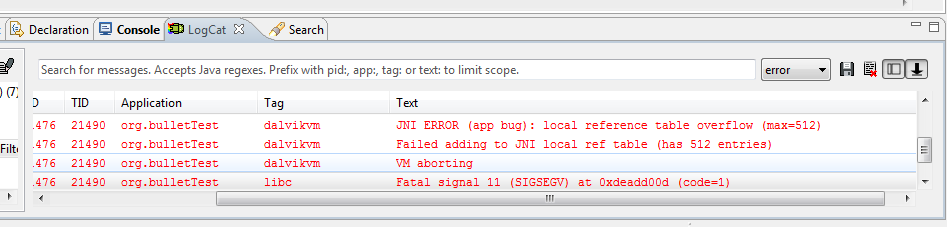
\includegraphics[scale = 0.6]{./img/logCat.PNG}
\caption{Błędy widoczne po próbie zastosowania klasy DebugDrawer.}
\label{fig:logCat}
\end{figure}

Widoczny błąd spowodowany jest przepełnieniem lokalnego bufora JNI. Podczas
przekazywania parametrów przez funkcję \emph{drawLine} z listingu
\ref{lis:debugDrawer_cpp} obiekty przekazywane przez parametry przechowywane są
w lokalnym buforze JNI, który ma ograniczoną pojemność. Problem ten można ominąć
przez użycie tymczasowych, statycznych zmiennych przechowujących przekazywane
parametry metodzie \emph{drawLine} po stronie Javy.

\begin{lstlisting}[language=Java,
caption=Tymczasowe zmienne przechowujące
parametry wywołania metody drawLine,label=lis:dummyVals] public
class DebugDrawer
{
	...
	public static Vector3 dummy1 = Vector3.zero(), dummy2 = Vector3.zero(), dummy3 = Vector3.zero(), dummy4 = Vector3.zero(); 
	...
}
\end{lstlisting}

Kod funkcji \emph{DebugDrawer::drawLine} z listingu \ref{lis:debugDrawer_cpp}
powinien wtedy wyglądać:

\begin{lstlisting}[language=C++,
caption=Implementacja metody drawLine
korzystającej z tymczasowych zmiennych,label=lis:drawLineDummyVals]
void DebugDrawer::drawLine(const btVector3& from,const btVector3& to,const btVector3& color)
{
	jclass claz = globalEnv->FindClass("org/bulletSamples/physics/DebugDrawer");
	jmethodID mid = globalEnv->GetStaticMethodID(claz, "drawLine", "()V");
	setNamedVector3(globalEnv, claz, "dummy1", from); setNamedVector3(globalEnv, claz, "dummy2", to); 
	setNamedVector3(globalEnv, claz, "dummy3", color);
	setNamedVector3(globalEnv, claz, "dummy4", color);
	globalEnv->CallStaticVoidMethod(claz, mid);
}
\end{lstlisting}

Po tym zabiegu możliwe jest bezbłędne renderowanie linii pomocniczych na scenie.

%\subsection{Wykrywanie kolizji}
%\emph{TODO: o możliwości logowania kolizkji wybranych obiektów}

\newpage
\section{Wykorzystanie silnika Bullet w doświadczeniach fizycznych}
Do tej pory rozważane była jedynie kwestia samego działania silnika na
platformie Android. Jakie jednak niesie on możliwości pod kątem symulacji
fizycznych? Jako wysokowydajnościowy silnik Bullet nie ma wysokiej precyzji
pomiarów, ale możliwe jest sprawdzenie w jakich warunkach wyniki symulacji są
zblizone do rzeczywistych.

\subsection{Gromadzenie pomiarów}
W celu łatwego gromadzenia danych pomiarowych w trakcie trwania testu powstała
klasa Logger przechowująca funkcje odpowiadające za przechowywanie danych w
pamięci urządzenia.
  \lstinputlisting[language=Java, caption=Klasa Logger,
  label=lis:logger]{./listings/Logger.java}
Należy również pamiętać o zezwoleniu aplikacji na manipulowanie pamięcią
zewnętrzną. Konieczny jest wpis w manifeście aplikacji.
\lstinputlisting[language=xml, caption=zawartość pliku AndroidManifest.xml,
  label=lis:manifest,linerange={6-9}]{./listings/AndroidManifest.xml}

\subsection{Zasada zachowania energii}
Zasada zachowania energii to jedna z fundamentalnych zasad mechaniki klasycznej.
Stwierdza ona, że w układzie izolowanym suma wszystkich rodzajów energii układu
jest stała (nie zmienia się w czasie). W konsekwencji, energia w układzie
izolowanym nie może być ani utworzona, ani zniszczona, może jedynie zmienić się
jej forma.\\

\subsubsection{Rodzaje badanych energii}

\textbf{Energia kinetyczna}\\
Badanymi ciałami są bryły sztywne (\emph{rigid bodies}), więc brane
pod uwagę będą dwa rodzaje energii kinetycznej: liniowa oraz obrotowa.\\

\textbf{Liniowa energia kinetyczna}\\
Jest to energia jaką posiada ciało za sprawą bycia w ruchu. Jest zdefinowana
jako wartość pracy jaka jest wymagana do wprowadzenia będącego w stanie
spoczynku ciała w ruch z ustaloną prędkością. Wyrażana jest przez:
\begin{equation}
E_{K} = \frac{mv^{2}}{2}
\end{equation}
Gdzie \emph{m} to masa ciała, a \emph{v} to jego prędkość.\\
W klasie \emph{CollisionShape} jest wyrażana przez:

\lstinputlisting[language=java, caption=fragment pliku
CollisionShape.java,
label=lis:LinearEK,linerange={137-140}]{./listings/CollisionShape.java}


\textbf{Obrotowa energia kinetyczna}\\
Jest to rodzaj energii właściwy dla ciał nie będących pojedynczymi punktami a
zbiorem punktów materialnych, charakteryzujących się poza pozycją równiez
obrotem. Zdefinowana jest jako wartość pracy jaka jest wymagana do wprowadzenia
ciała w ruch obrotowy z daną prędkością kątową. Wyrażana jest przez:
\begin{equation}
E_{K} = \frac{I\omega^{2}}{2}
\end{equation}
Gdzie:\\
$ \omega $ to wartość prędkości kątowej ciała względem jego środka masy.\\
\emph{I} to skalarna wartość momentu bezwładności ciała. Moment bezwładności
jest wielkością tensorową. W przypadku obrotu wokół jednej osi układu
współrzędnych jest jednak dopuszczalne, dla uproszczenia, użycie jego
składowej wartości odpowiadającej osi obrotu jako wartości skalarnej.\\
\\
Moment bezwładności (\emph{moment of inertia}) to miara bezwładności ciała
w ruchu obrotowym względem określonej, ustalonej osi obrotu. Odgrywa prawie taką samą
rolę w dynamice ruchu obrotowego jak masa w dynamice ruchu postępowego, opisując
relacje między momentem pędu, energią kinetyczną a prędkością kątową jak masa
między pędem, energią kinetyczną a prędkością. Moment bezwładności pojedynczego
punktu materialnego jest iloczynem jego masy \emph{m} i kwadratu odległości od
osi obrotu \emph{r}:
\begin{equation}
I = mr^{2}
\end{equation}

\begin{center}
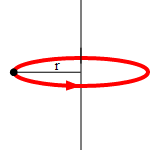
\includegraphics{./img/inertia.png}
\end{center}

Zaś dla ciałą składającego się z \emph{n} punktów moment bezwładności jest sumą
momentów bezwładności wszystkich punktów.
\begin{equation}
I = \sum_{i=1}^{n} m_{i}r_{i}^{2}
\end{equation}
Dla zaimplementowanych kształtów w omawianynej bibliotece obudowującej wartości
momentu bezwładności są następujące:\\
Dla kuli (\emph{sphere}):\\
\begin{center}
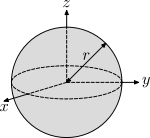
\includegraphics{./img/inertiaSphere.png}
\end{center}
\begin{equation}
I = \frac{2}{5}mr^{2}
\end{equation}
Dla prostopadłościanu (\emph{box}):\\
\begin{center}
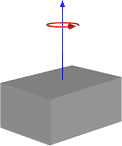
\includegraphics{./img/inertiaBox.png}
\end{center}
Dla dowolnej osi obrotu $ \hat{n} $ przechodzącej przez środek masy sześcianu
moment bezwładności jest określany przez następuące równanie:
\begin{equation}
I = m\hat{n}^{T}\hat{I}\hat{n} = m
\begin{bmatrix}n_{x}&n_{y}&n_{z}\end{bmatrix}
\begin{bmatrix}y^{2}+z^{2}&-xy&-xz\\-yx&x^{2}+z^{2}&-yz\\-zx&-zy&x^{2}+y^{2}\end{bmatrix}
\begin{bmatrix}n_{x}\\n_{y}\\n_{z}\end{bmatrix}
\label{eq:boxInertia}
\end{equation}
Gdzie:\\
$\hat{I}$ jest wartością tensora momentu bezwładności ciała.\\
Wartości $n_{x}$, $n_{y}$ i $n_{z}$ to składowe wektora $\hat{n}$.\\
Wartości \emph{x}, \emph{y} i \emph{z}, to kolejno szerokość, wysokość i długość
rozważanego prostopadłościanu.\\ \\
Nie jest konieczne implementowanie momentu bezwładności osobno dla każdego typu
bryły. Silnik bullet przechowuje wartość macierzy momentu bezwładności dla
każdego obiektu klasy \emph{btRigidBody}.

\lstinputlisting[language=c++, caption=fragment pliku
btRigidBody.h,
label=lis:RigidBodyh,linerange={55-60}]{./listings/btRigidBody.h}

Pole \emph{m\_invInertiaTensorWorld} zawiera odwrotną macierz momentu
bezwładności w odniesieniu do macierzy świata symulacji.

\lstinputlisting[language=c++, caption=fragment pliku
CollisionShape.cpp,
label=lis:CollisionShapecpp,linerange={162-168}]{./listings/CollisionShape.cpp}

W 6. linijce listingu \ref{lis:CollisionShapecpp} realizowane jest mnożenie wektorów
\emph{n} (transpozycja jest realizowana przez iloczyn skalarny (\emph{dot})
dwóch powstałych wektorów) z równaia \ref{eq:boxInertia}.

\lstinputlisting[language=java, caption=fragment pliku
CollisionShape.java,
label=lis:CollisionShapejava,linerange={38-38,142-145,
147-153}]{./listings/CollisionShape.java}

Ponieważ wyciągana wartość w kodzie natywnym to odwrotna wartość momentu
bezwładności, w linijce 4 zostaje ona sprowadzona do wartości prawidłowej. Jako
oś obrotu zostaje obrany znormalizowany wektor prędkości kątowej (ln. 10).\\


\textbf{Całkowita energia kinetyczna}\\
Podsumowując, dla testów w tej podsekcji sprawdzone zostanie czy spełniony
jest następujący warunek dla \emph{n} ciał:
\begin{equation}
E_{K} = \sum_{i=1}^{n}\left(\frac{mv^{2}}{2} + \frac{I\omega^{2}}{2}\right) =
const.
\end{equation}
Warunek jest sprawdzany przez metodę:
\lstinputlisting[language=java, caption=fragment
pliku CollisionShape.java,
label=lis:CollisionShapejava2,linerange={155-158}]{./listings/CollisionShape.java}


\textbf{Energia potencjalna}\\
Drugim rodzajem energii występującym w fizyce klasycznej jest energia
potencjalna. Jest to energia jaką posiada ciało za sprawą swojej pozycji i
pozycji innych ciał względem jego. Podobnie jak w przypadku energii
kinetycznej, rozważane będą dwa rodzaje energii potencjalnej: grawitacji i
sprężystości.\\

\textbf{Energia potencjalna grawitacji}\\
Energia ta jest wynikiem znajdowania się ciała w polu grawitacynym innych ciał.
Ogólnym wzorem na wyznaczenie jej wartości dla ciała o masie \emph{m}, przy
założeniu, że ciała mają kształt kuli to:

\begin{equation}
E_{P} = mG\sum_{i=1}^{n}\frac{m_{i}}{r_{i}}
\label{eq:epgravity}
\end{equation}
Gdzie:\\
\emph{G} to stała grawitacji.\\
$ m_{i} $ jest masą \emph{i}-tego ciała tworzącego pole grawitacyjne.\\
$ r_{i} $ to odległość badanego ciała od \emph{i}-tego ciała.\\

Zakładając że ciałem wytwarzającym pole grawitacyjne jest kula ziemska i że
przyspieszenie ziemskie \emph{g} wynosi $ GM_{Z} $ wzór
\ref{eq:epgravity} przyjmuje po uproszczeniu postać:

\begin{equation}
E_{P} = mgr_{Z}
\end{equation}
Gdzie $ r_{Z} $ to odległość środka ciała od środka Ziemi. Ponieważ podczas
testów istotne będą jedynie zmiany wartości energii potencjalnej:

\begin{equation}
\Delta E_{P} = mg\Delta h
\end{equation}

Do obliczenia wartości zostanie wykorzystana metoda klasy \emph{CollisionShape}.
Obraną ustaloną wysokością będzie współrzędna \emph{y} ciała.

\begin{lstlisting}[language=Java,
caption=fragment pliku CollisionShape.java,label=lis:epgravity]
float getGravitationalPotentialEnergy()
{
	return mass*9.81f*getTranslation().y;
}
\end{lstlisting}

\textbf{Energia potencjalna sprężystości}\\
Ten rodzaj energii jest właściwy dla ciał posiadających sprężystość. Pojawia się
gdy ciało zostaje odkształcone, a jej wartość jest proporcjonalna do siły
wymuszającej powrót do jego stabilnego stanu. Ogólnym wzorem wyznacząjącym
wartość tej energii dla sprężyny jest:

\begin{equation}
\Delta E_{P} = \frac{kx^{2}}{2}
\end{equation}
Gdzie:\\
\emph{k} to współczynnik sprężystości ciała.\\
\emph{x} jest odległością na jaką została odkształcona spręzyna.\\
 \\
Energia potencjalna spręzystości jest właściwa tylko dla ciał sprężystych,
dlatego zostaje zaimplementowana jedynie w klasie \emph{Spring}.

\begin{lstlisting}[language=Java,
caption=Obliczanie energii potencjalnej spręzystości,label=lis:epelastic]
public class Spring
{
	...
	
	private CollisionShape rb1, rb2;
	private Vector3 relation;
	private float stiffness;
	
	public Spring(DynamicsWorld dw, CollisionShape rb1, CollisionShape rb2, Vector3 frameA, Vector3 frameB, boolean linear)
	{
		id = constructor(dw.id, rb1.id, rb2.id, frameA, frameB, linear);
		this.rb1 = rb1;
		this.rb2 = rb2;
		relation = rb2.getTranslation().subtract(rb1.getTranslation());
	}
	
	public void setupDof(Dof index, float stiffness, float damping)
	{
		enable(index, true);
		setDamping(index, damping);
		setStiffness(index, stiffness);
		this.stiffness = stiffness;
	}
	
	public float getElasticPotentialEnergy()
	{
		Vector3 stablePos = relation.clone().rotate(rb1.getRotation()).add(rb1.getTranslation());
		float x = stablePos.subtract(rb2.getTranslation()).length();
		return (float)Math.pow(x, 2)*stiffness/2.0f;
	}
	
	...
}
\end{lstlisting}
Dane o ciałach \textbf{A} i \textbf{B} (o których była mowa w paragrafie
\ref{sec:spring}), przechowane są w momencie tworzenia obiektu przez konstruktor
(jako \emph{rb1} i \emph{rb2} ln. 12-13). Zachowany jest również wektor relacji
pozycji ciała \textbf{A} do ciała \textbf{B} (ln. 14), w celu określenia
stabilnej pozycji ciała \textbf{B}. Współczynnik sprężystości (w tym miejscu
oznaczony jako \emph{stiffness}) także jest zachowywany do póżniejszych obliczeń
(ln. 22). Wartość energii potencjalnej sprężystości jest zwracana przez metodę
\emph{getElasticPotentialEnergy}. Wektor \emph{stablePos} (ln. 27) jest stabilną
pozycją ciała \textbf{B} względem środka świata symulacji. Odległość między
\emph{stablePos} a pozycją ciała \textbf{B} stanowi miarę odkształcenia
\emph{x} (ln. 28).

\subsubsection{Odbicie sprężyste jednego ciała}\label{sec:odbicie1ciala}
Na początek zostanie rozważony najprostszy przypadek z jedną kulką
odbijającą się kolejno od dwóch idealnie sprężystych ścianek. Ponieważ w
testach wykonywanych w tej podsekcji nie są zakładane oddziaływania pomiędzy
ciałami, zostaną rozważone jedynie zmiany energii kinetycznej. Do tego testu
wykorzystana została scena prezentowana na listingu
\ref{lis:SimpleSnookerScene}. Test ma na celu zbadanie rzeczywistej zależności
zmian energii kinetycznej ciała przy odbiciach od jego współczynnika
sprężystośści.

\lstinputlisting[language=Java,
caption=scena testująca przypadek z jednym ciałem,
label=lis:SimpleSnookerScene]{./listings/SimpleSnookerScene.java}
Na niesprężystym (ln. 57) i całkowicie śliskim (ln. 55) podłożu zostaje
umieszczona kulka (ln. 59), która przez nadaną jej prędkość początkową (ln. 62)
odbija się kolejno od ścianek (ln. 49, 50). Sprężystość (\emph{restitution})
kulki jak i ścianek jest regulowana na początku każdego testu (ln. 73, 74),
która dla pierszego wynosi 0.9 (ln. 18) i jest liniowo zwiększana dla kolejnych
dziesięciu testów (ln. 21, 24, 94) aż do osiągnięcia wartości 1 (gdzie
teoretycznie energia kulki powinna być stała).
Dla każdej testowanej wartości przewidziano 20 odbić (ln. 22, 23, 81-97).
Energia kinetyczna kulki jest zapisywana do pliku przy każdym odbiciu (ln.
81-87).

\begin{center}
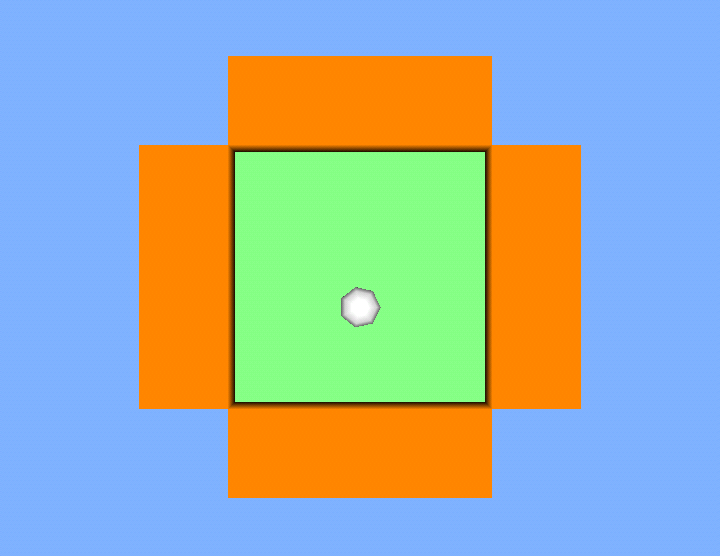
\includegraphics[scale = 0.5]{./img/SimpleSnookerScene.png}
\end{center}

Zależność energii kinetycznej kulki przy kolejnych jej odbiciach od wartości
sprężystości jest przedstawiona na poniższym wykresie.

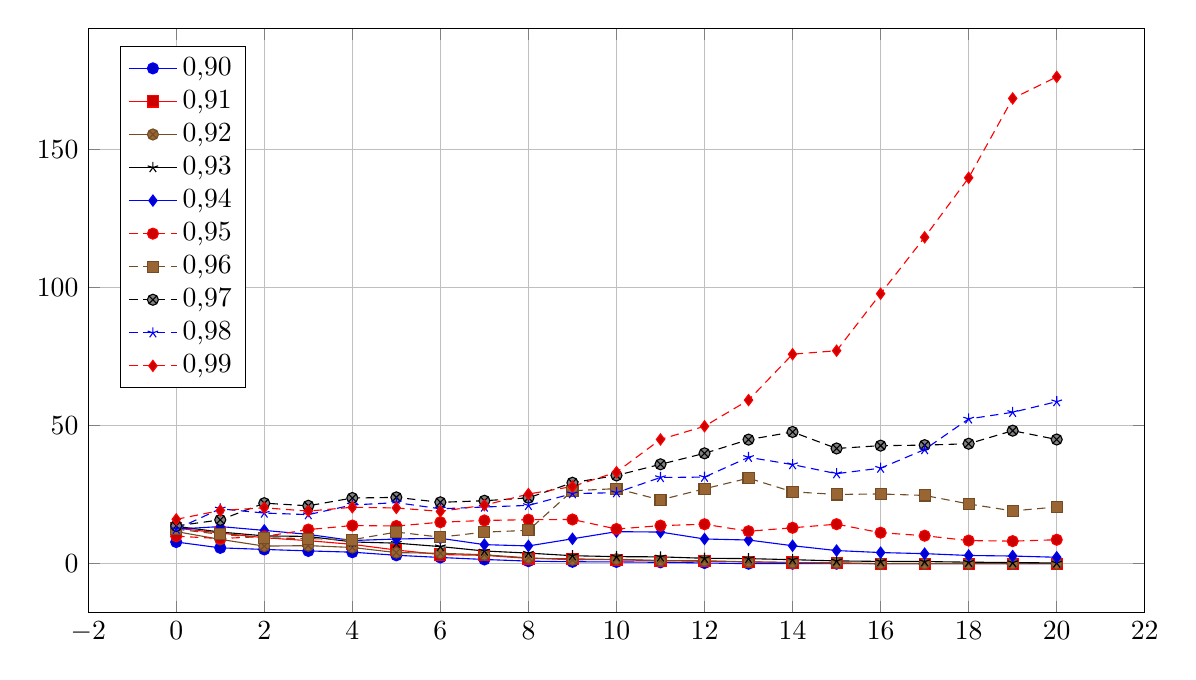
\begin{tikzpicture}
\begin{axis}[
height=9cm,
width=15cm,
grid=major,
legend style = { legend pos = north west }
]
\addplot coordinates {(0, 7.8372054) (1, 5.726038) (2, 5.154667) (3, 4.621181) (4, 4.1600547) (5, 3.0396576) (6, 2.239414) (7, 1.5242789) (8, 0.92045516) (9, 0.6885652) (10, 0.65223116) (11, 0.48610428) (12, 0.2598384) (13, 0.0) (14, 0.0) (15, 0.0) (16, 0.0) (17, 0.0) (18, 0.0) (19, 0.0) (20, 0.0) };
\addlegendentry{0,90}
\addplot coordinates {(0, 12.871898) (1, 11.081771) (2, 9.383892) (3, 8.331373) (4, 6.9849744) (5, 4.9359865) (6, 3.3015344) (7, 3.012378) (8, 1.8939176) (9, 1.7871089) (10, 1.3716524) (11, 1.1143106) (12, 0.8515529) (13, 0.6746103) (14, 0.39734042) (15, 0.20273632) (16, 0.0) (17, 0.0) (18, 0.0) (19, 0.0) (20, 0.0) };
\addlegendentry{0,91}
\addplot coordinates {(0, 11.617334) (1, 8.787009) (2, 6.3560305) (3, 6.531136) (4, 5.861786) (5, 4.0063114) (6, 3.7645807) (7, 3.226793) (8, 2.0987976) (9, 1.3800614) (10, 1.6246796) (11, 1.1037858) (12, 1.059758) (13, 0.6554112) (14, 0.39335263) (15, 0.31620935) (16, 0.0) (17, 0.0) (18, 0.0) (19, 0.0) (20, 0.0) };
\addlegendentry{0,92}
\addplot coordinates {(0, 13.517401) (1, 11.452294) (2, 10.057288) (3, 9.859059) (4, 7.8632793) (5, 7.422488) (6, 6.1805496) (7, 4.5945706) (8, 3.825597) (9, 2.8837724) (10, 2.5438883) (11, 2.4632976) (12, 1.957013) (13, 1.8278275) (14, 1.4445596) (15, 1.0002052) (16, 0.81805015) (17, 0.7711672) (18, 0.5411076) (19, 0.4110637) (20, 0.252428) };
\addlegendentry{0,93}
\addplot coordinates {(0, 12.5) (1, 13.43023) (2, 12.048469) (3, 10.599778) (4, 8.368018) (5, 8.931303) (6, 9.189003) (7, 6.895406) (8, 6.4192615) (9, 9.002274) (10, 11.5897455) (11, 11.443102) (12, 8.935459) (13, 8.56017) (14, 6.4986897) (15, 4.7467318) (16, 4.0223384) (17, 3.6290448) (18, 2.9679754) (19, 2.765107) (20, 2.318351) };
\addlegendentry{0,94}
\addplot coordinates {(0, 9.945217) (1, 9.09356) (2, 9.837457) (3, 12.346309) (4, 13.799155) (5, 13.630574) (6, 14.99853) (7, 15.637733) (8, 15.918938) (9, 15.996337) (10, 12.536006) (11, 13.770408) (12, 14.269985) (13, 11.742347) (14, 12.98971) (15, 14.293675) (16, 11.207167) (17, 10.119975) (18, 8.35863) (19, 8.154236) (20, 8.6633835) };
\addlegendentry{0,95}
\addplot coordinates {(0, 12.5) (1, 10.616831) (2, 9.379364) (3, 9.0645) (4, 8.673918) (5, 11.4384165) (6, 9.595471) (7, 11.418807) (8, 12.055469) (9, 26.387554) (10, 27.160097) (11, 23.074898) (12, 27.107899) (13, 30.953737) (14, 26.003126) (15, 25.055992) (16, 25.225168) (17, 24.703861) (18, 21.618656) (19, 19.09106) (20, 20.514286) };
\addlegendentry{0,96}
\addplot coordinates {(0, 13.680727) (1, 15.846518) (2, 21.887976) (3, 20.95167) (4, 23.759962) (5, 23.993092) (6, 22.206078) (7, 22.775206) (8, 23.825249) (9, 29.290152) (10, 31.927158) (11, 35.96635) (12, 39.931347) (13, 44.896645) (14, 47.657745) (15, 41.694195) (16, 42.71819) (17, 42.896385) (18, 43.41286) (19, 48.133793) (20, 44.937626) };
\addlegendentry{0,97}
\addplot coordinates {(0, 12.5) (1, 19.857609) (2, 18.324724) (3, 17.74957) (4, 21.24073) (5, 22.094864) (6, 19.864298) (7, 20.512543) (8, 21.093626) (9, 25.34785) (10, 25.709059) (11, 31.19894) (12, 31.330263) (13, 38.49805) (14, 35.860638) (15, 32.578533) (16, 34.57723) (17, 41.310635) (18, 52.382793) (19, 54.786243) (20, 58.630527) };
\addlegendentry{0,98}
\addplot coordinates {(0, 16.047285) (1, 19.260551) (2, 20.213194) (3, 19.034306) (4, 20.410967) (5, 20.158894) (6, 18.924496) (7, 21.155848) (8, 25.198473) (9, 27.927269) (10, 33.119106) (11, 44.98241) (12, 49.725594) (13, 59.206253) (14, 75.80497) (15, 77.06952) (16, 97.705864) (17, 118.11795) (18, 139.648) (19, 168.3767) (20, 176.16727) };
\addlegendentry{0,99}
\end{axis}
\end{tikzpicture}



Jak widać w doświadczeniu nie osiągnięto spodziewanych rezultatów. Dla
sprężystości o wartości 1 energia kinetyczna powinna być stała, natomiast tutaj
gwałtownie wzrasta. Wydaje się, że dla utrzymania stałej energii kinetycznej
konieczne jest użycie niższej wartości. Dla polepszenia widoczności poniższy
wykres zawiera wartości energii kinetycznej dla wartości sprężystości od 0,94 do
0,97.

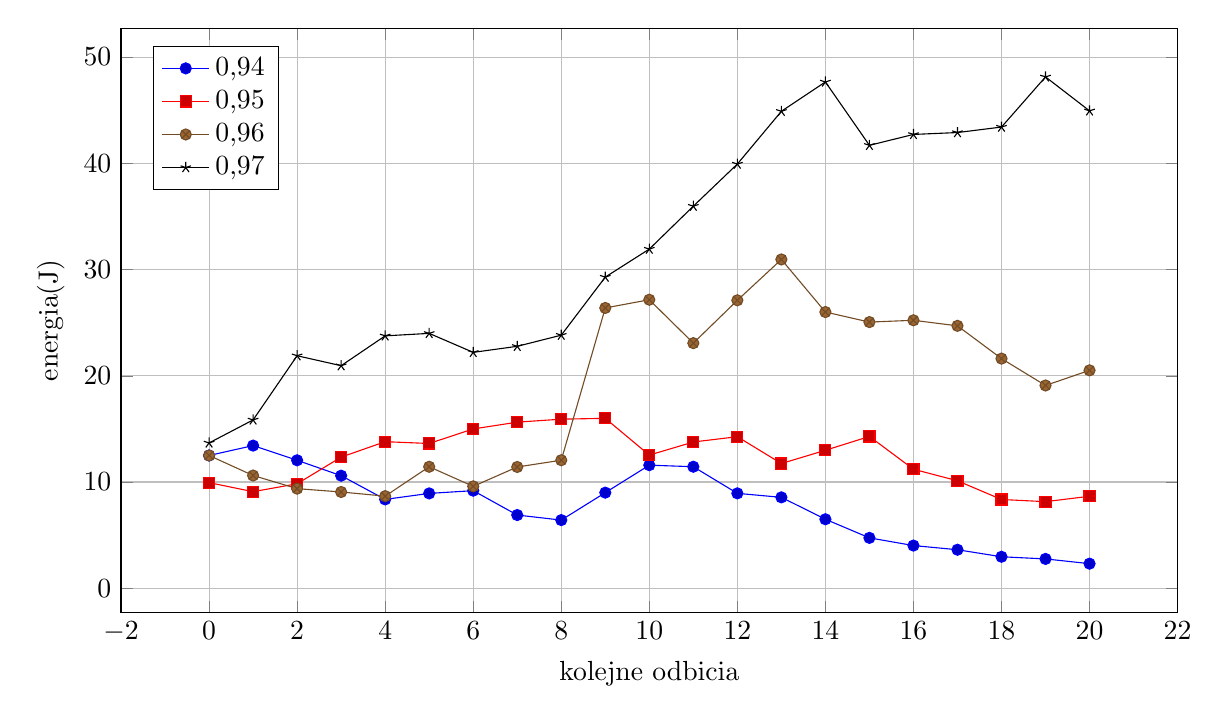
\begin{tikzpicture}
\begin{axis}[
height=9cm,
width=15cm,
grid=major,
xlabel=kolejne odbicia,
ylabel=energia(J),
legend style = { legend pos = north west }
]
\addplot coordinates {(0, 12.5) (1, 13.43023) (2, 12.048469) (3, 10.599778) (4,8.368018) (5, 8.931303) (6, 9.189003) (7, 6.895406) (8, 6.4192615) (9, 9.002274) (10, 11.5897455) (11, 11.443102) (12, 8.935459) (13, 8.56017) (14, 6.4986897) (15, 4.7467318) (16, 4.0223384) (17, 3.6290448) (18, 2.9679754) (19, 2.765107) (20, 2.318351) };
\addlegendentry{0,94}
\addplot coordinates {(0, 9.945217) (1, 9.09356) (2, 9.837457) (3, 12.346309) (4, 13.799155) (5, 13.630574) (6, 14.99853) (7, 15.637733) (8, 15.918938) (9, 15.996337) (10, 12.536006) (11, 13.770408) (12, 14.269985) (13, 11.742347) (14, 12.98971) (15, 14.293675) (16, 11.207167) (17, 10.119975) (18, 8.35863) (19, 8.154236) (20, 8.6633835) };
\addlegendentry{0,95}
\addplot coordinates {(0, 12.5) (1, 10.616831) (2, 9.379364) (3, 9.0645) (4, 8.673918) (5, 11.4384165) (6, 9.595471) (7, 11.418807) (8, 12.055469) (9, 26.387554) (10, 27.160097) (11, 23.074898) (12, 27.107899) (13, 30.953737) (14, 26.003126) (15, 25.055992) (16, 25.225168) (17, 24.703861) (18, 21.618656) (19, 19.09106) (20, 20.514286) };
\addlegendentry{0,96}
\addplot coordinates {(0, 13.680727) (1, 15.846518) (2, 21.887976) (3, 20.95167) (4, 23.759962) (5, 23.993092) (6, 22.206078) (7, 22.775206) (8, 23.825249) (9, 29.290152) (10, 31.927158) (11, 35.96635) (12, 39.931347) (13, 44.896645) (14, 47.657745) (15, 41.694195) (16, 42.71819) (17, 42.896385) (18, 43.41286) (19, 48.133793) (20, 44.937626) };
\addlegendentry{0,97}
\end{axis}
\end{tikzpicture}



Przy początkowej prędkości 5$\frac{m}{s}$ i masie 1 kg (listing
\ref{lis:SimpleSnookerScene} ln. 72, 59) energia kinetyczna kulki powinna mieć
stałą wartość energii kinetycznej 12,5.
\begin{equation}
E_{K} = \frac{mv^{2}}{2} = \frac{1kg*(5\frac{m}{s})^{2}}{2} =
12,5J
\end{equation}
Z prezentowanego wykresu wynika, że najbardziej odpowiednia wartość
współczynnika sprężystości kulki i ścianek mieści się między 0,945 a 0,955.\\
Dla ustalenia bardziej szczegółowej wartości test został powtórzony dla
następujących parametrów z listingu \ref{lis:SimpleSnookerScene}:

\lstinputlisting[language=Java,
  label=lis:SimpleSnookerScene_additional]{./listings/SimpleSnookerScene_additional.java}
  
Ilość odbić została zwiększona dwukrotnie, dzięki czemu możliwe jest sprawdzenie
czy wyrównany poziom energii będzie się utrzymywać.
  
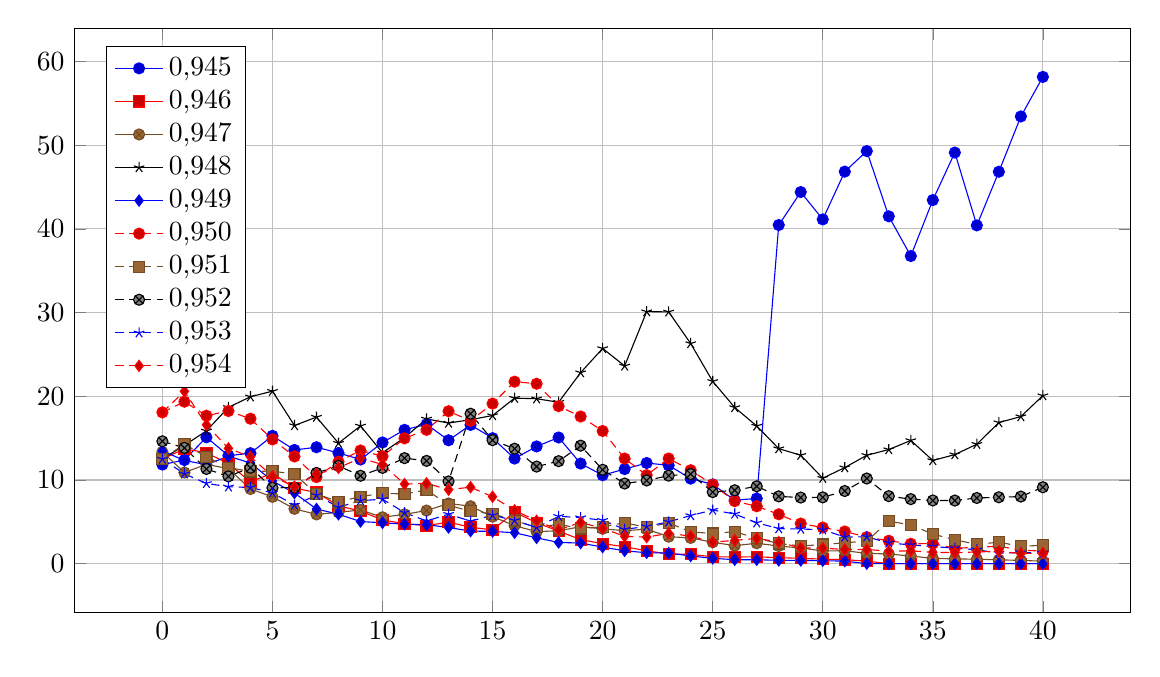
\begin{tikzpicture}
\begin{axis}[
height=9cm,
width=15cm,
grid=major,
legend style = { legend pos = north west }
]
\addplot coordinates {(0, 11.83472) (1, 12.379627) (2, 15.0980625) (3, 12.897377) (4, 13.197653) (5, 15.268386) (6, 13.5835) (7, 13.907026) (8, 13.226399) (9, 12.440128) (10, 14.477035) (11, 15.9842) (12, 16.644344) (13, 14.740385) (14, 16.573435) (15, 14.992984) (16, 12.555236) (17, 14.004993) (18, 15.072159) (19, 11.958659) (20, 10.568625) (21, 11.297269) (22, 12.023627) (23, 11.743839) (24, 10.15784) (25, 9.469015) (26, 7.5816555) (27, 7.7853804) (28, 40.450466) (29, 44.389053) (30, 41.125744) (31, 46.831127) (32, 49.287273) (33, 41.49332) (34, 36.746765) (35, 43.43231) (36, 49.10869) (37, 40.409218) (38, 46.817432) (39, 53.422592) (40, 58.14726) };
\addlegendentry{0,945}
\addplot coordinates {(0, 12.5) (1, 13.725066) (2, 13.244118) (3, 11.953949) (4, 9.769774) (5, 10.814914) (6, 9.028812) (7, 8.502626) (8, 6.9107122) (9, 6.27938) (10, 5.2203937) (11, 4.7625675) (12, 4.5451007) (13, 4.9654703) (14, 4.347088) (15, 4.030155) (16, 6.161413) (17, 4.8873606) (18, 3.8916974) (19, 2.8733) (20, 2.3946586) (21, 2.0231962) (22, 1.533896) (23, 1.1654351) (24, 1.111763) (25, 0.82033926) (26, 0.7949642) (27, 0.81605846) (28, 0.7132569) (29, 0.63949037) (30, 0.5374603) (31, 0.4743589) (32, 0.297938) (33, 0.0) (34, 0.0) (35, 0.0) (36, 0.0) (37, 0.0) (38, 0.0) (39, 0.0) (40, 0.0) };
\addlegendentry{0,946}
\addplot coordinates {(0, 13.343076) (1, 10.882678) (2, 11.869106) (3, 11.345713) (4, 8.922309) (5, 7.9773874) (6, 6.547513) (7, 5.882253) (8, 6.130847) (9, 6.4155216) (10, 5.5394745) (11, 5.896995) (12, 6.3431163) (13, 7.1916647) (14, 6.862142) (15, 5.6141715) (16, 4.546112) (17, 3.814531) (18, 3.9349108) (19, 4.4040594) (20, 4.1672707) (21, 3.9381962) (22, 4.1216965) (23, 3.2221136) (24, 3.074441) (25, 2.554985) (26, 2.152308) (27, 2.4376867) (28, 2.1064556) (29, 1.8707508) (30, 1.5296999) (31, 1.5388436) (32, 1.2382075) (33, 1.149339) (34, 0.91256565) (35, 0.63522154) (36, 0.56922203) (37, 0.5338146) (38, 0.45862925) (39, 0.38885325) (40, 0.2969072) };
\addlegendentry{0,947}
\addplot coordinates {(0, 12.5) (1, 14.13552) (2, 15.8612585) (3, 18.670893) (4, 19.937475) (5, 20.604156) (6, 16.50161) (7, 17.508545) (8, 14.396487) (9, 16.455772) (10, 13.244559) (11, 15.055199) (12, 17.29025) (13, 16.797775) (14, 17.200518) (15, 17.697063) (16, 19.771584) (17, 19.701103) (18, 19.285048) (19, 22.817455) (20, 25.708588) (21, 23.621098) (22, 30.10682) (23, 30.076248) (24, 26.296255) (25, 21.77965) (26, 18.656929) (27, 16.446127) (28, 13.739975) (29, 12.953177) (30, 10.209646) (31, 11.477742) (32, 12.947726) (33, 13.629319) (34, 14.718304) (35, 12.328139) (36, 13.029368) (37, 14.271083) (38, 16.854652) (39, 17.572474) (40, 20.073355) };
\addlegendentry{0,948}
\addplot coordinates {(0, 13.470681) (1, 12.325375) (2, 11.826186) (3, 12.835963) (4, 12.031693) (5, 9.875669) (6, 8.433987) (7, 6.5284123) (8, 5.901152) (9, 5.0297904) (10, 4.8878074) (11, 4.7115064) (12, 4.658539) (13, 4.315971) (14, 3.8937955) (15, 3.852501) (16, 3.6964788) (17, 3.084705) (18, 2.5341594) (19, 2.460717) (20, 1.9807745) (21, 1.5402061) (22, 1.3024533) (23, 1.2666614) (24, 0.92073756) (25, 0.6371743) (26, 0.47197518) (27, 0.4704443) (28, 0.39559248) (29, 0.38954863) (30, 0.35554305) (31, 0.29937363) (32, 0.0) (33, 0.0) (34, 0.0) (35, 0.0) (36, 0.0) (37, 0.0) (38, 0.0) (39, 0.0) (40, 0.0) };
\addlegendentry{0,949}
\addplot coordinates {(0, 18.075089) (1, 19.348585) (2, 17.674715) (3, 18.23503) (4, 17.312439) (5, 14.840965) (6, 12.803486) (7, 10.340366) (8, 12.173147) (9, 13.52262) (10, 12.823664) (11, 14.969939) (12, 15.979581) (13, 18.209831) (14, 17.077518) (15, 19.11712) (16, 21.73974) (17, 21.490181) (18, 18.81594) (19, 17.580912) (20, 15.849103) (21, 12.554693) (22, 10.572047) (23, 12.559721) (24, 11.165561) (25, 9.431433) (26, 7.4705954) (27, 6.854054) (28, 5.899695) (29, 4.790389) (30, 4.3167667) (31, 3.8425434) (32, 3.17302) (33, 2.7332091) (34, 2.3748143) (35, 2.3970597) (36, 1.84973) (37, 1.9432095) (38, 2.087145) (39, 1.6142488) (40, 1.4980283) };
\addlegendentry{0,950}
\addplot coordinates {(0, 12.5) (1, 14.287379) (2, 12.751261) (3, 11.474439) (4, 11.014549) (5, 11.059993) (6, 10.678994) (7, 8.348292) (8, 7.3942523) (9, 8.00856) (10, 8.404354) (11, 8.3236065) (12, 8.814266) (13, 6.9876337) (14, 6.250312) (15, 5.9692373) (16, 5.1552496) (17, 4.34337) (18, 4.697723) (19, 4.2021036) (20, 4.4029956) (21, 4.88272) (22, 4.3309884) (23, 4.8590584) (24, 3.806094) (25, 3.5954096) (26, 3.8256135) (27, 3.019442) (28, 2.412923) (29, 2.1122441) (30, 2.2830546) (31, 2.4955637) (32, 2.6976843) (33, 5.0676746) (34, 4.630739) (35, 3.531819) (36, 2.855678) (37, 2.2971077) (38, 2.5723886) (39, 2.0594285) (40, 2.205233) };
\addlegendentry{0,951}
\addplot coordinates {(0, 14.615244) (1, 13.829683) (2, 11.311698) (3, 10.427009) (4, 11.460272) (5, 9.057038) (6, 9.099048) (7, 10.840954) (8, 11.678121) (9, 10.499791) (10, 11.441355) (11, 12.603779) (12, 12.279609) (13, 9.823079) (14, 17.913473) (15, 14.754623) (16, 13.729808) (17, 11.595872) (18, 12.243206) (19, 14.099075) (20, 11.214356) (21, 9.572169) (22, 9.937819) (23, 10.514322) (24, 10.702424) (25, 8.548818) (26, 8.768956) (27, 9.24096) (28, 8.037726) (29, 7.8958397) (30, 7.919593) (31, 8.676345) (32, 10.173832) (33, 8.067685) (34, 7.7079425) (35, 7.548844) (36, 7.5379424) (37, 7.846434) (38, 7.9307866) (39, 8.014059) (40, 9.130319) };
\addlegendentry{0,952}
\addplot coordinates {(0, 12.5) (1, 10.7275) (2, 9.595271) (3, 9.179574) (4, 9.106409) (5, 8.454757) (6, 7.0024796) (7, 8.17677) (8, 6.750139) (9, 7.5269756) (10, 7.698658) (11, 6.103392) (12, 5.0972943) (13, 5.914313) (14, 5.076894) (15, 5.787914) (16, 5.162111) (17, 4.3161173) (18, 5.6562753) (19, 5.5016747) (20, 5.1850286) (21, 4.1028576) (22, 4.4445443) (23, 4.9968286) (24, 5.750374) (25, 6.4052725) (26, 5.936255) (27, 4.8863425) (28, 4.1847186) (29, 4.1409235) (30, 4.0526757) (31, 3.1830995) (32, 3.1974099) (33, 2.4858365) (34, 2.2343047) (35, 2.0511215) (36, 1.8490995) (37, 1.6669159) (38, 1.2392174) (39, 1.3421869) (40, 1.2746574) };
\addlegendentry{0,953}
\addplot coordinates {(0, 18.07279) (1, 20.592321) (2, 16.581625) (3, 13.767898) (4, 12.763923) (5, 10.439662) (6, 9.18948) (7, 10.687139) (8, 11.447489) (9, 12.615019) (10, 11.8371315) (11, 9.515284) (12, 9.591186) (13, 8.840663) (14, 9.133119) (15, 7.9945536) (16, 6.3630214) (17, 5.123591) (18, 4.040571) (19, 4.926172) (20, 4.223811) (21, 3.267189) (22, 3.1675262) (23, 3.6172326) (24, 3.2864053) (25, 2.576568) (26, 2.7800326) (27, 3.020876) (28, 2.5800412) (29, 1.8733292) (30, 1.85761) (31, 1.6878184) (32, 1.7023418) (33, 1.4894247) (34, 1.5277467) (35, 1.3547096) (36, 1.3137895) (37, 1.3966576) (38, 1.4822598) (39, 1.2024833) (40, 1.2677329) };
\addlegendentry{0,954}
\end{axis}
\end{tikzpicture}

Jak widać poziom energii nie utrzymuje się dla zwiększonej ilości odbić. W
dodatku w losowych momentach (na prezentowanym wykresie dla wartości
współczynnika sprężystości 0,945 dla 27. odbicia) można zaobserwować jego
gwałtowne wzrosty. Dla złagodzenia efektów tych wzrostów na poniższym wykresie
przedstawiono uśredniony wynik dziesięciu testów.

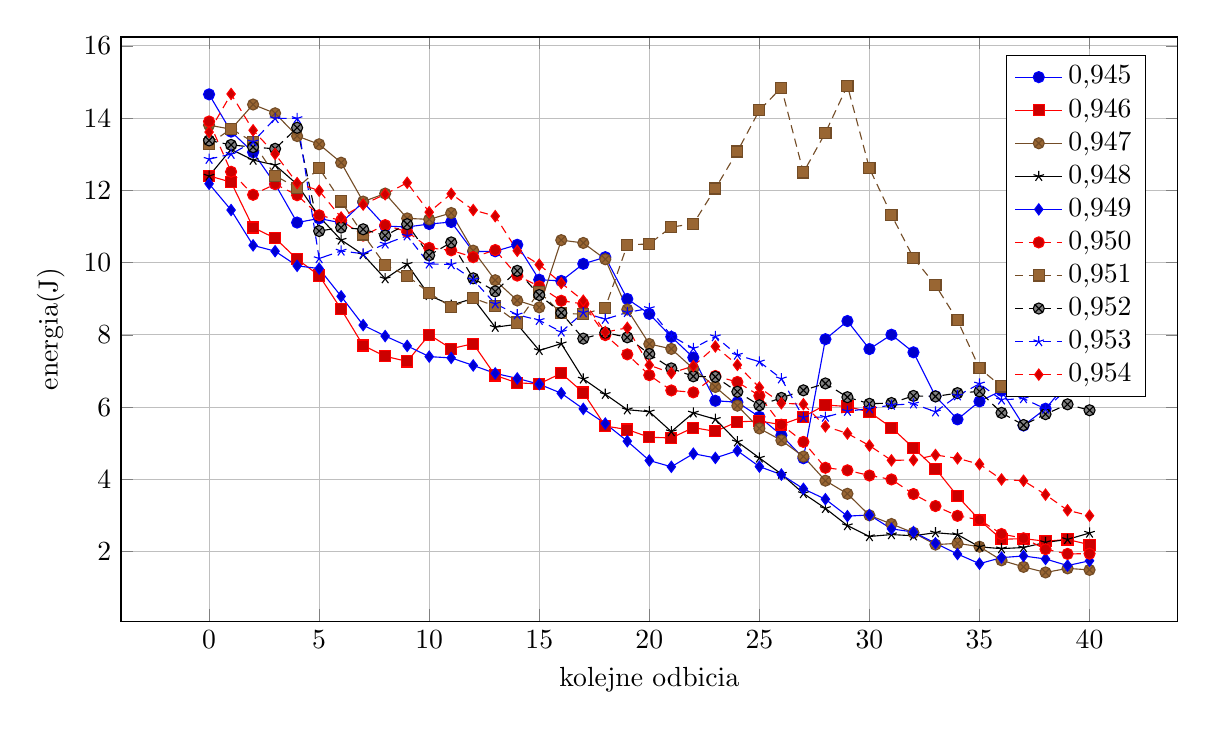
\begin{tikzpicture}
\begin{axis}[
height=9cm,
width=15cm,
grid=major,
xlabel=kolejne odbicia,
ylabel=energia(J),
legend style = { legend pos = north east }
]
\addplot coordinates {(0, 14.6562260627747) (1, 13.6256645202637) (2, 13.054486989975) (3, 12.1763894557953) (4, 11.108833360672) (5, 11.2233946323395) (6, 11.0991048336029) (7, 11.6744068145752) (8, 11.0118092298508) (9, 10.9873273611069) (10, 11.0685114145279) (11, 11.1239978551865) (12, 10.3053623557091) (13, 10.3141089200974) (14, 10.4938254594803) (15, 9.52750028371811) (16, 9.49386215209961) (17, 9.96602758169174) (18, 10.1507727026939) (19, 8.99497901201248) (20, 8.58136545419693) (21, 7.94662589430809) (22, 7.37444679141045) (23, 6.17753539681435) (24, 6.13745829164982) (25, 5.73345747590065) (26, 5.22426048517227) (27, 4.58836826682091) (28, 7.8813433110714) (29, 8.38399687707424) (30, 7.6084086805582) (31, 8.00572631806135) (32, 7.51851252317429) (33, 6.30226357579231) (34, 5.66303240656853) (35, 6.16019782423973) (36, 6.45491213798523) (37, 5.49251633584499) (38, 5.9576107352972) (39, 6.67393660545349) (40, 6.9803785264492) };
\addlegendentry{0,945}
\addplot coordinates {(0, 12.4022218704224) (1, 12.2259508132935) (2, 10.9725129127502) (3, 10.6760525226593) (4, 10.0991243362427) (5, 9.64306182861328) (6, 8.71197805404663) (7, 7.70718474388123) (8, 7.40868282318115) (9, 7.26591448783874) (10, 8.00451288223267) (11, 7.62072007656097) (12, 7.75652910470963) (13, 6.87890261411667) (14, 6.672678399086) (15, 6.64590454101563) (16, 6.93818979263306) (17, 6.40504869222641) (18, 5.47706761956215) (19, 5.38112026453018) (20, 5.16761724352837) (21, 5.14959081411362) (22, 5.43434517979622) (23, 5.33113816380501) (24, 5.59545066356659) (25, 5.61735334992409) (26, 5.51616925597191) (27, 5.73644617795944) (28, 6.06001359522343) (29, 6.01864603757858) (30, 5.86524453163147) (31, 5.43487996459007) (32, 4.8719010040164) (33, 4.30030767023563) (34, 3.53826675415039) (35, 2.87623463273048) (36, 2.34437598586082) (37, 2.36291944980621) (38, 2.29072198867798) (39, 2.33935695886612) (40, 2.19480673074722) };
\addlegendentry{0,946}
\addplot coordinates {(0, 13.8043006896973) (1, 13.6925736427307) (2, 14.3758071422577) (3, 14.1325853347778) (4, 13.5025720119476) (5, 13.2755349636078) (6, 12.7663237094879) (7, 11.6888662338257) (8, 11.9123019456863) (9, 11.2239685535431) (10, 11.1973436832428) (11, 11.3732707977295) (12, 10.3317072629929) (13, 9.51320831775665) (14, 8.95262567996979) (15, 8.76283481121063) (16, 10.6224771022797) (17, 10.5448018312454) (18, 10.0935352087021) (19, 8.7033514380455) (20, 7.7492377281189) (21, 7.61283913850784) (22, 7.06518988609314) (23, 6.559628033638) (24, 6.04167060852051) (25, 5.41185646653175) (26, 5.08241978287697) (27, 4.63394111096859) (28, 3.96660267710686) (29, 3.60402843356133) (30, 3.00693404078484) (31, 2.76765021979809) (32, 2.52679316997528) (33, 2.19694601595402) (34, 2.23208404928446) (35, 2.13959696292877) (36, 1.76221565306187) (37, 1.58085741400719) (38, 1.42672650814056) (39, 1.53932392001152) (40, 1.49729729890823) };
\addlegendentry{0,947}
\addplot coordinates {(0, 12.3982768058777) (1, 13.1348707199097) (2, 12.8372737884521) (3, 12.7001321792603) (4, 12.1672739028931) (5, 11.2750558376312) (6, 10.6261374473572) (7, 10.221337556839) (8, 9.55598180294037) (9, 9.95648241043091) (10, 9.09451639652252) (11, 8.82288656234741) (12, 9.00808305740356) (13, 8.21335928440094) (14, 8.29480786323547) (15, 7.57112445831299) (16, 7.75750745534897) (17, 6.78246188163757) (18, 6.35715628862381) (19, 5.93029171228409) (20, 5.87394794225693) (21, 5.32377170324326) (22, 5.8426962852478) (23, 5.66730691492558) (24, 5.04262288212776) (25, 4.59558297395706) (26, 4.14988817870617) (27, 3.61246277689934) (28, 3.19977921843529) (29, 2.72453445792198) (30, 2.42193761765957) (31, 2.47530001997948) (32, 2.44172253012657) (33, 2.52722045183182) (34, 2.47533693313599) (35, 2.13422930836678) (36, 2.08558965623379) (37, 2.11694244146347) (38, 2.25741191506386) (39, 2.34004321694374) (40, 2.51835238933563) };
\addlegendentry{0,948}
\addplot coordinates {(0, 12.1814444541931) (1, 11.4556957244873) (2, 10.4778209686279) (3, 10.3164783477783) (4, 9.91166429519653) (5, 9.83501195907593) (6, 9.06741237640381) (7, 8.27128520011902) (8, 7.96847171783447) (9, 7.6957754611969) (10, 7.39932823181152) (11, 7.36326403617859) (12, 7.15495343208313) (13, 6.93551654815674) (14, 6.79657573699951) (15, 6.63643126487732) (16, 6.38545722961426) (17, 5.95384972095489) (18, 5.54752365350723) (19, 5.0591068983078) (20, 4.52486710548401) (21, 4.35102623701096) (22, 4.71317600607872) (23, 4.59588846564293) (24, 4.79488226175308) (25, 4.35584520101547) (26, 4.1336768835783) (27, 3.74193927943706) (28, 3.45298179388046) (29, 2.98590224385262) (30, 3.01562243700027) (31, 2.63291162550449) (32, 2.54467267990112) (33, 2.23404234349728) (34, 1.9367674946785) (35, 1.66969993859529) (36, 1.83733677864075) (37, 1.88249142169952) (38, 1.79945760965347) (39, 1.61711151599884) (40, 1.74928727149963) };
\addlegendentry{0,949}
\addplot coordinates {(0, 13.9059829711914) (1, 12.5137694358826) (2, 11.8774974822998) (3, 12.1741494178772) (4, 11.8651987075806) (5, 11.310263633728) (6, 11.1685515403748) (7, 10.7494470119476) (8, 11.0378528118134) (9, 10.8539872646332) (10, 10.4069371700287) (11, 10.339888048172) (12, 10.1519442081451) (13, 10.3484754562378) (14, 9.64128794670105) (15, 9.3442617893219) (16, 8.94458522796631) (17, 8.85833351612091) (18, 7.99419071674347) (19, 7.46127936840057) (20, 6.88672922849655) (21, 6.46321547031403) (22, 6.40967074632645) (23, 6.86291975975037) (24, 6.69745423793793) (25, 6.31787598729134) (26, 5.51692352890968) (27, 5.03974458575249) (28, 4.32343353331089) (29, 4.25268172323704) (30, 4.10942476689816) (31, 4.00075962543488) (32, 3.59627936184406) (33, 3.26424064040184) (34, 2.99327031373978) (35, 2.88445642590523) (36, 2.49013569056988) (37, 2.37197640538216) (38, 2.06999402344227) (39, 1.94008515179157) (40, 1.94661874473095) };
\addlegendentry{0,950}
\addplot coordinates {(0, 13.2781973838806) (1, 13.7021299362183) (2, 13.3391201972961) (3, 12.4054169178009) (4, 12.0662398815155) (5, 12.6113337993622) (6, 11.6933528900146) (7, 10.780289888382) (8, 9.93317956924438) (9, 9.63696854114533) (10, 9.15944323539734) (11, 8.77189693450928) (12, 9.0159517288208) (13, 8.79784791469574) (14, 8.34251778125763) (15, 9.19578952789307) (16, 8.59856331348419) (17, 8.57238194942474) (18, 8.753364610672) (19, 10.4900251150131) (20, 10.5187027931213) (21, 10.9836204528809) (22, 11.075525021553) (23, 12.0515645503998) (24, 13.0754309654236) (25, 14.2149050116539) (26, 14.8429864764214) (27, 12.4947864532471) (28, 13.5947657942772) (29, 14.8968303561211) (30, 12.6081966876984) (31, 11.3213147640228) (32, 10.1299663484097) (33, 9.37871618270874) (34, 8.40511998534203) (35, 7.07489039599895) (36, 6.57302742898464) (37, 6.92401961386204) (38, 7.54064406454563) (39, 6.66278366148472) (40, 8.08269311785698) };
\addlegendentry{0,951}
\addplot coordinates {(0, 13.3815976142883) (1, 13.2575705528259) (2,13.1966584205627) (3, 13.1495709896088) (4, 13.7313847064972) (5, 10.8742453098297) (6, 10.9705602645874) (7, 10.9229876279831) (8, 10.7496512889862) (9, 11.0642107725143) (10, 10.2030373573303) (11, 10.5597208023071) (12, 9.56631820201874) (13, 9.204722905159) (14, 9.77342791557312) (15, 9.10343494415283) (16, 8.61196794509888) (17, 7.89711513519287) (18, 8.06343204975128) (19, 7.93230175971985) (20, 7.47169940471649) (21, 7.07361674308777) (22, 6.85348105430603) (23, 6.83944536447525) (24, 6.42703374624252) (25, 6.05213391780853) (26, 6.25701947212219) (27, 6.46634848117828) (28, 6.65723429918289) (29, 6.27693936228752) (30, 6.09445922374725) (31, 6.11582781076431) (32, 6.31241797208786) (33, 6.2971722304821) (34, 6.38925131559372) (35, 6.43648965060711) (36, 5.84381370544434) (37, 5.5056351006031) (38, 5.80657843947411) (39, 6.07883229255676) (40, 5.91480894088745) };
\addlegendentry{0,952}
\addplot coordinates {(0, 12.8636241912842) (1, 13.0021504402161) (2,
13.3448638916016) (3, 13.9903785705566) (4, 13.9917116641998) (5,
10.1146651744843) (6, 10.3231254577637) (7, 10.2456952095032) (8, 10.5174011230469) (9, 10.7428637504578) (10, 9.96562452316284) (11, 9.94694910049438) (12, 9.52446849346161) (13, 8.86221284866333) (14, 8.55821604728699) (15, 8.40437412261963) (16, 8.08280463218689) (17, 8.61760497093201) (18, 8.43606390953064) (19, 8.62183849811554) (20, 8.73446414470673) (21, 7.97404136657715) (22, 7.62777805328369) (23, 7.95511655807495) (24, 7.44362692832947) (25, 7.25623573064804) (26, 6.7876464009285) (27, 5.71654962301254) (28, 5.7262363910675) (29, 5.88920958042145) (30, 5.95987671017647) (31, 6.05756386518478) (32, 6.09318507313728) (33, 5.87254739105701) (34, 6.31689597964287) (35, 6.6472687035799) (36, 6.20203223526478) (37, 6.23965192735195) (38, 5.95067174732685) (39, 6.51158805936575) (40, 7.11151877641678) };
\addlegendentry{0,953}
\addplot coordinates {(0, 13.6133923530579) (1, 14.6667778968811) (2, 13.6618516921997) (3, 13.0073251724243) (4, 12.2023746013641) (5, 11.9906059265137) (6, 11.2490232944489) (7, 11.6071300029755) (8, 11.8916132926941) (9, 12.2103487968445) (10, 11.3969748973846) (11, 11.9060091018677) (12, 11.4559844017029) (13, 11.2876661777496) (14, 10.3291625261307) (15, 9.94409117698669) (16, 9.43445086479187) (17, 8.94726392030716) (18, 8.0772367477417) (19, 8.19570999145508) (20, 7.16313669681549) (21, 6.94529861211777) (22, 7.13770437240601) (23, 7.67992736101151) (24, 7.16948624849319) (25, 6.5456313252449) (26, 6.10883691906929) (27, 6.082444190979) (28, 5.47121298313141) (29, 5.27222081124783) (30, 4.93714967370033) (31, 4.5299041301012) (32, 4.53709046840668) (33, 4.67730629444122) (34, 4.58505046367645) (35, 4.42233805656433) (36, 4.00028142035007) (37, 3.96476039290428) (38, 3.58045221269131) (39, 3.14697138667107) (40, 2.99718299508095) };
\addlegendentry{0,954}
\end{axis}
\end{tikzpicture}


Spadki wartości energii kinetycznych sugerują, że nawet przy początkowo dobrze
dobranych współczynnikach sprężystości, przy większej ilości odbić energia nie
utrzymuje stałej wartości. Przy wartości współczynnika równej jedności energia
nie utrzymuje stałej wartości, a wzrasta. Co jest tego przyczyną? \\
W poszukiwaniu odpowiedzi na to pytanie można spojrzeć na wyniki poprzednich
testów rozpatrując osobno zapisy energii kinetycznej liniowej i obrotowej.
Poniżej przedstawiono fragment zapisu dla testu przy watrości współczynnika
sprężystości 0,98 (wartości energi liniowej energii kinetycznej znajdują się
po lewej stronie, a obrotowej po lewej):

\lstinputlisting[language=xml, caption=wartości energii kinetycznej,
  label=lis:linearAngle,linerange={6-12}]{./listings/0,98.txt}

Okazuje się, że nawet na całkowicie śliskim podłożu ciało uzyskuje obrotową
energię kinetyczną, co nie powinno mieć miejsca. Występowanie obrotu nie jest
jednak spowodowane tarciem ciała o podłoże, a wynikiem błędów zaokrągleń
kalkulacji silnika przy zderzeniach kulki ze ściankami.\\
Na listingu \ref{lis:linearAngle} można zaobserwować gwałtowne zmiany obu
energii, jednak wzrost energii kinetycznej liniowej jest zawsze poprzedzony
wzrostem energii kinetycznej obrotowej. Liniowa energia kinetyczna sama w sobie
nie ulega gwałtownym wzrostom. Przyczyną tego jest wzrost energii całkowitej.\\
Podczas analitycznego rozważania odbicia ciała możliwe jest dokładne ustalenie
czasu i miejsca zderzenia poprzez rozwiązanie odpowiedniego równania ruchu. W
przypadku symulacji zderzenia ciał przez silnik fizyczny, symulacja ta jest
dzielona na kroki. Każdy krok odpowiada minięciu kwantu czasu o z góry ustalonej
wartości i wszystkie ciała uczestniczące w symulacji poruszają się adekwatnie do
swojej prędkości. Prawie niemożliwe jest więc uzyskanie sytuacji w której
zderzenie powierzchni sferycznej z płaską będzie tylko jednym punktem.

\begin{center}
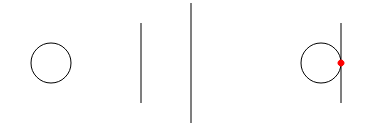
\includegraphics{./img/zderzenie1.png}
\end{center}

W przypadku zderzenia w symulacji zderzenie nie jest punktem a powierzchnią.
Silnik Bullet do obliczenia parametrów reakcji na zderzenie potrzebuje
określenia obszaru zderzenia jako punktu (który jest wybrany z powierzchni
obszaru zderzenia oznaczonego na poniższej ilustracji czerwoną linią). Niestety
im większy jest obszar zderzenia tym większe jest prawdopodobieństwo błędu w
wyborze odpowiedniego punktu. Przesunięcie tego punktu względem właściwego
umiejscowienia pozycji zderzenia wynikające z niedokładności obliczeniowej
decyduje o nadmiarze lub niedoborze obrotowej energii kinetycznej.

\begin{center}
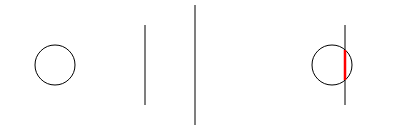
\includegraphics{./img/zderzenie2.png}
\end{center}

Aby zminimalizować możliwą wielkość obszaru zderzenia można zmniejszyć kwant
czasu, minimalizując odległości przebywane przez ciała w każdym kroku
symulacji.\\
Aby tego dokonać należy przyjrzeć się prototypowi funkcji \emph{stepSimulation}.

\lstinputlisting[language=c++,
label=lis:stepSimulation]{./listings/stepSimulation.cpp}

Funkcja ta jest wywoływana w celu zaktualizowania symulacji o pewien
czas (wywoływana jest dla każdej renderowanej klatki aplikacji). Według
\emph{Bullet User Manual} (TODO:źródło z bibliografii) jej poszczególne
parametry oznaczają:\\
\\
\textbf{timeStep}: całkowita ilość czasu jaka musi minąć w danym kroku. W
symulacjach jest to najczęściej odstęp czasu pomiędzy wyświetleniem poprzedniej
i następnej klatki.\\
\textbf{fixedTimeStep}: silnik Bullet każdy krok symulacji dzieli na podkroki o
długości okreslanej tym parametrem. To właśnie ten parametr decyduje o
dokładności symulacji. Jeśli \emph{timeStep} jest mniejsze od
\emph{fixedTimeStep} ruch ciał zostaje interpolowany. Domyślna wartość parametru
to $ \frac{1}{60} $ sekundy.\\
\textbf{maxSubSteps}: czasem z powodu spowolnień pracy silnika lub aplikacji
wartość \emph{timeStep} może być bardzo duża. Aby zapobiec zbyt dużym przeskokom
w animacji parametr ten określa maksymalną ilość podkroków jakie mogą być
wykonane w jednym kroku symulacji. Innymi słowy relacja parametrów powinna
wyglądać następująco:\\
\begin{equation}
timeStep < fixedTimeStep * maxSubSteps
\end{equation}

Domyślną wartością \emph{maxSubSteps} jest 1.

Kolejnym testem jest zmodyfikowany test z listingu \ref{lis:SimpleSnookerScene}.
Tym razem nie jest badana zależność energii kinetycznej od współczynnika
sprężystości, a od parametru \emph{fixedTimeStep}. 

\lstinputlisting[language=Java,
  label=lis:SimpleSnookerSceneFts,caption=scena
  testująca zależność energii
  kinetycznej od fixedTimeStep]{./listings/SimpleSnookerSceneFts.java}

Zależność energii kinetycznej od odbicia (poszczególne linie wykresu
reprezentują wartości współczynnika ftsFactor). Dla czytelności wykresu $
fixedTimeStep = \frac{1}{ftsFactor} $. Współczynnik sprężystości został
ustawiony na 1. Prędkość ciała wynosi 5$\frac{m}{s}$.

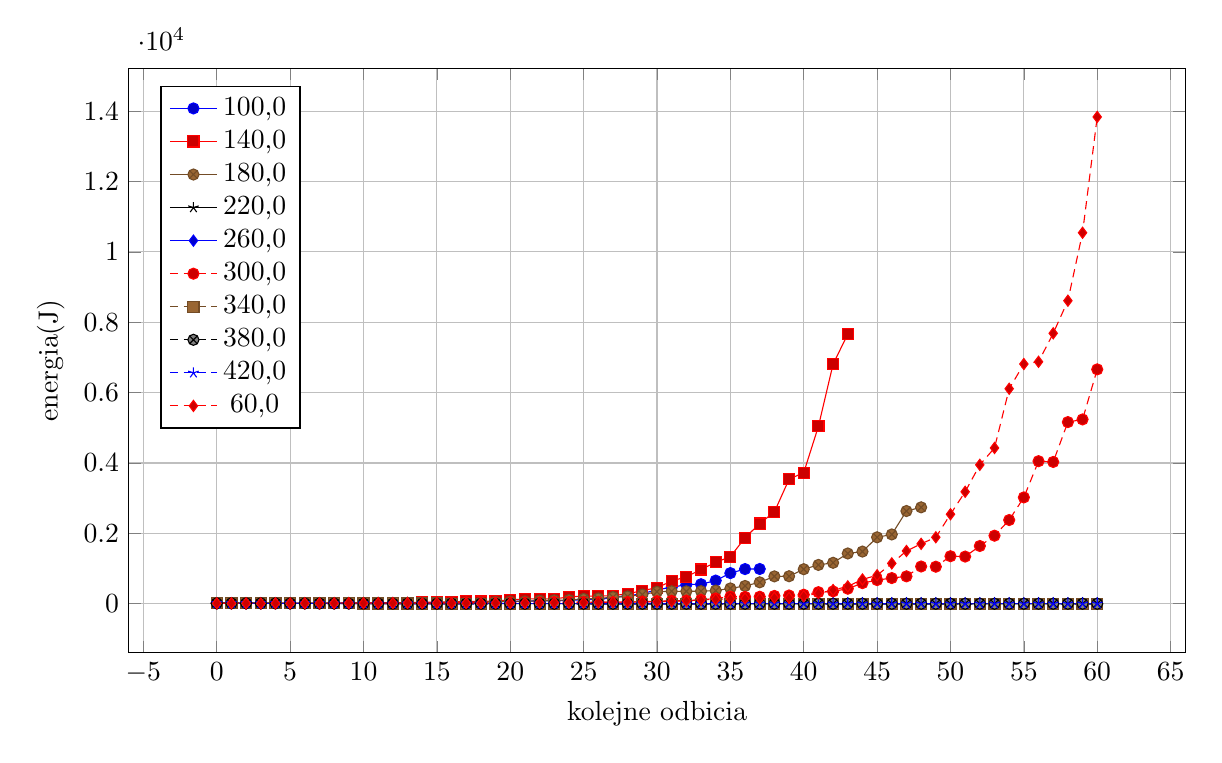
\begin{tikzpicture}
\begin{axis}[
height=9cm,
width=15cm,
grid=major,
xlabel=kolejne odbicia,
ylabel=energia(J),
legend style = { legend pos = north west }
]
\addplot coordinates {(0, 12.5 ) (1, 12.49999 ) (2, 12.499824 ) (3, 12.498202 ) (4, 12.481768 ) (5, 12.316477 ) (6, 15.795458 ) (7, 15.392218 ) (8, 15.434127 ) (9, 15.410436 ) (10, 15.239715 ) (11, 20.11805 ) (12, 19.633654 ) (13, 20.956968 ) (14, 22.878029 ) (15, 31.070366 ) (16, 38.64726 ) (17, 39.382668 ) (18, 52.701916 ) (19, 52.103355 ) (20, 63.929455 ) (21, 74.69516 ) (22, 79.91147 ) (23, 81.80447 ) (24, 95.30267 ) (25, 116.33796 ) (26, 122.753006 ) (27, 171.626 ) (28, 225.77719 ) (29, 282.66235 ) (30, 402.16544 ) (31, 462.3927 ) (32, 545.8912 ) (33, 554.0528 ) (34, 657.7108 ) (35, 869.9793 ) (36, 985.12476 ) (37, 987.26605 ) };
\addlegendentry{100,0}
\addplot coordinates {(0, 12.5 ) (1, 12.499967 ) (2, 12.499719 ) (3, 12.496181 ) (4, 12.446304 ) (5, 11.755087 ) (6, 11.572497 ) (7, 12.945028 ) (8, 12.642736 ) (9, 15.052362 ) (10, 13.829583 ) (11, 17.761051 ) (12, 22.982285 ) (13, 30.615692 ) (14, 38.457775 ) (15, 47.436565 ) (16, 58.842197 ) (17, 64.2831 ) (18, 62.14132 ) (19, 80.48335 ) (20, 108.55065 ) (21, 133.80923 ) (22, 139.68195 ) (23, 137.094 ) (24, 191.534 ) (25, 219.08894 ) (26, 215.14224 ) (27, 230.26402 ) (28, 281.01144 ) (29, 373.2563 ) (30, 456.31274 ) (31, 643.2415 ) (32, 765.12286 ) (33, 972.59406 ) (34, 1176.4192 ) (35, 1337.1683 ) (36, 1875.6881 ) (37, 2279.3777 ) (38, 2609.1792 ) (39, 3538.376 ) (40, 3725.553 ) (41, 5041.8345 ) (42, 6811.656 ) (43, 7661.2676 ) };
\addlegendentry{140,0}
\addplot coordinates {(0, 12.5 ) (1, 12.500086 ) (2, 12.501545 ) (3, 12.527953 ) (4, 13.00956 ) (5, 16.828875 ) (6, 15.706829 ) (7, 15.004946 ) (8, 14.830004 ) (9, 17.307192 ) (10, 18.304008 ) (11, 22.046404 ) (12, 20.210443 ) (13, 23.944548 ) (14, 29.67809 ) (15, 30.661171 ) (16, 36.484932 ) (17, 35.100254 ) (18, 40.778275 ) (19, 55.056026 ) (20, 64.672775 ) (21, 65.86728 ) (22, 87.03496 ) (23, 95.66851 ) (24, 104.94852 ) (25, 137.02641 ) (26, 147.80406 ) (27, 188.14395 ) (28, 206.13316 ) (29, 259.87714 ) (30, 339.46973 ) (31, 353.81726 ) (32, 351.1574 ) (33, 356.59348 ) (34, 372.64868 ) (35, 435.89276 ) (36, 505.09164 ) (37, 608.1733 ) (38, 777.6239 ) (39, 781.0758 ) (40, 980.99603 ) (41, 1103.1704 ) (42, 1163.442 ) (43, 1428.3059 ) (44, 1482.0144 ) (45, 1887.713 ) (46, 1969.0378 ) (47, 2634.8774 ) (48, 2739.9836 ) };
\addlegendentry{180,0}
\addplot coordinates {(0, 12.5 ) (1, 12.499971 ) (2, 12.498856 ) (3, 12.470235 ) (4, 11.736132 ) (5, 11.689475 ) (6, 9.801909 ) (7, 8.49379 ) (8, 7.395703 ) (9, 8.466985 ) (10, 7.53862 ) (11, 7.24089 ) (12, 8.123841 ) (13, 6.475091 ) (14, 6.414579 ) (15, 5.3106594 ) (16, 5.4164762 ) (17, 4.3162026 ) (18, 3.296064 ) (19, 2.739808 ) (20, 2.5333169 ) (21, 1.987436 ) (22, 1.6969215 ) (23, 1.4240198 ) (24, 1.0527757 ) (25, 0.6289513 ) (26, 0.38676772 ) (27, 0.17112246 ) (28, 0.0 ) (29, 0.0 ) (30, 0.0 ) (31, 0.0 ) (32, 0.0 ) (33, 0.0 ) (34, 0.0 ) (35, 0.0 ) (36, 0.0 ) (37, 0.0 ) (38, 0.0 ) (39, 0.0 ) (40, 0.0 ) (41, 0.0 ) (42, 0.0 ) (43, 0.0 ) (44, 0.0 ) (45, 0.0 ) (46, 0.0 ) (47, 0.0 ) (48, 0.0 ) (49, 0.0 ) (50, 0.0 ) (51, 0.0 ) (52, 0.0 ) (53, 0.0 ) (54, 0.0 ) (55, 0.0 ) (56, 0.0 ) (57, 0.0 ) (58, 0.0 ) (59, 0.0 ) (60, 0.0 ) };
\addlegendentry{220,0}
\addplot coordinates {(0, 12.5 ) (1, 12.5 ) (2, 12.5 ) (3, 12.5 ) (4, 12.5 ) (5, 12.5 ) (6, 12.5 ) (7, 12.5 ) (8, 12.5 ) (9, 12.5 ) (10, 12.5 ) (11, 12.5 ) (12, 12.5 ) (13, 12.5 ) (14, 12.5 ) (15, 12.5 ) (16, 12.5 ) (17, 12.5 ) (18, 12.5 ) (19, 12.5 ) (20, 12.5 ) (21, 12.5 ) (22, 12.5 ) (23, 12.5 ) (24, 12.5 ) (25, 12.5 ) (26, 12.5 ) (27, 12.5 ) (28, 12.5 ) (29, 12.5 ) (30, 12.5 ) (31, 12.5 ) (32, 12.5 ) (33, 12.5 ) (34, 12.5 ) (35, 12.5 ) (36, 12.5 ) (37, 12.5 ) (38, 12.5 ) (39, 12.5 ) (40, 12.5 ) (41, 12.5 ) (42, 12.5 ) (43, 12.5 ) (44, 12.5 ) (45, 12.5 ) (46, 12.5 ) (47, 12.5 ) (48, 12.5 ) (49, 12.5 ) (50, 12.5 ) (51, 12.5 ) (52, 12.5 ) (53, 12.5 ) (54, 12.5 ) (55, 12.5 ) (56, 12.5 ) (57, 12.5 ) (58, 12.5 ) (59, 12.5 ) (60, 12.5 ) };
\addlegendentry{260,0}
\addplot coordinates {(0, 12.499857 ) (1, 12.495675 ) (2, 12.370698 ) (3, 13.60359 ) (4, 13.500814 ) (5, 11.857204 ) (6, 13.439519 ) (7, 13.624933 ) (8, 15.260229 ) (9, 15.055403 ) (10, 17.272354 ) (11, 17.70488 ) (12, 17.010616 ) (13, 20.71158 ) (14, 20.718487 ) (15, 24.961153 ) (16, 29.187761 ) (17, 34.821487 ) (18, 30.847595 ) (19, 28.75227 ) (20, 32.012222 ) (21, 32.095547 ) (22, 37.203342 ) (23, 48.29855 ) (24, 49.83079 ) (25, 45.833984 ) (26, 43.64385 ) (27, 41.03238 ) (28, 47.254562 ) (29, 57.411808 ) (30, 70.60043 ) (31, 82.11667 ) (32, 85.857285 ) (33, 109.84031 ) (34, 148.7622 ) (35, 201.23523 ) (36, 194.39172 ) (37, 198.31165 ) (38, 222.07056 ) (39, 234.42426 ) (40, 256.3978 ) (41, 328.6761 ) (42, 350.54938 ) (43, 426.6949 ) (44, 585.76324 ) (45, 671.96454 ) (46, 729.54614 ) (47, 778.2264 ) (48, 1058.2607 ) (49, 1052.0831 ) (50, 1350.322 ) (51, 1340.2926 ) (52, 1641.1189 ) (53, 1933.7147 ) (54, 2379.2126 ) (55, 3022.0554 ) (56, 4051.6084 ) (57, 4029.8694 ) (58, 5162.7783 ) (59, 5238.7476 ) (60, 6661.5063 ) };
\addlegendentry{300,0}
\addplot coordinates {(0, 12.5 ) (1, 12.500324 ) (2, 12.510459 ) (3, 12.8578205 ) (4, 14.523903 ) (5, 14.485657 ) (6, 14.996248 ) (7, 13.288555 ) (8, 10.443586 ) (9, 9.050881 ) (10, 7.6211677 ) (11, 6.8238263 ) (12, 7.3748183 ) (13, 5.9362407 ) (14, 5.6662164 ) (15, 4.837941 ) (16, 3.3367136 ) (17, 2.1178775 ) (18, 1.5461127 ) (19, 0.7480319 ) (20, 0.3167913 ) (21, 0.0 ) (22, 0.0 ) (23, 0.0 ) (24, 0.0 ) (25, 0.0 ) (26, 0.0 ) (27, 0.0 ) (28, 0.0 ) (29, 0.0 ) (30, 0.0 ) (31, 0.0 ) (32, 0.0 ) (33, 0.0 ) (34, 0.0 ) (35, 0.0 ) (36, 0.0 ) (37, 0.0 ) (38, 0.0 ) (39, 0.0 ) (40, 0.0 ) (41, 0.0 ) (42, 0.0 ) (43, 0.0 ) (44, 0.0 ) (45, 0.0 ) (46, 0.0 ) (47, 0.0 ) (48, 0.0 ) (49, 0.0 ) (50, 0.0 ) (51, 0.0 ) (52, 0.0 ) (53, 0.0 ) (54, 0.0 ) (55, 0.0 ) (56, 0.0 ) (57, 0.0 ) (58, 0.0 ) (59, 0.0 ) (60, 0.0 ) };
\addlegendentry{340,0}
\addplot coordinates {(0, 12.499819 ) (1, 12.493163 ) (2, 12.240214 ) (3, 12.464691 ) (4, 10.947274 ) (5, 8.125346 ) (6, 8.594709 ) (7, 7.6774254 ) (8, 7.2305574 ) (9, 5.434474 ) (10, 4.619633 ) (11, 4.406925 ) (12, 3.0008664 ) (13, 2.1981838 ) (14, 1.2431407 ) (15, 0.49624294 ) (16, 0.1068056 ) (17, 0.0 ) (18, 0.0 ) (19, 0.0 ) (20, 0.0 ) (21, 0.0 ) (22, 0.0 ) (23, 0.0 ) (24, 0.0 ) (25, 0.0 ) (26, 0.0 ) (27, 0.0 ) (28, 0.0 ) (29, 0.0 ) (30, 0.0 ) (31, 0.0 ) (32, 0.0 ) (33, 0.0 ) (34, 0.0 ) (35, 0.0 ) (36, 0.0 ) (37, 0.0 ) (38, 0.0 ) (39, 0.0 ) (40, 0.0 ) (41, 0.0 ) (42, 0.0 ) (43, 0.0 ) (44, 0.0 ) (45, 0.0 ) (46, 0.0 ) (47, 0.0 ) (48, 0.0 ) (49, 0.0 ) (50, 0.0 ) (51, 0.0 ) (52, 0.0 ) (53, 0.0 ) (54, 0.0 ) (55, 0.0 ) (56, 0.0 ) (57, 0.0 ) (58, 0.0 ) (59, 0.0 ) (60, 0.0 ) };
\addlegendentry{380,0}
\addplot coordinates {(0, 12.499952 ) (1, 12.496996 ) (2, 12.374047 ) (3, 12.170701 ) (4, 13.262201 ) (5, 12.808096 ) (6, 10.978055 ) (7, 8.181279 ) (8, 5.8180957 ) (9, 3.9461956 ) (10, 2.943127 ) (11, 1.8900867 ) (12, 0.7694603 ) (13, 0.18109135 ) (14, 0.0 ) (15, 0.0 ) (16, 0.0 ) (17, 0.0 ) (18, 0.0 ) (19, 0.0 ) (20, 0.0 ) (21, 0.0 ) (22, 0.0 ) (23, 0.0 ) (24, 0.0 ) (25, 0.0 ) (26, 0.0 ) (27, 0.0 ) (28, 0.0 ) (29, 0.0 ) (30, 0.0 ) (31, 0.0 ) (32, 0.0 ) (33, 0.0 ) (34, 0.0 ) (35, 0.0 ) (36, 0.0 ) (37, 0.0 ) (38, 0.0 ) (39, 0.0 ) (40, 0.0 ) (41, 0.0 ) (42, 0.0 ) (43, 0.0 ) (44, 0.0 ) (45, 0.0 ) (46, 0.0 ) (47, 0.0 ) (48, 0.0 ) (49, 0.0 ) (50, 0.0 ) (51, 0.0 ) (52, 0.0 ) (53, 0.0 ) (54, 0.0 ) (55, 0.0 ) (56, 0.0 ) (57, 0.0 ) (58, 0.0 ) (59, 0.0 ) (60, 0.0 ) };
\addlegendentry{420,0}
\addplot coordinates {(0, 12.499843 ) (1, 12.496562 ) (2, 12.424397 ) (3, 10.886884 ) (4, 13.046445 ) (5, 12.5084505 ) (6, 13.237075 ) (7, 13.062155 ) (8, 15.385118 ) (9, 18.319933 ) (10, 16.32064 ) (11, 16.517368 ) (12, 18.403559 ) (13, 19.003183 ) (14, 16.835337 ) (15, 20.577127 ) (16, 18.870127 ) (17, 16.623774 ) (18, 16.237015 ) (19, 19.964533 ) (20, 23.88816 ) (21, 23.885115 ) (22, 28.107521 ) (23, 31.02433 ) (24, 30.24109 ) (25, 34.535496 ) (26, 41.797955 ) (27, 48.575058 ) (28, 45.46424 ) (29, 54.809666 ) (30, 55.302063 ) (31, 71.383934 ) (32, 82.345955 ) (33, 110.72234 ) (34, 126.86653 ) (35, 134.21808 ) (36, 150.34375 ) (37, 150.72348 ) (38, 170.36002 ) (39, 164.05544 ) (40, 215.57913 ) (41, 297.53812 ) (42, 387.99023 ) (43, 492.70255 ) (44, 689.79504 ) (45, 809.95984 ) (46, 1146.606 ) (47, 1499.0939 ) (48, 1702.364 ) (49, 1888.4081 ) (50, 2543.7822 ) (51, 3181.9275 ) (52, 3947.7117 ) (53, 4427.7295 ) (54, 6110.7974 ) (55, 6813.356 ) (56, 6875.91 ) (57, 7686.6367 ) (58, 8613.109 ) (59, 10545.106 ) (60, 13836.22 ) };
\addlegendentry{60,0}
\end{axis}
\end{tikzpicture}


Dla lepszej czytelności wykresu poniżej znajdują się wartości energii dla
pierwszych 15 odbić:

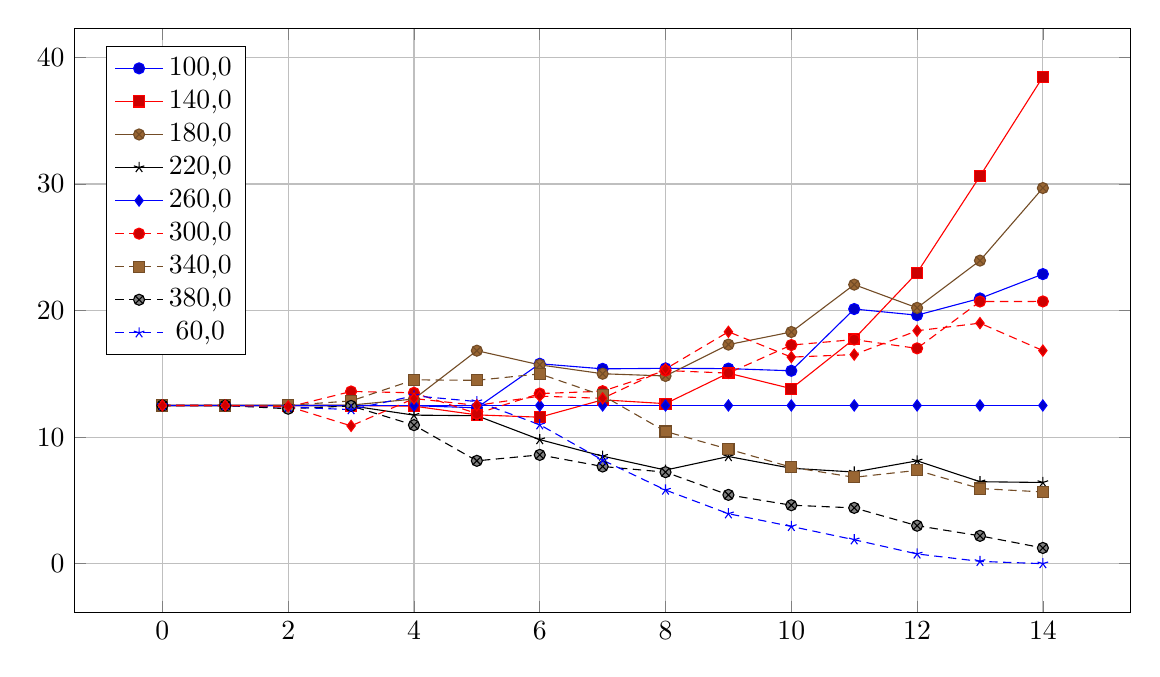
\begin{tikzpicture}
\begin{axis}[
height=9cm,
width=15cm,
grid=major,
legend style = { legend pos = north west }
]
\addplot coordinates {(0, 12.5 ) (1, 12.49999 ) (2, 12.499824 ) (3, 12.498202 ) (4, 12.481768 ) (5, 12.316477 ) (6, 15.795458 ) (7, 15.392218 ) (8, 15.434127 ) (9, 15.410436 ) (10, 15.239715 ) (11, 20.11805 ) (12, 19.633654 ) (13, 20.956968 ) (14, 22.878029 )};
\addlegendentry{100,0}
\addplot coordinates {(0, 12.5 ) (1, 12.499967 ) (2, 12.499719 ) (3, 12.496181 ) (4, 12.446304 ) (5, 11.755087 ) (6, 11.572497 ) (7, 12.945028 ) (8, 12.642736 ) (9, 15.052362 ) (10, 13.829583 ) (11, 17.761051 ) (12, 22.982285 ) (13, 30.615692 ) (14, 38.457775 )};
\addlegendentry{140,0}
\addplot coordinates {(0, 12.5 ) (1, 12.500086 ) (2, 12.501545 ) (3, 12.527953 ) (4, 13.00956 ) (5, 16.828875 ) (6, 15.706829 ) (7, 15.004946 ) (8, 14.830004 ) (9, 17.307192 ) (10, 18.304008 ) (11, 22.046404 ) (12, 20.210443 ) (13, 23.944548 ) (14, 29.67809 )};
\addlegendentry{180,0}
\addplot coordinates {(0, 12.5 ) (1, 12.499971 ) (2, 12.498856 ) (3, 12.470235 ) (4, 11.736132 ) (5, 11.689475 ) (6, 9.801909 ) (7, 8.49379 ) (8, 7.395703 ) (9, 8.466985 ) (10, 7.53862 ) (11, 7.24089 ) (12, 8.123841 ) (13, 6.475091 ) (14, 6.414579 )};
\addlegendentry{220,0}
\addplot coordinates {(0, 12.5 ) (1, 12.5 ) (2, 12.5 ) (3, 12.5 ) (4, 12.5 ) (5, 12.5 ) (6, 12.5 ) (7, 12.5 ) (8, 12.5 ) (9, 12.5 ) (10, 12.5 ) (11, 12.5 ) (12, 12.5 ) (13, 12.5 ) (14, 12.5 )};
\addlegendentry{260,0}
\addplot coordinates {(0, 12.499857 ) (1, 12.495675 ) (2, 12.370698 ) (3, 13.60359 ) (4, 13.500814 ) (5, 11.857204 ) (6, 13.439519 ) (7, 13.624933 ) (8, 15.260229 ) (9, 15.055403 ) (10, 17.272354 ) (11, 17.70488 ) (12, 17.010616 ) (13, 20.71158 ) (14, 20.718487 )};
\addlegendentry{300,0}
\addplot coordinates {(0, 12.5 ) (1, 12.500324 ) (2, 12.510459 ) (3, 12.8578205 ) (4, 14.523903 ) (5, 14.485657 ) (6, 14.996248 ) (7, 13.288555 ) (8, 10.443586 ) (9, 9.050881 ) (10, 7.6211677 ) (11, 6.8238263 ) (12, 7.3748183 ) (13, 5.9362407 ) (14, 5.6662164 )};
\addlegendentry{340,0}
\addplot coordinates {(0, 12.499819 ) (1, 12.493163 ) (2, 12.240214 ) (3, 12.464691 ) (4, 10.947274 ) (5, 8.125346 ) (6, 8.594709 ) (7, 7.6774254 ) (8, 7.2305574 ) (9, 5.434474 ) (10, 4.619633 ) (11, 4.406925 ) (12, 3.0008664 ) (13, 2.1981838 ) (14, 1.2431407 )};
\addlegendentry{380,0}
\addplot coordinates {(0, 12.499952 ) (1, 12.496996 ) (2, 12.374047 ) (3, 12.170701 ) (4, 13.262201 ) (5, 12.808096 ) (6, 10.978055 ) (7, 8.181279 ) (8, 5.8180957 ) (9, 3.9461956 ) (10, 2.943127 ) (11, 1.8900867 ) (12, 0.7694603 ) (13, 0.18109135 ) (14, 0.0 )};
\addlegendentry{60,0}
\addplot coordinates {(0, 12.499843 ) (1, 12.496562 ) (2, 12.424397 ) (3, 10.886884 ) (4, 13.046445 ) (5, 12.5084505 ) (6, 13.237075 ) (7, 13.062155 ) (8, 15.385118 ) (9, 18.319933 ) (10, 16.32064 ) (11, 16.517368 ) (12, 18.403559 ) (13, 19.003183 ) (14, 16.835337 )};
\end{axis}
\end{tikzpicture}


Z wyników można odczytać, że przy długości podkroku $ \frac{1}{260} $ sekundy
zasada zachowanaia energii zostaje spełniona. Okazuje się również, że wartość
tego parametru musi być odpowiednio dobrana (przy innych widoczne są
niedobory/nadmiary energii). Aby sprawdzić czy jest ona uniwersalna, kolejny
test zostanie przeprowadzony dla wartości prędkości 10$\frac{m}{s}$.

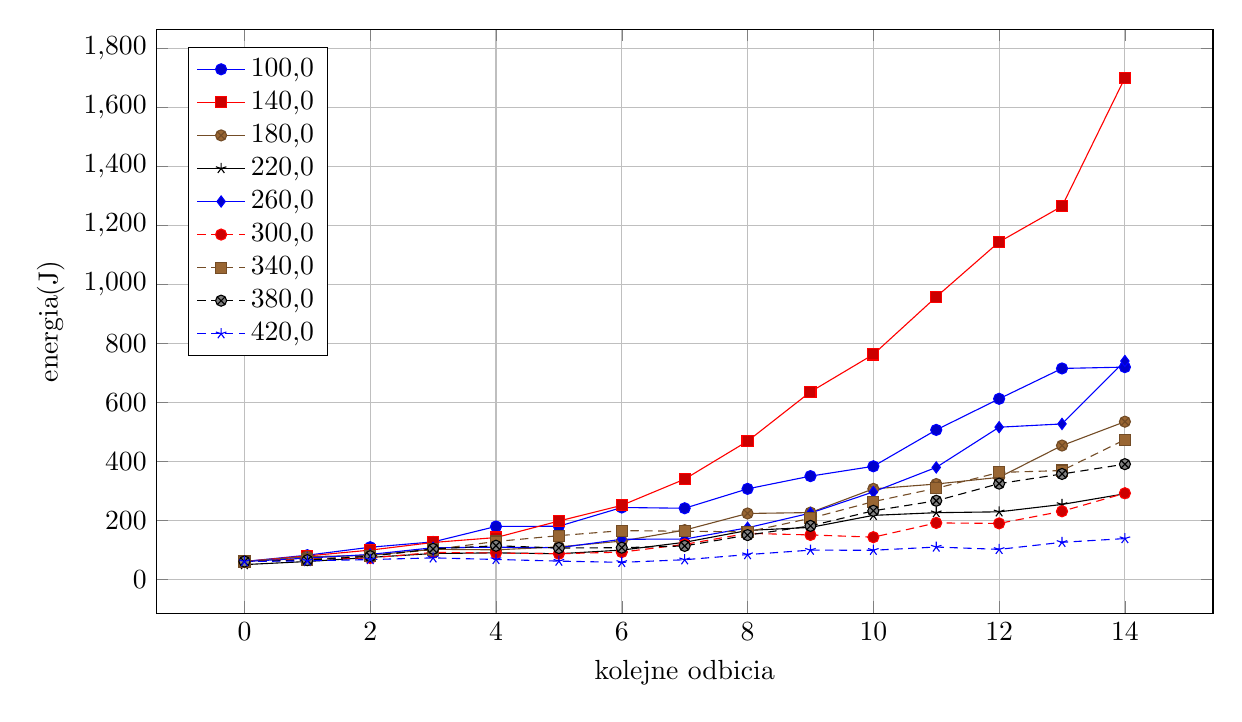
\begin{tikzpicture}
\begin{axis}[
height=9cm,
width=15cm,
grid=major,
xlabel=kolejne odbicia,
ylabel=energia(J),
legend style = { legend pos = north west }
]
\addplot coordinates {(0, 60.500023 ) (1, 81.92009 ) (2, 108.92922 ) (3, 126.9798 ) (4, 179.415 ) (5, 180.04378 ) (6, 243.66458 ) (7, 241.06052 ) (8, 306.84937 ) (9, 350.00568 ) (10, 383.3237 ) (11, 506.71848 ) (12, 612.16895 ) (13, 715.15283 ) (14, 719.6333 )};
\addlegendentry{100,0}
\addplot coordinates {(0, 60.5 ) (1, 79.38007 ) (2, 99.12363 ) (3, 125.07543 ) (4, 141.69774 ) (5, 197.75262 ) (6, 251.01779 ) (7, 339.7764 ) (8, 468.51224 ) (9, 635.6914 ) (10, 762.6489 ) (11, 957.757 ) (12, 1144.0896 ) (13, 1265.168 ) (14, 1700.5425 )};
\addlegendentry{140,0}
\addplot coordinates {(0, 60.50015 ) (1, 76.881676 ) (2, 81.42158 ) (3, 101.95011 ) (4, 100.09618 ) (5, 110.0021 ) (6, 129.7769 ) (7, 166.9779 ) (8, 223.40483 ) (9, 226.44267 ) (10, 306.8936 ) (11, 323.2172 ) (12, 345.97656 ) (13, 453.7002 ) (14, 534.60846 )};
\addlegendentry{180,0}
\addplot coordinates {(0, 50.0 ) (1, 60.499874 ) (2, 74.41864 ) (3, 87.634735 ) (4, 89.8731 ) (5, 86.80204 ) (6, 99.18527 ) (7, 125.629486 ) (8, 165.85115 ) (9, 176.15439 ) (10, 216.987 ) (11, 226.05557 ) (12, 228.96167 ) (13, 253.99066 ) (14, 290.1967 )};
\addlegendentry{220,0}
\addplot coordinates {(0, 60.500317 ) (1, 72.004326 ) (2, 84.55166 ) (3, 107.17797 ) (4, 109.10671 ) (5, 107.09075 ) (6, 135.90282 ) (7, 136.57355 ) (8, 174.91646 ) (9, 224.60782 ) (10, 296.45978 ) (11, 379.62122 ) (12, 515.9012 ) (13, 527.0016 ) (14, 740.21735 )};
\addlegendentry{260,0}
\addplot coordinates {(0, 60.500065 ) (1, 69.62055 ) (2, 72.48745 ) (3, 91.272835 ) (4, 89.28663 ) (5, 86.829384 ) (6, 92.37034 ) (7, 118.69746 ) (8, 156.08209 ) (9, 150.57904 ) (10, 143.00375 ) (11, 191.29128 ) (12, 189.68774 ) (13, 230.79619 ) (14, 292.0326 )};
\addlegendentry{300,0}
\addplot coordinates {(0, 60.500546 ) (1, 67.28903 ) (2, 80.538994 ) (3, 100.922035 ) (4, 128.30896 ) (5, 148.18803 ) (6, 165.16585 ) (7, 163.09677 ) (8, 161.04451 ) (9, 207.07037 ) (10, 263.59717 ) (11, 308.80777 ) (12, 362.447 ) (13, 368.95673 ) (14, 473.61365 )};
\addlegendentry{340,0}
\addplot coordinates {(0, 60.50036 ) (1, 64.98713 ) (2, 78.50689 ) (3, 103.256546 ) (4, 113.94582 ) (5, 106.305664 ) (6, 107.335 ) (7, 113.28537 ) (8, 150.0018 ) (9, 181.31984 ) (10, 232.42296 ) (11, 266.4738 ) (12, 324.6097 ) (13, 357.30115 ) (14, 390.61658 )};
\addlegendentry{380,0}
\addplot coordinates {(0, 60.50084 ) (1, 62.73556 ) (2, 67.12027 ) (3, 72.84919 ) (4, 67.44308 ) (5, 61.86573 ) (6, 57.622555 ) (7, 66.51577 ) (8, 83.97656 ) (9, 99.01908 ) (10, 98.68342 ) (11, 109.573204 ) (12, 101.67075 ) (13, 125.58686 ) (14, 138.26483 )};
\addlegendentry{420,0}
\end{axis}
\end{tikzpicture}


Jak widać odpowiednia wartość parametru \emph{fixedTimeStep} jest uzależniona od
wartości prędkości. Poprawne zasymulowanie doświadczenia w którym ważną rolę
odgrywają odbicia sprężyste przy użyciu silnika Bullet jest więc bardzo trudne.

\subsubsection{Odbicie sprężyste wielu ciał}\label{sec:odbicieWieluCial}

W poprzednim doświadczeniu został zbadany przypadek dla jednego ciała i dla
wartości kroku $ \frac{1}{260} $s i prędkości 5$ \frac{m}{s} $ energia
kinetyczna pozostaje stała. Jak wyglądać będzie zależność energii kinetycznej od
czasu w tych samych warunkach jeśli w symulacji będzie uczestniczyć wiele ciał?
Przy pomocy poniższej sceny sprawdzone zostanie jaki wpływ ma parametr
\emph{fixedTimeStep} na łączną energię poruszających się ciał.

\begin{center}
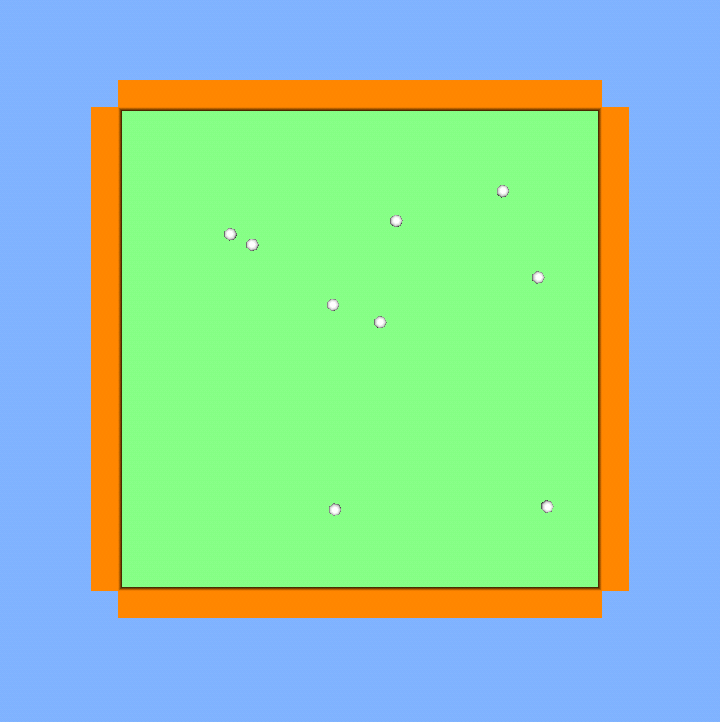
\includegraphics[scale = 0.5]{./img/shot_2.png}
\end{center}

\lstinputlisting[language=Java,
  label=lis:ClosedSnookerScene,caption=scena
  testująca przypadek z wieloma ciałami]{./listings/ClosedSnookerScene3.java}
  
Na obszarze otoczonym ściankami (ln. 44-50) zostaje umieszczonych dziewięć (ln.
60-66) idealnie sprężystych (ln. 69) kulek. Kulki rozprzestrzeniają się w
losowych kierunkach z prędkością 5$ \frac{m}{s} $ (ln. 64). Wartość energii
kinetycznej całego układu jest rejestrowana co 20 klatek (ln. 22, 105-111).
Każdy test trwa 20*100 klatek (ln. 22, 24, 94), w każdym z nich wartość
parametru \emph{ftsFactor} jest zwiększana (ln. 101).\\
Poniżej przedstawiono wykres zależności całkowitej energii układu od
czasu (klatek animacji) dla różnych wartości \emph{ftsFactor}, a tym samym
długości podkroku symulacji. Dla większej dokładności wykonane zostało dziesięć
takich testów i wyciągnięta zostałą z nich średnia wartość energii.

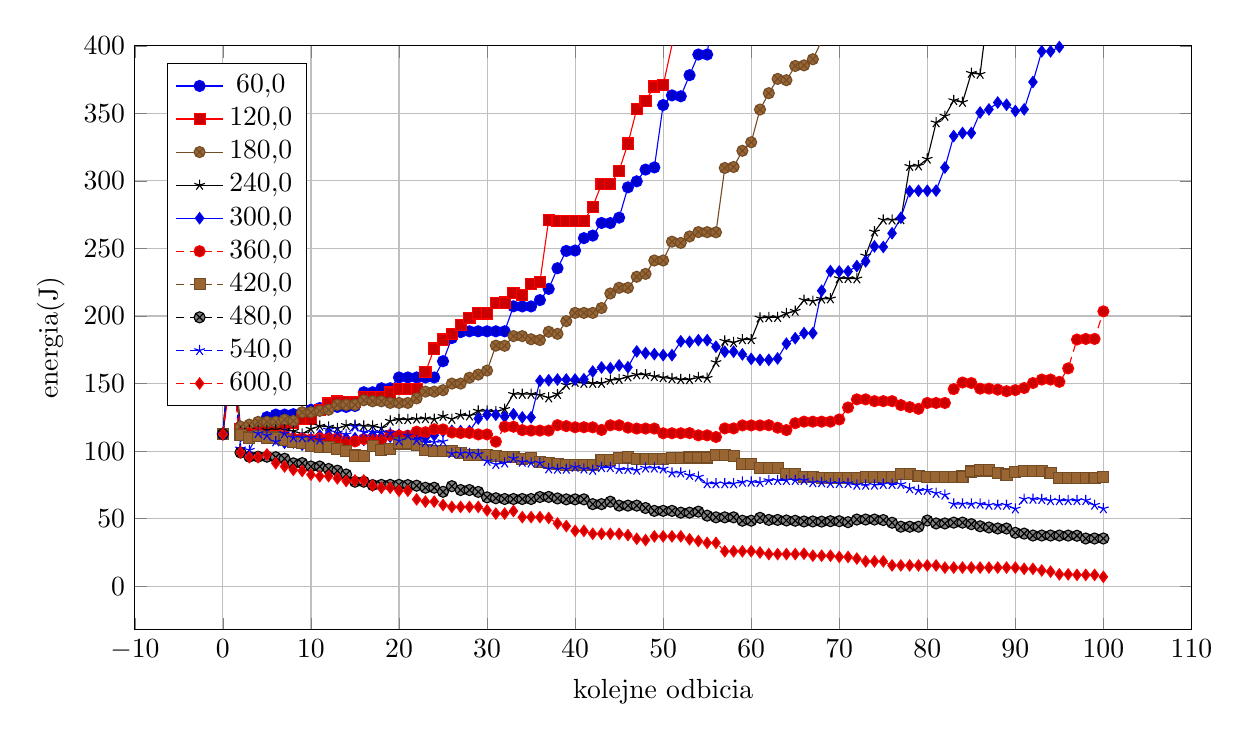
\begin{tikzpicture}
\begin{axis}[
height=9cm,
width=15cm,
grid=major,
ymax=400,
xlabel=kolejne odbicia,
ylabel=energia(J),
legend style = { legend pos = north west }
]
\addplot coordinates {(0, 113.00001 ) (1, 184.5 ) (2, 112.50238 ) (3, 117.51947 ) (4, 117.94633 ) (5, 125.13693 ) (6, 127.014 ) (7, 127.01402 ) (8, 127.32728 ) (9, 127.327324 ) (10, 130.59416 ) (11, 131.85373 ) (12, 131.71252 ) (13, 132.71825 ) (14, 132.71829 ) (15, 133.37012 ) (16, 143.56427 ) (17, 143.56427 ) (18, 146.50638 ) (19, 146.5063 ) (20, 154.51622 ) (21, 154.51622 ) (22, 154.51616 ) (23, 154.51613 ) (24, 154.51616 ) (25, 166.53984 ) (26, 183.64267 ) (27, 188.08847 ) (28, 188.67494 ) (29, 188.67488 ) (30, 188.67485 ) (31, 188.67485 ) (32, 188.67485 ) (33, 207.16179 ) (34, 207.09554 ) (35, 207.09557 ) (36, 211.77588 ) (37, 220.0541 ) (38, 235.3764 ) (39, 248.17258 ) (40, 248.44806 ) (41, 257.6311 ) (42, 259.50778 ) (43, 268.88147 ) (44, 268.7858 ) (45, 272.79675 ) (46, 295.2298 ) (47, 299.69308 ) (48, 308.36163 ) (49, 309.97687 ) (50, 356.14392 ) (51, 363.29996 ) (52, 362.6423 ) (53, 378.25986 ) (54, 393.5498 ) (55, 393.54974 ) (56, 445.67075 ) (57, 456.77032 ) (58, 463.24442 ) (59, 502.17465 ) (60, 522.92065 ) (61, 563.43066 ) (62, 597.61694 ) (63, 597.40765 ) (64, 629.5412 ) (65, 630.4578 ) (66, 701.16095 ) (67, 701.161 ) (68, 735.1671 ) (69, 751.31036 ) (70, 828.1006 ) (71, 866.8466 ) (72, 881.93823 ) (73, 902.79346 ) (74, 930.66785 ) (75, 962.0779 ) (76, 992.9918 ) (77, 1084.1486 ) (78, 1084.148 ) (79, 1253.6515 ) (80, 1276.0906 ) (81, 1276.093 ) (82, 1290.94 ) (83, 1394.8301 ) (84, 1398.7712 ) (85, 1550.5096 ) (86, 1563.2556 ) (87, 1565.5009 ) (88, 1621.0059 ) (89, 1711.5502 ) (90, 1885.5609 ) (91, 1951.7416 ) (92, 2078.3628 ) (93, 2148.7722 ) (94, 2146.4148 ) (95, 2485.3906 ) (96, 2533.255 ) (97, 2682.5635 ) (98, 2665.1897 ) (99, 2670.038 ) (100, 2736.718 ) };
\addlegendentry{60,0}
\addplot coordinates {(0, 112.5487 ) (1, 162.54868 ) (2, 116.17382 ) (3, 117.36174 ) (4, 117.62299 ) (5, 118.34479 ) (6, 119.519165 ) (7, 121.04038 ) (8, 121.04039 ) (9, 123.55827 ) (10, 123.55829 ) (11, 130.30643 ) (12, 135.21194 ) (13, 136.7269 ) (14, 136.13672 ) (15, 136.13672 ) (16, 139.88422 ) (17, 140.28423 ) (18, 140.25903 ) (19, 143.35568 ) (20, 145.99844 ) (21, 145.99844 ) (22, 146.17267 ) (23, 158.29214 ) (24, 175.91222 ) (25, 182.5776 ) (26, 186.8992 ) (27, 193.5506 ) (28, 198.62366 ) (29, 201.90523 ) (30, 201.9052 ) (31, 209.42941 ) (32, 209.94998 ) (33, 216.7919 ) (34, 215.64314 ) (35, 223.43353 ) (36, 225.07977 ) (37, 271.35974 ) (38, 270.23114 ) (39, 270.23114 ) (40, 270.23117 ) (41, 270.23117 ) (42, 280.8301 ) (43, 297.54373 ) (44, 297.5437 ) (45, 307.57492 ) (46, 327.62485 ) (47, 353.1484 ) (48, 359.17917 ) (49, 369.8787 ) (50, 370.70682 ) (51, 400.4697 ) (52, 408.54193 ) (53, 421.25504 ) (54, 419.25403 ) (55, 433.80887 ) (56, 431.20178 ) (57, 431.2018 ) (58, 470.5524 ) (59, 509.1405 ) (60, 508.8591 ) (61, 530.23065 ) (62, 594.97577 ) (63, 601.9276 ) (64, 644.6806 ) (65, 680.63184 ) (66, 685.6931 ) (67, 727.82025 ) (68, 738.59625 ) (69, 822.3908 ) (70, 840.235 ) (71, 892.39264 ) (72, 966.02264 ) (73, 1029.7766 ) (74, 1177.0339 ) (75, 1262.7404 ) (76, 1381.2922 ) (77, 1472.6456 ) (78, 1641.8782 ) (79, 1673.5479 ) (80, 1794.3059 ) (81, 2065.4512 ) (82, 2201.8027 ) (83, 2594.3845 ) (84, 2921.0886 ) (85, 3193.77 ) (86, 3637.8203 ) (87, 3807.1228 ) (88, 4024.0234 ) (89, 4463.9453 ) (90, 4579.5454 ) (91, 4758.0806 ) (92, 4770.904 ) (93, 4998.985 ) (94, 5117.5063 ) (95, 5347.9927 ) (96, 5387.048 ) (97, 5703.8384 ) (98, 5707.41 ) (99, 5808.9434 ) (100, 5832.7886 ) };
\addlegendentry{120,0}
\addplot coordinates {(0, 112.5487 ) (1, 188.60428 ) (2, 118.184494 ) (3, 119.60726 ) (4, 121.6377 ) (5, 121.63768 ) (6, 121.637695 ) (7, 123.22441 ) (8, 122.286575 ) (9, 128.76872 ) (10, 128.76874 ) (11, 129.7832 ) (12, 130.60263 ) (13, 134.22415 ) (14, 134.22418 ) (15, 134.2242 ) (16, 137.60153 ) (17, 136.85336 ) (18, 136.85342 ) (19, 135.64754 ) (20, 135.636 ) (21, 135.63602 ) (22, 139.0139 ) (23, 144.02792 ) (24, 144.02791 ) (25, 145.09256 ) (26, 149.98236 ) (27, 149.98238 ) (28, 154.3206 ) (29, 156.64667 ) (30, 159.60318 ) (31, 178.06842 ) (32, 177.93794 ) (33, 185.09299 ) (34, 185.09296 ) (35, 182.79509 ) (36, 182.19936 ) (37, 188.33134 ) (38, 186.78049 ) (39, 196.2005 ) (40, 202.29337 ) (41, 202.29337 ) (42, 202.29337 ) (43, 205.91023 ) (44, 216.68524 ) (45, 220.88185 ) (46, 220.88182 ) (47, 229.06004 ) (48, 231.17107 ) (49, 241.08759 ) (50, 241.08762 ) (51, 255.03639 ) (52, 254.10823 ) (53, 258.88876 ) (54, 262.12518 ) (55, 262.06775 ) (56, 261.95395 ) (57, 309.56955 ) (58, 310.30145 ) (59, 322.29605 ) (60, 328.59793 ) (61, 352.8263 ) (62, 364.93353 ) (63, 375.49692 ) (64, 374.54904 ) (65, 385.0919 ) (66, 385.51544 ) (67, 390.05713 ) (68, 403.54578 ) (69, 464.8037 ) (70, 467.00052 ) (71, 508.98898 ) (72, 581.1413 ) (73, 589.7731 ) (74, 630.26776 ) (75, 679.18286 ) (76, 714.548 ) (77, 779.14276 ) (78, 826.9036 ) (79, 824.9287 ) (80, 883.88165 ) (81, 948.7148 ) (82, 972.3597 ) (83, 969.7957 ) (84, 1004.6762 ) (85, 1049.0778 ) (86, 1144.6826 ) (87, 1165.9688 ) (88, 1246.2808 ) (89, 1265.343 ) (90, 1667.6694 ) (91, 1705.874 ) (92, 1743.7566 ) (93, 2079.4739 ) (94, 2302.831 ) (95, 2468.1392 ) (96, 2853.6433 ) (97, 3374.0725 ) (98, 3870.7478 ) (99, 4660.6284 ) (100, 4892.7495 ) };
\addlegendentry{180,0}
\addplot coordinates {(0, 112.548706 ) (1, 190.6738 ) (2, 114.2814 ) (3, 115.51178 ) (4, 115.51177 ) (5, 115.4113 ) (6, 115.73576 ) (7, 115.63976 ) (8, 114.79944 ) (9, 112.79549 ) (10, 116.372635 ) (11, 118.60753 ) (12, 117.920044 ) (13, 116.82765 ) (14, 119.135994 ) (15, 119.13599 ) (16, 118.61494 ) (17, 118.61496 ) (18, 117.05508 ) (19, 122.26758 ) (20, 123.48631 ) (21, 123.37481 ) (22, 123.8188 ) (23, 124.11915 ) (24, 123.590866 ) (25, 125.84889 ) (26, 123.68564 ) (27, 126.767654 ) (28, 126.112434 ) (29, 129.70691 ) (30, 129.70694 ) (31, 129.13838 ) (32, 131.03752 ) (33, 142.16762 ) (34, 142.16762 ) (35, 142.1676 ) (36, 141.50601 ) (37, 139.49097 ) (38, 142.04713 ) (39, 148.9127 ) (40, 151.00247 ) (41, 150.2404 ) (42, 150.24039 ) (43, 150.23058 ) (44, 152.47835 ) (45, 153.12498 ) (46, 154.97937 ) (47, 156.58574 ) (48, 156.61487 ) (49, 155.27151 ) (50, 154.42787 ) (51, 153.65968 ) (52, 153.00595 ) (53, 153.00592 ) (54, 154.5303 ) (55, 154.0096 ) (56, 165.67404 ) (57, 181.488 ) (58, 180.4116 ) (59, 182.57956 ) (60, 182.57956 ) (61, 198.56308 ) (62, 198.97745 ) (63, 198.9775 ) (64, 201.87714 ) (65, 203.65779 ) (66, 211.80878 ) (67, 211.04655 ) (68, 212.62047 ) (69, 212.8369 ) (70, 227.84344 ) (71, 227.84346 ) (72, 227.5782 ) (73, 244.611 ) (74, 262.34482 ) (75, 271.105 ) (76, 271.10498 ) (77, 271.38754 ) (78, 310.84894 ) (79, 311.19476 ) (80, 316.19217 ) (81, 343.11267 ) (82, 347.98102 ) (83, 359.56424 ) (84, 358.25607 ) (85, 379.79208 ) (86, 379.02664 ) (87, 431.86423 ) (88, 429.13278 ) (89, 426.39432 ) (90, 427.00986 ) (91, 462.6108 ) (92, 465.4296 ) (93, 474.08966 ) (94, 508.0888 ) (95, 519.06396 ) (96, 579.9953 ) (97, 613.1723 ) (98, 613.17236 ) (99, 621.8402 ) (100, 634.40436 ) };
\addlegendentry{240,0}
\addplot coordinates {(0, 112.547195 ) (1, 190.67209 ) (2, 111.06951 ) (3, 112.28796 ) (4, 111.16186 ) (5, 111.16186 ) (6, 109.40137 ) (7, 106.17088 ) (8, 106.320076 ) (9, 104.748055 ) (10, 104.360214 ) (11, 111.53779 ) (12, 111.53777 ) (13, 109.82862 ) (14, 109.51774 ) (15, 109.51773 ) (16, 108.279724 ) (17, 111.75267 ) (18, 110.69032 ) (19, 110.69034 ) (20, 111.9788 ) (21, 110.16438 ) (22, 110.16439 ) (23, 110.16438 ) (24, 111.754326 ) (25, 114.815544 ) (26, 114.971115 ) (27, 114.757645 ) (28, 114.75763 ) (29, 124.13789 ) (30, 126.959404 ) (31, 126.879616 ) (32, 125.398926 ) (33, 127.250244 ) (34, 124.9888 ) (35, 124.9888 ) (36, 152.04565 ) (37, 152.4454 ) (38, 152.97066 ) (39, 152.97064 ) (40, 152.97064 ) (41, 153.20851 ) (42, 158.88484 ) (43, 161.91447 ) (44, 161.36707 ) (45, 163.44145 ) (46, 162.0746 ) (47, 173.80046 ) (48, 172.51402 ) (49, 171.75667 ) (50, 171.02705 ) (51, 171.02705 ) (52, 181.29167 ) (53, 180.90913 ) (54, 182.10649 ) (55, 182.10648 ) (56, 177.28188 ) (57, 173.5651 ) (58, 173.5651 ) (59, 171.5787 ) (60, 168.24078 ) (61, 167.54675 ) (62, 167.54677 ) (63, 168.57292 ) (64, 179.50291 ) (65, 183.58499 ) (66, 187.2913 ) (67, 187.2913 ) (68, 218.6821 ) (69, 233.19157 ) (70, 233.01662 ) (71, 233.01665 ) (72, 236.91095 ) (73, 240.46814 ) (74, 251.56276 ) (75, 251.0963 ) (76, 261.2442 ) (77, 272.72922 ) (78, 292.33173 ) (79, 292.71902 ) (80, 292.71902 ) (81, 292.79785 ) (82, 309.87097 ) (83, 333.1766 ) (84, 335.4353 ) (85, 335.4353 ) (86, 350.64938 ) (87, 352.90765 ) (88, 358.01102 ) (89, 356.3911 ) (90, 351.6872 ) (91, 352.97046 ) (92, 373.22345 ) (93, 395.9171 ) (94, 395.91718 ) (95, 399.09937 ) (96, 414.08395 ) (97, 441.72617 ) (98, 441.72617 ) (99, 441.4844 ) (100, 459.6118 ) };
\addlegendentry{300,0}
\addplot coordinates {(0, 112.5472 ) (1, 190.67192 ) (2, 112.52281 ) (3, 113.04143 ) (4, 113.04889 ) (5, 110.13812 ) (6, 111.3356 ) (7, 111.22237 ) (8, 109.267334 ) (9, 109.26733 ) (10, 108.60425 ) (11, 109.396385 ) (12, 109.39638 ) (13, 109.47719 ) (14, 107.19468 ) (15, 107.19469 ) (16, 108.88396 ) (17, 108.584335 ) (18, 108.58434 ) (19, 111.940674 ) (20, 111.46748 ) (21, 111.467476 ) (22, 114.364136 ) (23, 113.973694 ) (24, 116.180145 ) (25, 116.0617 ) (26, 113.8283 ) (27, 113.41484 ) (28, 113.41484 ) (29, 112.32866 ) (30, 112.32864 ) (31, 106.99441 ) (32, 118.10378 ) (33, 118.02884 ) (34, 115.50758 ) (35, 115.182434 ) (36, 115.18242 ) (37, 115.18242 ) (38, 119.19738 ) (39, 118.49403 ) (40, 117.65827 ) (41, 117.65827 ) (42, 117.58594 ) (43, 115.6509 ) (44, 119.10109 ) (45, 119.10109 ) (46, 117.37339 ) (47, 116.680756 ) (48, 116.68074 ) (49, 116.68074 ) (50, 113.198395 ) (51, 113.19838 ) (52, 113.198395 ) (53, 113.319 ) (54, 111.67023 ) (55, 111.67023 ) (56, 110.4317 ) (57, 116.81165 ) (58, 116.811646 ) (59, 119.01294 ) (60, 119.012924 ) (61, 119.012924 ) (62, 119.15817 ) (63, 117.34425 ) (64, 115.55844 ) (65, 120.62912 ) (66, 121.80615 ) (67, 121.80615 ) (68, 121.80614 ) (69, 121.80614 ) (70, 123.42439 ) (71, 132.31058 ) (72, 138.28583 ) (73, 138.28583 ) (74, 136.97827 ) (75, 136.97829 ) (76, 136.97827 ) (77, 134.04884 ) (78, 132.5621 ) (79, 131.28508 ) (80, 135.62997 ) (81, 135.63 ) (82, 135.63002 ) (83, 145.90106 ) (84, 150.7592 ) (85, 150.37581 ) (86, 146.23509 ) (87, 146.23508 ) (88, 145.50775 ) (89, 144.33203 ) (90, 145.15024 ) (91, 146.69049 ) (92, 150.39026 ) (93, 152.96289 ) (94, 152.96292 ) (95, 151.26233 ) (96, 161.24045 ) (97, 182.5897 ) (98, 183.02837 ) (99, 183.0284 ) (100, 203.44574 ) };
\addlegendentry{360,0}
\addplot coordinates {(0, 112.547195 ) (1, 194.28415 ) (2, 111.632355 ) (3, 110.049644 ) (4, 111.1286 ) (5, 110.03436 ) (6, 110.03437 ) (7, 108.031906 ) (8, 106.51633 ) (9, 106.32344 ) (10, 103.77039 ) (11, 103.18259 ) (12, 103.182594 ) (13, 101.571594 ) (14, 100.30214 ) (15, 96.72721 ) (16, 96.26642 ) (17, 103.84975 ) (18, 101.07063 ) (19, 101.74451 ) (20, 105.61685 ) (21, 105.61685 ) (22, 104.52336 ) (23, 100.93434 ) (24, 100.056435 ) (25, 100.05644 ) (26, 100.05646 ) (27, 98.4947 ) (28, 97.154335 ) (29, 97.15434 ) (30, 96.84407 ) (31, 96.11688 ) (32, 95.50562 ) (33, 95.50563 ) (34, 93.98993 ) (35, 94.99203 ) (36, 92.06972 ) (37, 91.39548 ) (38, 90.72854 ) (39, 89.425545 ) (40, 89.425545 ) (41, 89.695496 ) (42, 89.6955 ) (43, 93.53689 ) (44, 93.53689 ) (45, 94.87664 ) (46, 95.30166 ) (47, 94.143005 ) (48, 94.143 ) (49, 94.06567 ) (50, 94.06567 ) (51, 94.88156 ) (52, 94.93149 ) (53, 95.27471 ) (54, 95.27473 ) (55, 95.274704 ) (56, 97.36675 ) (57, 97.36675 ) (58, 96.37755 ) (59, 90.1563 ) (60, 90.156296 ) (61, 87.46427 ) (62, 87.46427 ) (63, 87.464264 ) (64, 83.03211 ) (65, 83.03211 ) (66, 80.73435 ) (67, 80.84324 ) (68, 79.86222 ) (69, 79.86221 ) (70, 79.86221 ) (71, 79.86222 ) (72, 79.862206 ) (73, 81.11015 ) (74, 81.110146 ) (75, 80.63219 ) (76, 80.63218 ) (77, 82.77054 ) (78, 82.77053 ) (79, 81.73924 ) (80, 80.85981 ) (81, 80.85981 ) (82, 80.85981 ) (83, 80.91845 ) (84, 81.18379 ) (85, 84.9008 ) (86, 85.69329 ) (87, 85.69328 ) (88, 83.543015 ) (89, 82.62973 ) (90, 84.75518 ) (91, 85.092636 ) (92, 85.09264 ) (93, 85.09265 ) (94, 83.75458 ) (95, 80.29893 ) (96, 80.29891 ) (97, 80.2989 ) (98, 80.29889 ) (99, 80.31526 ) (100, 80.57387 ) };
\addlegendentry{420,0}
\addplot coordinates {(0, 112.547195 ) (1, 175.15817 ) (2, 98.93977 ) (3, 95.85657 ) (4, 95.856575 ) (5, 95.856575 ) (6, 95.44351 ) (7, 94.33797 ) (8, 90.95447 ) (9, 91.09886 ) (10, 88.60189 ) (11, 88.601906 ) (12, 86.76886 ) (13, 85.50454 ) (14, 82.69193 ) (15, 77.35413 ) (16, 77.354126 ) (17, 74.869705 ) (18, 75.003334 ) (19, 75.00334 ) (20, 75.003365 ) (21, 74.83993 ) (22, 74.40373 ) (23, 72.874176 ) (24, 72.87418 ) (25, 69.872955 ) (26, 74.01319 ) (27, 71.189255 ) (28, 71.18925 ) (29, 69.79193 ) (30, 65.76224 ) (31, 65.10614 ) (32, 64.54094 ) (33, 64.54093 ) (34, 64.54093 ) (35, 64.54093 ) (36, 66.009514 ) (37, 66.08585 ) (38, 64.94906 ) (39, 64.2722 ) (40, 64.272194 ) (41, 64.27219 ) (42, 60.75153 ) (43, 60.751526 ) (44, 62.561535 ) (45, 59.64702 ) (46, 59.647022 ) (47, 59.64702 ) (48, 57.86428 ) (49, 55.763058 ) (50, 55.763058 ) (51, 55.76307 ) (52, 54.446625 ) (53, 54.446632 ) (54, 55.189125 ) (55, 52.236897 ) (56, 50.965137 ) (57, 50.965145 ) (58, 50.96514 ) (59, 48.481686 ) (60, 48.481693 ) (61, 50.605694 ) (62, 49.07302 ) (63, 49.07302 ) (64, 48.65398 ) (65, 48.436768 ) (66, 47.924152 ) (67, 47.924156 ) (68, 47.808086 ) (69, 48.124397 ) (70, 48.124393 ) (71, 47.39555 ) (72, 49.33939 ) (73, 49.339397 ) (74, 49.33941 ) (75, 48.96384 ) (76, 46.983574 ) (77, 44.039356 ) (78, 44.039364 ) (79, 44.03937 ) (80, 48.603657 ) (81, 46.445084 ) (82, 46.445087 ) (83, 47.05646 ) (84, 47.056465 ) (85, 45.91166 ) (86, 44.333637 ) (87, 43.47431 ) (88, 42.695396 ) (89, 42.695408 ) (90, 39.532795 ) (91, 38.924805 ) (92, 37.50961 ) (93, 37.50961 ) (94, 37.509605 ) (95, 37.509598 ) (96, 37.455803 ) (97, 37.342373 ) (98, 35.303818 ) (99, 35.303818 ) (100, 35.303818 ) };
\addlegendentry{480,0}
\addplot coordinates {(0, 112.54707 ) (1, 175.80127 ) (2, 101.784225 ) (3, 100.70917 ) (4, 113.12109 ) (5, 111.6284 ) (6, 106.9591 ) (7, 113.01591 ) (8, 109.93198 ) (9, 109.931984 ) (10, 109.931984 ) (11, 108.32823 ) (12, 115.69409 ) (13, 113.66594 ) (14, 112.28542 ) (15, 117.96128 ) (16, 113.95721 ) (17, 113.9572 ) (18, 113.9572 ) (19, 113.425125 ) (20, 107.62096 ) (21, 111.50984 ) (22, 107.91634 ) (23, 106.45322 ) (24, 106.45322 ) (25, 107.07942 ) (26, 98.21594 ) (27, 98.21596 ) (28, 98.21596 ) (29, 97.72102 ) (30, 92.55907 ) (31, 90.24121 ) (32, 91.27984 ) (33, 94.54258 ) (34, 91.889175 ) (35, 91.27588 ) (36, 91.27587 ) (37, 86.91404 ) (38, 86.66528 ) (39, 86.66528 ) (40, 88.11942 ) (41, 86.79778 ) (42, 85.877525 ) (43, 87.890816 ) (44, 87.890816 ) (45, 86.54853 ) (46, 86.54853 ) (47, 85.87684 ) (48, 87.53368 ) (49, 87.533676 ) (50, 86.85544 ) (51, 83.91884 ) (52, 83.91884 ) (53, 82.105865 ) (54, 80.86132 ) (55, 75.93447 ) (56, 75.93448 ) (57, 75.908264 ) (58, 75.90825 ) (59, 77.13561 ) (60, 77.13561 ) (61, 76.82095 ) (62, 78.316536 ) (63, 78.32471 ) (64, 78.324715 ) (65, 78.3247 ) (66, 78.32471 ) (67, 76.73644 ) (68, 76.73644 ) (69, 76.06266 ) (70, 76.062675 ) (71, 76.06269 ) (72, 74.88372 ) (73, 74.88372 ) (74, 74.88373 ) (75, 75.451256 ) (76, 75.45125 ) (77, 75.45124 ) (78, 72.264366 ) (79, 71.027016 ) (80, 71.02701 ) (81, 68.832016 ) (82, 67.54046 ) (83, 60.85746 ) (84, 60.85744 ) (85, 60.85743 ) (86, 60.85741 ) (87, 60.049015 ) (88, 60.049 ) (89, 60.048992 ) (90, 57.266914 ) (91, 64.498055 ) (92, 64.49803 ) (93, 64.26195 ) (94, 63.42794 ) (95, 63.427925 ) (96, 63.46443 ) (97, 63.464428 ) (98, 63.46443 ) (99, 60.068684 ) (100, 57.435444 ) };
\addlegendentry{540,0}
\addplot coordinates {(0, 112.54707 ) (1, 174.58154 ) (2, 99.00838 ) (3, 95.4686 ) (4, 95.46858 ) (5, 97.52787 ) (6, 91.004 ) (7, 88.59532 ) (8, 86.11062 ) (9, 85.325516 ) (10, 82.55696 ) (11, 81.41113 ) (12, 81.48402 ) (13, 79.80073 ) (14, 77.847 ) (15, 78.27083 ) (16, 78.27083 ) (17, 74.508865 ) (18, 72.86316 ) (19, 72.86317 ) (20, 70.64218 ) (21, 70.64218 ) (22, 64.25155 ) (23, 62.59448 ) (24, 62.59447 ) (25, 60.15773 ) (26, 58.680103 ) (27, 58.680103 ) (28, 58.680103 ) (29, 58.680115 ) (30, 56.15991 ) (31, 53.728733 ) (32, 53.72872 ) (33, 55.656303 ) (34, 51.124035 ) (35, 51.124023 ) (36, 51.124016 ) (37, 50.53323 ) (38, 46.455353 ) (39, 44.49935 ) (40, 40.97906 ) (41, 40.97906 ) (42, 38.782837 ) (43, 38.782833 ) (44, 38.78282 ) (45, 38.782814 ) (46, 37.84748 ) (47, 35.117233 ) (48, 34.147568 ) (49, 36.886284 ) (50, 36.88628 ) (51, 36.88628 ) (52, 36.886276 ) (53, 34.729668 ) (54, 33.438065 ) (55, 32.078465 ) (56, 32.078457 ) (57, 25.854776 ) (58, 25.854773 ) (59, 25.854769 ) (60, 25.854761 ) (61, 24.934332 ) (62, 23.770527 ) (63, 23.770517 ) (64, 23.770515 ) (65, 23.77052 ) (66, 24.050201 ) (67, 22.567698 ) (68, 22.567694 ) (69, 22.567696 ) (70, 21.672266 ) (71, 21.67227 ) (72, 20.462204 ) (73, 18.371017 ) (74, 18.371012 ) (75, 18.371004 ) (76, 15.369686 ) (77, 15.369683 ) (78, 15.369671 ) (79, 15.369659 ) (80, 15.369643 ) (81, 15.36963 ) (82, 13.778265 ) (83, 13.778262 ) (84, 13.778257 ) (85, 13.778256 ) (86, 13.778255 ) (87, 13.778258 ) (88, 13.778259 ) (89, 13.778261 ) (90, 13.778258 ) (91, 12.861202 ) (92, 12.8612 ) (93, 11.648867 ) (94, 10.728949 ) (95, 8.79131 ) (96, 8.791307 ) (97, 8.405891 ) (98, 8.405891 ) (99, 8.4058895 ) (100, 6.929859 ) };
\addlegendentry{600,0}
\end{axis}
\end{tikzpicture}


Jak widać do pewnej wartości parametru \emph{ftsFactor}(dla prędkości 5$
\frac{m}{s} $: od 360 do 420) wartość łącznej energii rośnie w czasie. Po
przekroczeniu tej wartości energia zaczyna maleć. Dla wartości \emph{ftsFactor}
równej 260 energia układu nie pozostaje stała w czasie, jak miało to miejsce w
teście dla jednego ciała. Dzieje się tak ponieważ podczas symulacji ciała
poprzez zderzenia mogą przekazywać sobie energię. Niemożliwe jest przez to
utrzymanie stałej prędkości co powoduje, że dla każdego z ciał musi być
ustawiona inna wartość parametru \emph{fixedTmeStep}. Stabilność układu zostaje
więc naruszona.\\
Oznacza to, że silnik Bullet nie nadaje się do symulacji w których wymagane jest
badanie oddziaływań ciał sprężystych.\\
Fakt, że symulacje nie są dokładne dla wysokiego współczynnika sprężystości i
niskiego tarcia został nawet wspomniany w kodzie źródłowym biblioteki Bullet.

\lstinputlisting[language=c++, caption=fragment kodu pliku btRigidBody.h z
biblioteki Bullet,
label=lis:RigidBody,linerange={126-129}]{./listings/btRigidBody.h}

%\subsection{Rzut ukośny}

\subsubsection{Równia pochyła}
Ten test ma na celu sprawdzenie czy zachowywana jest energia kinetyczna i
potencjalna dla ciała staczającego się po równi pochyłej z tarciem.
Przetestowane zostaną dwa kształty staczających się brył: sześcian oraz kula.
Wartości doświadczalnej prędkości ciał w konkretnych punktach zostaną porównane
ze spodziewanymi wartościami teoretycznymi.\\
W przypadku sześćianu wartość teoretyczna prędkości zostaje obliczona z zasady
zachowania energii korzystając z energii kinetycznej, potencjalnej i spadku
wartości energii spowodowanego siłą tarcia. Rozkład sił na równi pochyłej
przedstawiono na rysunku \ref{fig:rownia}.

\begin{figure}
\centering
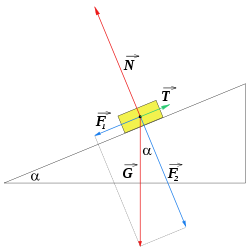
\includegraphics[scale = 0.6]{./img/rownia.PNG}
\caption{Rozkład sił na równi pochyłej.}
\label{fig:rownia}
\end{figure}

Korzystając z tych danych wartość prędkości można obliczyć:

\begin{equation}
E_{P} = E_{K} + E_{T}
\end{equation}
Gdzie:\\
$ E_{P} $ jest wartością energii potencjalnej ciała równej \emph{mgh}.\\
$ E_{K} $ to wartość energii kinetycznej równej $ \frac{mv^{2}}{2} $.\\
$ E_{T} $ jest wartoscią spadku energii spowodowanej tarciem równym $ fmgh \cos
\alpha $.\\
Czyli:\\
\begin{equation}
mgh = \frac{mv^{2}}{2} + fmgh \cos \alpha
\end{equation}
\begin{equation}
\label{eq:boxVelocity}
v(h) = \sqrt{2gh(1-f \cos \alpha)}
\end{equation}
Gdzie \emph{f} jest wspólczynnikiem tarcia ciała o powierzchnię.\\
Dla ciała o kształcie kuli staczjącej się bryle towarzyszy również poślizg, a
siła tarcia nie powoduje opóźnienia staczania się a wprawia ciało w obrót. Aby
ciało poruszało się bez poślizgu przyspieszenie kątowe ($ \varepsilon $) musi
być odpowiednia dla przyspieszenia liniowego staczania (\emph{a}).
\begin{equation}
a = \varepsilon r
\end{equation}
Gdzie \emph{r} jest promeniem kuli. Korzystając z poniższych zależności:
\begin{equation}
a = \frac{F_{1}}{m}
\end{equation}
\begin{equation}
F_{1} = mg \sin \alpha
\end{equation}
Momenty sił ciałą również muszą być zgodne:
\begin{equation}
Tr = I \varepsilon
\end{equation}
Gdzie:\\
\emph{I} to wartość momentu bezwładności kuli równego $ \frac{2}{5}mr^{2} $.\\
\emph{T} jest wartością siły tarcia z rysunku \ref{fig:rownia} równej $ fF_{2}
= fmg \cos \alpha $.
Z tych zależności otrzymać można:
\begin{equation}
f = \frac{2}{5} \tg \alpha
\end{equation}
Przy założeniu że kąt nachylenia równi $ \alpha = 45^{\circ} $ można przyjąć
że:
\begin{equation}
f = \frac{2}{5}
\label{eq:friction}
\end{equation}

W przypadku obliczeń prędkości dla ciała kulistego, przy założeniu że
współczynnik tarcia jest taki jak we wzorze \ref{eq:friction}, energia
potencjalna musi być równa sumie energii kinetycznej liniowej i obrotowej.
\begin{equation}
E_{P} = E_{KL} + E_{KR}
\end{equation}
\begin{equation}
mgh = \frac{mv^{2}}{2} + \frac{I\omega^{2}}{2}
\end{equation}
\begin{equation}
v(h) = \sqrt{\frac{10}{7}gh}
\label{eq:ballVelocity}
\end{equation}
Natomiast uwzględniając wartość współczynnika tarcia z równania
\ref{eq:friction} we wzorze na prędkość zsuwającego się sześcianu -
\ref{eq:boxVelocity}:
\begin{equation}
v(h) = \sqrt{2gh\frac{5-\sqrt{2}}{5}}
\label{eq:ballVelocity2}
\end{equation}

Do przetestowania wartości prędkości ciał na równi pochyłej wykorzystana
zostanie następująca scena:

\lstinputlisting[language=Java, caption=Kod sceny użytaj do testowania prędkości
ciał na równi pochyłej,
label=lis:InclinedPlaneScene]{./listings/InclinedPlaneScene.java}

Z podstawy o długości 30 metrów (ln. 23, 25), staczają się dwa ciała (ln. 26, 
27). Podstawa jest nachylona pod kątem $ 45^{\circ} $ (ln. 30). Współczynnik
tarcia jest zgodny z tym z równania \ref{eq:friction} (ln. 37, 42). Pomiary
wysokości i prędkości ciał są zapisywane w pliku CSV (ln. 42, 50).

\begin{figure}
\centering
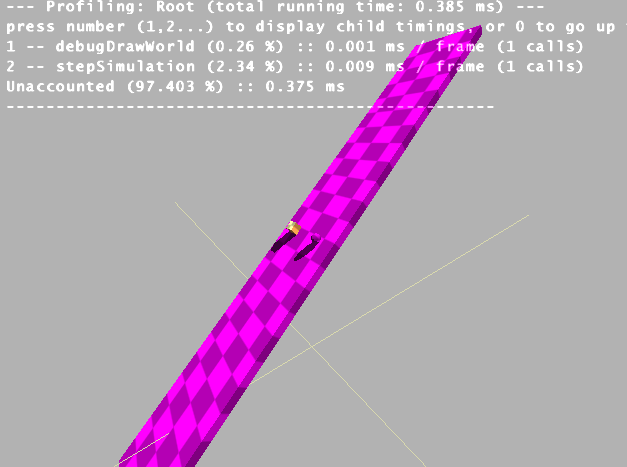
\includegraphics[scale=0.5]{./img/rowniaScreen.PNG}
\caption{Widok staczających się ciał po równi pochyłej.}
\label{fig:rowniaScreen}
\end{figure}

\begin{figure}
\centering
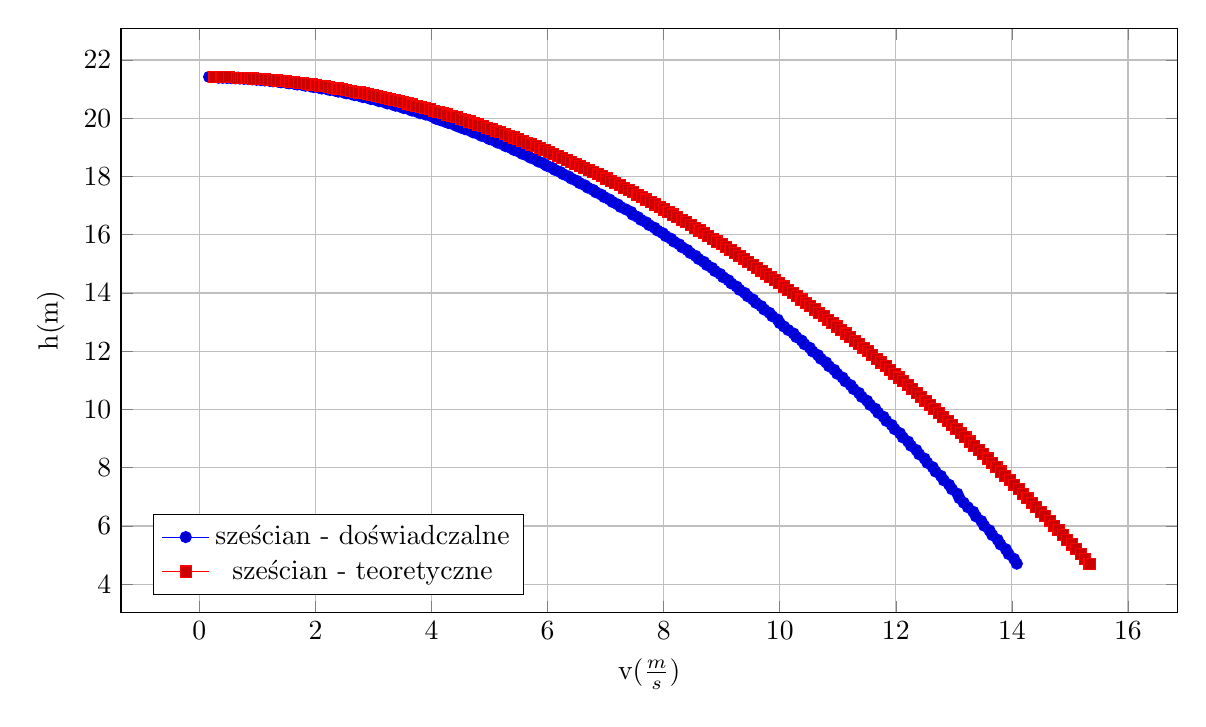
\begin{tikzpicture}
\begin{axis}[
height=9cm,
width=15cm,
grid=major,
xlabel=v($ \frac{m}{s} $),
ylabel=h(m),
legend style = { legend pos = south west }
]
\addplot coordinates { (0.166667, 21.4208) (0.333333, 21.4153) (0.5, 21.407) (0.666667, 21.3958) (0.329325, 21.3932) (0.400907, 21.3895) (0.474289, 21.3847) (0.548032, 21.3788) (0.621608, 21.3719) (0.694828, 21.3641) (0.76764, 21.3554) (0.840098, 21.3457) (0.912216, 21.3351) (0.984064, 21.3237) (1.05569, 21.3114) (1.12712, 21.2982) (1.21191, 21.2836) (1.26699, 21.2688) (1.36111, 21.2523) (1.40569, 21.2359) (1.49936, 21.2178) (1.54543, 21.1999) (1.63885, 21.1802) (1.68579, 21.1606) (1.77907, 21.1393) (1.82653, 21.1181) (1.91974, 21.0951) (1.9675, 21.0723) (2.06066, 21.0476) (2.10858, 21.0231) (2.20172, 20.9968) (2.24977, 20.9707) (2.34289, 20.9427) (2.39098, 20.9149) (2.4841, 20.8853) (2.53222, 20.8558) (2.62534, 20.8245) (2.67349, 20.7934) (2.7666, 20.7605) (2.81476, 20.7276) (2.90786, 20.693) (2.95601, 20.6586) (3.04914, 20.6223) (3.09729, 20.5862) (3.19043, 20.5482) (3.2386, 20.5104) (3.3317, 20.4708) (3.37986, 20.4314) (3.47299, 20.3901) (3.52115, 20.349) (3.61428, 20.3061) (3.66245, 20.2632) (3.75556, 20.2187) (3.80372, 20.1742) (3.89685, 20.128) (3.98742, 20.0801) (4.04696, 20.0318) (4.07563, 19.9845) (4.15039, 19.9361) (4.22448, 19.8867) (4.29189, 19.8366) (4.38664, 19.7846) (4.43713, 19.7326) (4.50521, 19.6798) (4.5774, 19.626) (4.6716, 19.5705) (4.71666, 19.5152) (4.81043, 19.4581) (4.85677, 19.4012) (4.95029, 19.3425) (4.99739, 19.2839) (5.09075, 19.2236) (5.13831, 19.1634) (5.23158, 19.1014) (5.27939, 19.0395) (5.37259, 18.9759) (5.42057, 18.9124) (5.51373, 18.8471) (5.56178, 18.7819) (5.65493, 18.7149) (5.70305, 18.6481) (5.79618, 18.5795) (5.84432, 18.511) (5.93743, 18.4407) (5.9856, 18.3705) (6.07871, 18.2986) (6.12688, 18.2267) (6.21999, 18.1531) (6.26818, 18.0796) (6.36128, 18.0043) (6.40945, 17.9292) (6.50255, 17.8522) (6.55074, 17.7754) (6.64385, 17.6968) (6.69201, 17.6183) (6.78515, 17.538) (6.83332, 17.4579) (6.92642, 17.3759) (6.97459, 17.2941) (7.06772, 17.2105) (7.11588, 17.127) (7.20902, 17.0418) (7.25717, 16.9566) (7.3503, 16.8697) (7.4386, 16.7812) (7.46348, 16.6938) (7.55807, 16.6045) (7.60671, 16.5154) (7.70077, 16.4244) (7.74927, 16.3335) (7.84299, 16.2408) (7.89142, 16.1483) (7.9849, 16.0539) (8.03323, 15.9596) (8.12661, 15.8636) (8.17488, 15.7676) (8.26817, 15.6699) (8.31641, 15.5723) (8.40964, 15.4729) (8.45787, 15.3736) (8.55104, 15.2725) (8.59924, 15.1716) (8.69241, 15.0688) (8.74059, 14.9662) (8.83375, 14.8618) (8.88192, 14.7575) (8.97507, 14.6515) (9.02323, 14.5455) (9.11638, 14.4378) (9.16457, 14.3301) (9.25768, 14.2208) (9.30585, 14.1115) (9.39898, 14.0004) (9.44714, 13.8894) (9.54028, 13.7767) (9.58843, 13.6641) (9.68157, 13.5497) (9.72973, 13.4354) (9.82286, 13.3194) (9.87057, 13.2034) (9.96576, 13.0857) (9.99911, 12.9682) (10.0721, 12.8498) (10.1446, 12.7305) (10.2388, 12.6094) (10.2842, 12.4886) (10.378, 12.3659) (10.4245, 12.2434) (10.5181, 12.1191) (10.5653, 11.995) (10.6587, 11.869) (10.7063, 11.7432) (10.7996, 11.6157) (10.8474, 11.4882) (10.9406, 11.359) (10.9886, 11.2299) (11.0818, 11.099) (11.1299, 10.9682) (11.223, 10.8356) (11.2712, 10.7032) (11.3643, 10.569) (11.4124, 10.4349) (11.5056, 10.299) (11.5537, 10.1632) (11.6468, 10.0257) (11.695, 9.88826) (11.7881, 9.74906) (11.8363, 9.60995) (11.9294, 9.46909) (11.9776, 9.32832) (12.0707, 9.18579) (12.1189, 9.04336) (12.212, 8.89916) (12.2602, 8.75507) (12.3533, 8.60921) (12.4014, 8.46345) (12.4946, 8.31592) (12.5427, 8.1685) (12.6359, 8.01931) (12.684, 7.87022) (12.7772, 7.71937) (12.8253, 7.56861) (12.9185, 7.41609) (12.9663, 7.26368) (13.0611, 7.10944) (13.0951, 6.95551) (13.1681, 6.80066) (13.2406, 6.6449) (13.3348, 6.48733) (13.3802, 6.32998) (13.474, 6.17083) (13.5205, 6.01185) (13.614, 5.8511) (13.6612, 5.69048) (13.7546, 5.52809) (13.8022, 5.36581) (13.8955, 5.20177) (13.9433, 5.03784) (14.0366, 4.87215) (14.0845, 4.70656) };
\addlegendentry{sześcian - doświadczalne}
\addplot coordinates { (0.260638424916547, 21.4208) (0.38118913715862, 21.4153) (0.511959321244021, 21.407) (0.647836916635917, 21.3958) (0.67547931476419, 21.3932) (0.712977718990509, 21.3895) (0.758854796568443, 21.3847) (0.811724154714412, 21.3788) (0.86946400936729, 21.3719) (0.930447958527598, 21.3641) (0.994052135452544, 21.3554) (1.06048839070125, 21.3457) (1.12861512933017, 21.3351) (1.19757270383455, 21.3237) (1.26777600304705, 21.3114) (1.33901908551026, 21.2982) (1.41365266487289, 21.2836) (1.48547861368767, 21.2688) (1.56167176325121, 21.2523) (1.63388135686768, 21.2359) (1.71004590876822, 21.2178) (1.78216940412552, 21.1999) (1.85830740367395, 21.1802) (1.93108505080897, 21.1606) (2.00718999348788, 21.1393) (2.08017102042807, 21.1181) (2.15655260198813, 21.0951) (2.22969407470511, 21.0723) (2.30631360557917, 21.0476) (2.3798763163062, 21.0231) (2.45639467488067, 20.9968) (2.53004355096511, 20.9707) (2.6067405278718, 20.9427) (2.68071894137555, 20.9149) (2.75730785185138, 20.8853) (2.83157495837279, 20.8558) (2.90830679635196, 20.8245) (2.98258869341248, 20.7934) (3.05920853991164, 20.7605) (3.13395572196939, 20.7276) (3.21068720616994, 20.693) (3.28520244356146, 20.6586) (3.36204225038478, 20.6223) (3.43675083576105, 20.5862) (3.51367921092645, 20.5482) (3.58856641858837, 20.5104) (3.66538005780779, 20.4708) (3.74023997209549, 20.4314) (3.81713365870492, 20.3901) (3.8921466751789, 20.349) (3.96893396241682, 20.3061) (4.04426357387167, 20.2632) (4.12094839196358, 20.2187) (4.1962320531054, 20.1742) (4.27298765851171, 20.128) (4.3511403959961, 20.0801) (4.42854728073367, 20.0318) (4.50306002129365, 19.9845) (4.57805419579396, 19.9361) (4.65335081211763, 19.8867) (4.72848990026325, 19.8366) (4.80523567913361, 19.7846) (4.88077484905273, 19.7326) (4.95629713315892, 19.6798) (5.03208596424164, 19.626) (5.10909085091256, 19.5705) (5.18468046723905, 19.5152) (5.26159181770054, 19.4581) (5.3371310100041, 19.4012) (5.41395365942891, 19.3425) (5.48957669751406, 19.2839) (5.5663179808333, 19.2236) (5.64189186842206, 19.1634) (5.71868223723063, 19.1014) (5.79433461678108, 19.0395) (5.87104643368207, 18.9759) (5.94665368796802, 18.9124) (6.02341280250977, 18.8471) (6.0990893666206, 18.7819) (6.17589199520449, 18.7149) (6.25152365318881, 18.6481) (6.32825321242432, 18.5795) (6.40395455168902, 18.511) (6.48072425939265, 18.4407) (6.5564887247537, 18.3705) (6.63319236860774, 18.2986) (6.70901712343174, 18.2267) (6.78575859102253, 18.1531) (6.86153817715407, 18.0796) (6.93831588655929, 18.0043) (7.01405236507043, 17.9292) (7.09086483139331, 17.8522) (7.16665749058527, 17.7754) (7.24340595313177, 17.6968) (7.31925436514729, 17.6183) (7.39603589554788, 17.538) (7.47184169836715, 17.4579) (7.54865505662867, 17.3759) (7.62451158128789, 17.2941) (7.70126407734879, 17.2105) (7.7771694317594, 17.127) (7.85386525738214, 17.0418) (7.92981763689093, 16.9566) (8.00654452040143, 16.8697) (8.08393421916378, 16.7812) (8.15964284212052, 16.6938) (8.23627831007679, 16.6045) (8.31203774920718, 16.5154) (8.38870627250234, 16.4244) (8.46459796763882, 16.3335) (8.54129688208018, 16.2408) (8.61715121096468, 16.1483) (8.69388105487411, 16.0539) (8.76985850557115, 15.9596) (8.84653648321024, 15.8636) (8.92255478386131, 15.7676) (8.99926028649244, 15.6699) (9.07523986259531, 15.5723) (9.15197206555367, 15.4729) (9.22799064038703, 15.3736) (9.30474884641726, 15.2725) (9.38072880877957, 15.1716) (9.45751228021918, 15.0688) (9.53352957357647, 14.9662) (9.61026300344869, 14.8618) (9.68631654995913, 14.7575) (9.76300229993683, 14.6515) (9.83909038027051, 14.5455) (9.9158003915818, 14.4378) (9.99192217338838, 14.3301) (10.0685859658134, 14.2208) (10.144671083958, 14.1115) (10.2214285067132, 14.0004) (10.2975453900709, 13.8894) (10.3742562960096, 13.7767) (10.4503373522283, 13.6641) (10.5270712508703, 13.5497) (10.6031834131541, 13.4354) (10.6798732939988, 13.3194) (10.7560163935702, 13.2034) (10.8327280051535, 13.0857) (10.908771648561, 12.9682) (10.9848648444384, 12.8498) (11.0610071766918, 12.7305) (11.1377663182214, 12.6094) (11.2138115926513, 12.4886) (11.2905284442549, 12.3659) (11.3666041603243, 12.2434) (11.4432805169632, 12.1191) (11.5193241943896, 11.995) (11.5960217764483, 11.869) (11.6720952556171, 11.7432) (11.7486943948395, 11.6157) (11.8247967801427, 11.4882) (11.9014177101222, 11.359) (11.9774896850931, 11.2299) (12.0541324651111, 11.099) (12.1302329261619, 10.9682) (12.2068961437738, 10.8356) (12.2829661784093, 10.7032) (12.3595929342047, 10.569) (12.4356908889336, 10.4349) (12.5123384287351, 10.299) (12.5884627986529, 10.1632) (12.6650747112098, 10.0257) (12.7411922693729, 9.88826) (12.8178240955548, 9.74906) (12.893951056932, 9.60995) (12.9705804288261, 9.46909) (13.0467119043395, 9.32832) (13.1233444908793, 9.18579) (13.1994793148484, 9.04336) (13.2761150041696, 8.89916) (13.3522535656786, 8.75507) (13.4288872519068, 8.60921) (13.5050339278819, 8.46345) (13.5816710556417, 8.31592) (13.6578211788665, 8.1685) (13.7344557710502, 8.01931) (13.8106141183708, 7.87022) (13.8872466825144, 7.71937) (13.9634130401555, 7.56861) (14.0400483665057, 7.41609) (14.1162127593372, 7.26368) (14.1928756024562, 7.10944) (14.2689735177086, 6.95551) (14.3451190921563, 6.80066) (14.4213066858271, 6.6449) (14.4979720460483, 6.48733) (14.574128012926, 6.32998) (14.6507525131355, 6.17083) (14.7268970190702, 6.01185) (14.8034910646866, 5.8511) (14.8796292940633, 5.69048) (14.9562127608376, 5.52809) (15.0323545226739, 5.36581) (15.108932100871, 5.20177) (15.1850724756692, 5.03784) (15.2616443196461, 4.87215) (15.3377879635236, 4.70656) };
\addlegendentry{sześcian - teoretyczne}
\end{axis}
\end{tikzpicture}
\caption{Wykres zależności prędkości od wysokości dla ciała o kształcie
sześcianu.}
\label{fig:boxDiagram}
\end{figure}

\begin{figure}
\centering
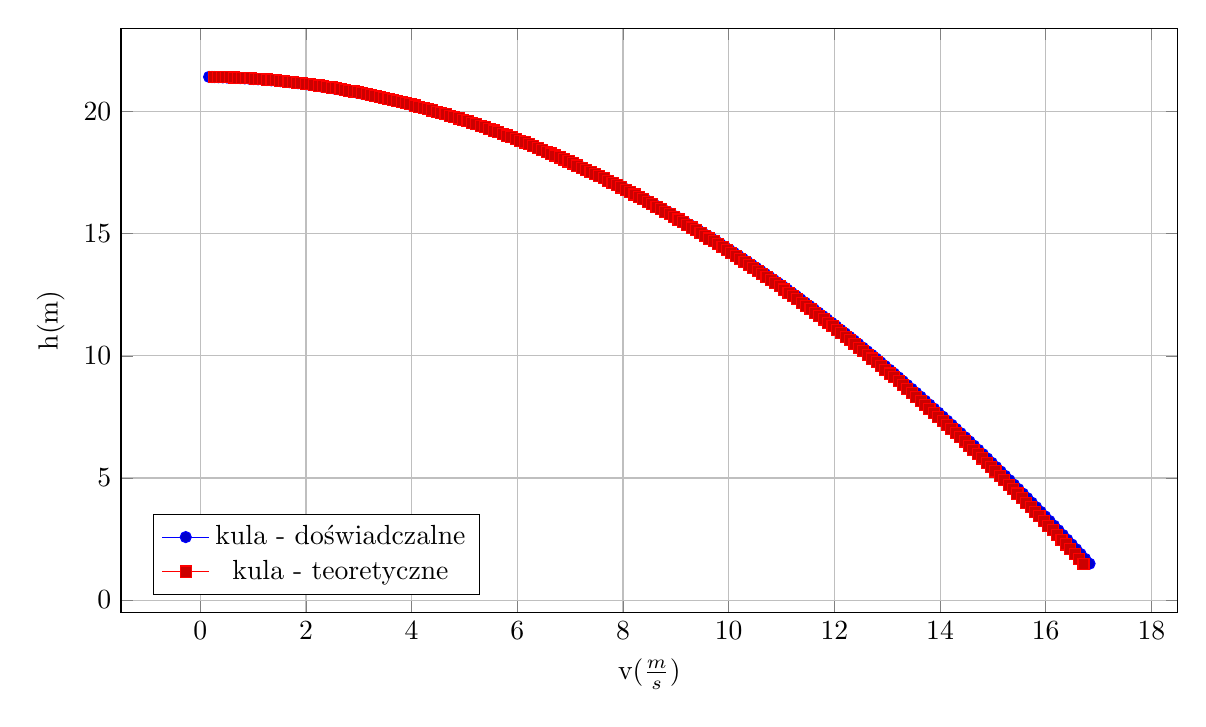
\begin{tikzpicture}
\begin{axis}[
height=9cm,
width=15cm,
grid=major,
xlabel=v($ \frac{m}{s} $),
ylabel=h(m),
legend style = { legend pos = south west }
]
\addplot coordinates { (0.166667, 21.4208) (0.222576, 21.4172) (0.26957, 21.4131) (0.34498, 21.4083) (0.425059, 21.4026) (0.507191, 21.3961) (0.590292, 21.3887) (0.67388, 21.3804) (0.757718, 21.3712) (0.841693, 21.361) (0.925741, 21.35) (1.00983, 21.3379) (1.09394, 21.3249) (1.17806, 21.3109) (1.2622, 21.296) (1.34632, 21.2801) (1.43045, 21.2632) (1.5146, 21.2453) (1.59874, 21.2264) (1.68288, 21.2066) (1.76702, 21.1857) (1.85117, 21.1639) (1.93531, 21.1411) (2.01946, 21.1173) (2.1036, 21.0925) (2.18775, 21.0667) (2.27189, 21.04) (2.35604, 21.0122) (2.44019, 20.9834) (2.52433, 20.9537) (2.60848, 20.923) (2.69262, 20.8912) (2.77677, 20.8585) (2.86092, 20.8248) (2.94506, 20.7901) (3.02921, 20.7544) (3.11335, 20.7178) (3.1975, 20.6801) (3.28164, 20.6414) (3.36579, 20.6018) (3.44994, 20.5612) (3.53408, 20.5195) (3.61823, 20.4769) (3.70237, 20.4333) (3.78652, 20.3887) (3.87066, 20.3431) (3.95481, 20.2965) (4.03896, 20.2489) (4.12311, 20.2003) (4.20725, 20.1508) (4.29139, 20.1002) (4.37554, 20.0487) (4.45969, 19.9961) (4.54383, 19.9426) (4.62798, 19.8881) (4.71212, 19.8326) (4.79627, 19.7761) (4.88042, 19.7186) (4.96456, 19.6601) (5.04871, 19.6006) (5.13286, 19.5402) (5.217, 19.4787) (5.30114, 19.4162) (5.38529, 19.3528) (5.46944, 19.2884) (5.55359, 19.2229) (5.63774, 19.1565) (5.72187, 19.0891) (5.80602, 19.0207) (5.89016, 18.9513) (5.97431, 18.881) (6.05846, 18.8096) (6.1426, 18.7372) (6.22675, 18.6639) (6.3109, 18.5895) (6.39504, 18.5142) (6.47918, 18.4379) (6.56333, 18.3605) (6.64748, 18.2822) (6.73162, 18.2029) (6.81577, 18.1226) (6.89992, 18.0414) (6.98406, 17.9591) (7.06821, 17.8758) (7.15236, 17.7916) (7.2365, 17.7063) (7.32064, 17.6201) (7.40479, 17.5328) (7.48893, 17.4446) (7.57308, 17.3554) (7.65723, 17.2652) (7.74138, 17.174) (7.82551, 17.0818) (7.90967, 16.9886) (7.99381, 16.8945) (8.07796, 16.7993) (8.1621, 16.7031) (8.24624, 16.606) (8.33039, 16.5079) (8.41454, 16.4087) (8.49868, 16.3086) (8.58283, 16.2075) (8.66698, 16.1054) (8.75113, 16.0023) (8.83527, 15.8982) (8.91942, 15.7932) (9.00356, 15.6871) (9.08771, 15.58) (9.17186, 15.472) (9.25599, 15.363) (9.34014, 15.2529) (9.42429, 15.1419) (9.50844, 15.0299) (9.59258, 14.9169) (9.67673, 14.8029) (9.76087, 14.6879) (9.84502, 14.5719) (9.92916, 14.4549) (10.0133, 14.337) (10.0975, 14.218) (10.1816, 14.0981) (10.2657, 13.9772) (10.3499, 13.8552) (10.434, 13.7323) (10.5182, 13.6084) (10.6023, 13.4835) (10.6865, 13.3576) (10.7706, 13.2307) (10.8548, 13.1029) (10.9389, 12.974) (11.0231, 12.8441) (11.1072, 12.7133) (11.1913, 12.5814) (11.2755, 12.4486) (11.3596, 12.3148) (11.4438, 12.18) (11.5279, 12.0442) (11.6121, 11.9074) (11.6962, 11.7696) (11.7804, 11.6308) (11.8645, 11.4911) (11.9487, 11.3503) (12.0328, 11.2086) (12.117, 11.0658) (12.2011, 10.9221) (12.2852, 10.7774) (12.3694, 10.6316) (12.4535, 10.4849) (12.5377, 10.3372) (12.6218, 10.1885) (12.706, 10.0389) (12.7901, 9.88818) (12.8742, 9.73652) (12.9584, 9.58386) (13.0425, 9.43022) (13.1267, 9.27558) (13.2108, 9.11995) (13.295, 8.96333) (13.3791, 8.80571) (13.4633, 8.64711) (13.5474, 8.48751) (13.6316, 8.32693) (13.7157, 8.16535) (13.7999, 8.00278) (13.884, 7.83923) (13.9681, 7.67468) (14.0523, 7.50914) (14.1364, 7.3426) (14.2206, 7.17507) (14.3047, 7.00655) (14.3889, 6.83704) (14.473, 6.66655) (14.5572, 6.49506) (14.6413, 6.32257) (14.7255, 6.1491) (14.8096, 5.97464) (14.8938, 5.79918) (14.9779, 5.62274) (15.062, 5.44531) (15.1462, 5.26688) (15.2303, 5.08746) (15.3145, 4.90705) (15.3986, 4.72565) (15.4828, 4.54325) (15.5669, 4.35987) (15.6511, 4.17549) (15.7352, 3.99012) (15.8194, 3.80377) (15.9035, 3.61642) (15.9876, 3.42807) (16.0718, 3.23874) (16.1559, 3.04842) (16.2401, 2.8571) (16.3242, 2.6648) (16.4084, 2.4715) (16.4925, 2.27721) (16.5767, 2.08193) (16.6608, 1.88565) (16.745, 1.68839) (16.8291, 1.49014) };
\addlegendentry{kula - doświadczalne}
\addplot coordinates { (0.260116089681703, 21.4208) (0.343656999001204, 21.4172) (0.419010631918851, 21.4131) (0.492770649960662, 21.4083) (0.568083856607408, 21.4026) (0.64328496542145, 21.3961) (0.719375921165622, 21.3887) (0.796135187039345, 21.3804) (0.873355967946484, 21.3712) (0.951684493421651, 21.361) (1.02949309235893, 21.35) (1.10879753051151, 21.3379) (1.18811805847192, 21.3249) (1.26799986810053, 21.3109) (1.34782767106327, 21.296) (1.4280972598888, 21.2801) (1.50873812305423, 21.2632) (1.58970216763343, 21.2453) (1.67093441733566, 21.2264) (1.75200093979435, 21.2066) (1.83368918939439, 21.1857) (1.91518006573265, 21.1639) (1.99685919449107, 21.1411) (2.0786979550922, 21.1173) (2.16067820876287, 21.0925) (2.24279039874592, 21.0667) (2.32471011401578, 21.04) (2.40705119806259, 21.0122) (2.48947658821897, 20.9834) (2.57171834526253, 20.9537) (2.65404534036965, 20.923) (2.73671849200876, 20.8912) (2.81920014026742, 20.8585) (2.90175073786537, 20.8248) (2.98436904153733, 20.7901) (3.06704522218176, 20.7544) (3.14955406914605, 20.7178) (3.2323425805906, 20.6801) (3.31517614457527, 20.6414) (3.397843002765, 20.6018) (3.48056623568807, 20.5612) (3.56352569719728, 20.5195) (3.64633141925313, 20.4769) (3.72917642796864, 20.4333) (3.81205816196954, 20.3887) (3.89497770816807, 20.3431) (3.97792934218934, 20.2965) (4.06091109767413, 20.2489) (4.14392116508171, 20.2003) (4.22679345631607, 20.1508) (4.30986154146032, 20.1002) (4.39279486335363, 20.0487) (4.47591445413242, 19.9961) (4.55889938258494, 19.9426) (4.64191235138289, 19.8881) (4.72494905398417, 19.8326) (4.80800826070506, 19.7761) (4.89109155760104, 19.7186) (4.97419236378859, 19.6601) (5.05731774429923, 19.6006) (5.14032350657538, 19.5402) (5.22348401852904, 19.4787) (5.30666356093649, 19.4162) (5.38972982874457, 19.3528) (5.47281496966452, 19.2884) (5.55604562992127, 19.2229) (5.63916651750021, 19.1565) (5.72230386906016, 19.0891) (5.80545697728125, 19.0207) (5.88862744430585, 18.9513) (5.97169369033752, 18.881) (6.05489398493978, 18.8096) (6.1381096539626, 18.7372) (6.22122407327481, 18.6639) (6.30446596469339, 18.5895) (6.38761065272499, 18.5142) (6.47076928881499, 18.4379) (6.55404942089965, 18.3605) (6.63723504592565, 18.2822) (6.72043308764916, 18.2029) (6.80364309055911, 18.1226) (6.88676370602338, 18.0414) (6.96999947386993, 17.9591) (7.05324778428061, 17.8758) (7.13640706783097, 17.7916) (7.2196747796037, 17.7063) (7.30285871146206, 17.6201) (7.38614807257737, 17.5328) (7.46935503851391, 17.4446) (7.55257081330698, 17.3554) (7.63579860959059, 17.2652) (7.71903630707047, 17.174) (7.80228358885754, 17.0818) (7.88554184629092, 16.9886) (7.9687201675596, 16.8945) (8.05199863527831, 16.7993) (8.13528381763568, 16.7031) (8.21849257377478, 16.606) (8.30171252781396, 16.5079) (8.38502463668801, 16.4087) (8.46826362202666, 16.3086) (8.55150976399629, 16.2075) (8.63476595125042, 16.1054) (8.71803036295817, 16.0023) (8.8013035249643, 15.8982) (8.88450621522561, 15.7932) (8.96779539197597, 15.6871) (9.05109336013469, 15.58) (9.13432159993744, 15.472) (9.21755884824148, 15.363) (9.30087958580798, 15.2529) (9.38413275904329, 15.1419) (9.46739426460633, 15.0299) (9.55066318488352, 14.9169) (9.63393932761232, 14.8029) (9.71722388250405, 14.6879) (9.80051458953415, 14.5719) (9.88381332149703, 14.4549) (9.96704813796008, 14.337) (10.0503602579121, 14.218) (10.133610611674, 14.0981) (10.2168680784125, 13.9772) (10.3002006074411, 13.8552) (10.3834718854591, 13.7323) (10.4667497737429, 13.6084) (10.5500353825824, 13.4835) (10.6333266452088, 13.3576) (10.7166253004964, 13.2307) (10.7998649701953, 13.1029) (10.8831759535927, 12.974) (10.9664932522556, 12.8441) (11.0497532229195, 12.7133) (11.1330826028674, 12.5814) (11.2163553268368, 12.4486) (11.2996341525241, 12.3148) (11.3829195330732, 12.18) (11.4662113256495, 12.0442) (11.5495088129289, 11.9074) (11.632812447035, 11.7696) (11.7161215264823, 11.6308) (11.799377036075, 11.4911) (11.8826982011606, 11.3503) (11.9659658154266, 11.2086) (12.0492980101045, 11.0658) (12.1325772378477, 10.9221) (12.2158625680249, 10.7774) (12.2992103831343, 10.6316) (12.3825066298012, 10.4849) (12.465808629128, 10.3372) (12.5491157340449, 10.1885) (12.6323728276048, 10.0389) (12.7157022910798, 9.88818) (12.7990035097863, 9.73652) (12.8823097121248, 9.58386) (12.9656110093549, 9.43022) (13.04891671347, 9.27558) (13.132222669682, 9.11995) (13.2155283675657, 8.96333) (13.2988393393656, 8.80571) (13.3821445006273, 8.64711) (13.4654548771879, 8.48751) (13.5487595219852, 8.32693) (13.6320693246508, 8.16535) (13.7153788316757, 8.00278) (13.7986829633952, 7.83923) (13.881991925591, 7.67468) (13.9653008467194, 7.50914) (14.0486144842315, 7.3426) (14.1319277896022, 7.17507) (14.2152407686713, 7.00655) (14.2985534271427, 6.83704) (14.3818608917633, 6.66655) (14.4651731847119, 6.49506) (14.5484899933758, 6.32257) (14.6318016496473, 6.1491) (14.7151130093751, 5.97464) (14.7984288190575, 5.79918) (14.8817397985884, 5.62274) (14.9650502707919, 5.44531) (15.0483653509035, 5.26688) (15.1316801049324, 5.08746) (15.2149945382356, 4.90705) (15.2983088744604, 4.72565) (15.3816272424502, 4.54325) (15.4649409348736, 4.35987) (15.5482588376494, 4.17549) (15.631576394681, 3.99012) (15.7148891464933, 3.80377) (15.798206157714, 3.61642) (15.881527256113, 3.42807) (15.9648436922062, 3.23874) (16.0481598067592, 3.04842) (16.1314799544232, 2.8571) (16.2147955214217, 2.6648) (16.2981150858941, 2.4715) (16.3814343035454, 2.27721) (16.464753281108, 2.08193) (16.5480761109404, 1.88565) (16.6313944479734, 1.68839) (16.7147125073126, 1.49014) };
\addlegendentry{kula - teoretyczne}
\end{axis}
\end{tikzpicture}
\caption{Wykres zależności prędkości od wysokości dla ciała o kształcie
kuli.}
\label{fig:ballDiagram}
\end{figure}

Zestawienie doświadczalnych pomiarów prędkości i teoretycznych wyników
obliczonych ze wzorów \ref{eq:boxVelocity} dla sześcianu i
\ref{eq:ballVelocity2} dla kuli przedstawiają wykresy na rysunkach
\ref{fig:boxDiagram} i \ref{fig:ballDiagram}. Różnica wyników na wykresie jest
niewielka, co potwierdza stwierdzenie z końca testu z sekcji
\ref{sec:odbicieWieluCial}: przy obecnym tarciu i braku sprężystości wynik
symulacji ma niski odstęp od teoretycznego.

\subsubsection{Kołyska Newtona}
W tym teście, tak jak w poprzednim, sprawdzona zostanie zasada zachowania
energii zarówno przy braniu pod uwagę energii kinetycznej jak i potencjalnej.
Z tą różnicą, że brana pod uwagę będzie również sprężystość ciał tak jak w
sekcjach \ref{sec:odbicie1ciala} i \ref{sec:odbicieWieluCial}. W celu
przeprowadzenia tego testu zostanie użyta poniższa scena:

\lstinputlisting[language=Java, caption=Kod sceny użytaj do testowania
zachowania energii dla kołyski Newtona,
label=lis:NewtonPendulumScene]{./listings/NewtonPendulumLogScene.java}

Scena składa się z czterech kulek (ln. 24-33) zawieszonych na nierozciągliwych
niciach (ln. 37-42). Kulka położona najbardziej z lewej strony posiada prędkość
początkową (ln. 35), która wprawia w ruch wahadło. Podobnie jak w przypadku
testu z sekcji \ref{sec:odbicie1ciala} przeprowadzone zostało 10 testów dla
różnych wartości współczynnika spręzystości zmienijącego się od 0,99 do 0,91
(ln.
73-81). Wynik testu przedstawiono na rysunku \ref{fig:wahadloNewtona1}.

\begin{figure}
\centering
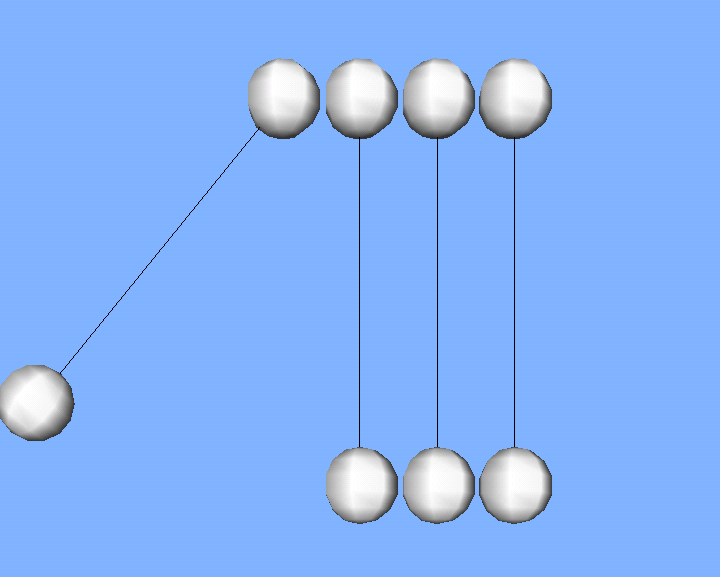
\includegraphics[scale=0.5]{img/newtonPendulum.png}
\caption{Wizulalizacja symulacji wahadła Newtona.}
\label{fig:newtonPendulum}
\end{figure}

\begin{figure}
\centering
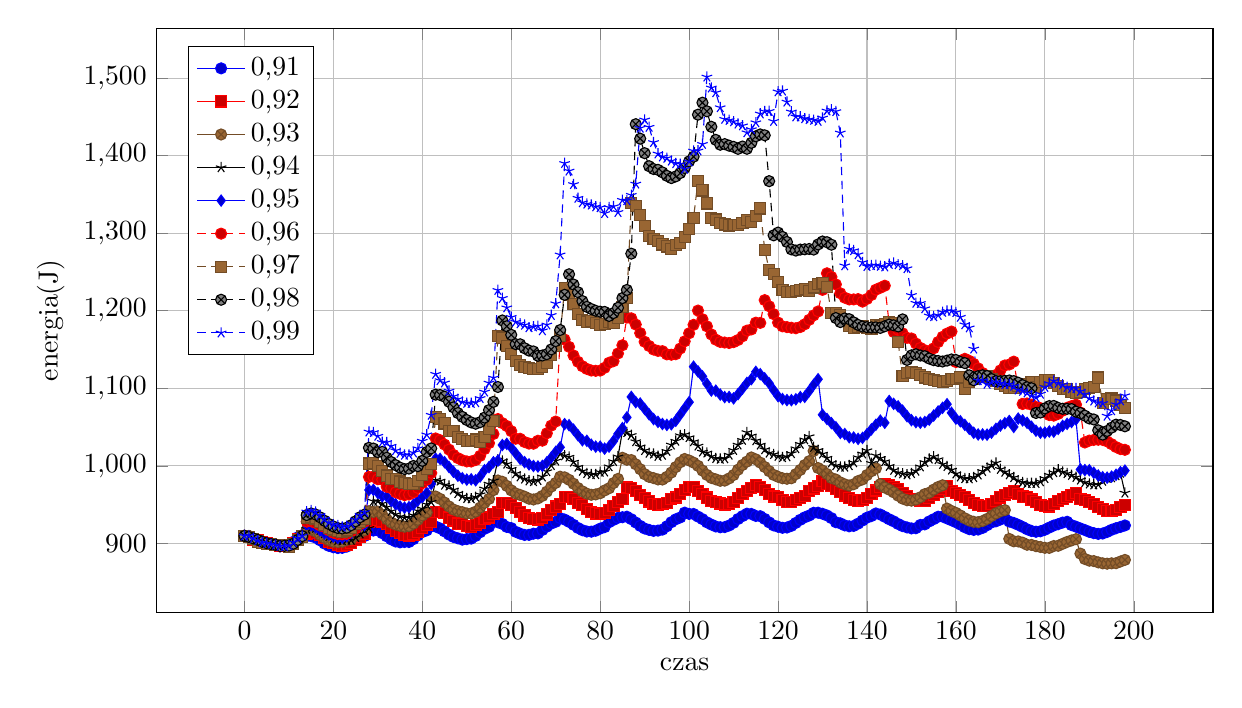
\begin{tikzpicture}
\begin{axis}[
height=9cm,
width=15cm,
grid=major,
ylabel=energia(J),
xlabel=czas,
legend style = { legend pos = north west }
]
\addplot coordinates {(0, 909.70496) (1, 908.91003) (2, 905.84564) (3, 902.58923) (4, 900.7118) (5, 899.6155) (6, 898.84607) (7, 897.6105) (8, 896.1678) (9, 896.5277) (10, 898.22107) (11, 901.9944) (12, 907.8563) (13, 908.8547) (14, 909.2997) (15, 909.3721) (16, 907.3194) (17, 903.9783) (18, 899.7727) (19, 896.734) (20, 894.93964) (21, 893.91846) (22, 894.23486) (23, 895.80505) (24, 900.08563) (25, 904.24927) (26, 907.3873) (27, 909.39166) (28, 917.235) (29, 916.4924) (30, 916.7624) (31, 913.0932) (32, 909.07275) (33, 905.1402) (34, 902.4144) (35, 901.29126) (36, 901.8047) (37, 901.7821) (38, 905.3781) (39, 910.1511) (40, 914.522) (41, 916.7622) (42, 922.2126) (43, 921.65985) (44, 919.28204) (45, 915.4203) (46, 911.3654) (47, 908.3199) (48, 906.4784) (49, 904.80896) (50, 905.4777) (51, 906.15204) (52, 909.5542) (53, 914.283) (54, 918.73975) (55, 921.3679) (56, 927.81757) (57, 927.17566) (58, 925.04126) (59, 921.2051) (60, 919.69714) (61, 914.90155) (62, 912.5438) (63, 910.86884) (64, 910.9824) (65, 912.49304) (66, 912.831) (67, 917.26294) (68, 921.5398) (69, 925.4276) (70, 927.76245) (71, 932.54865) (72, 930.6869) (73, 927.719) (74, 923.94104) (75, 919.88763) (76, 916.99927) (77, 915.2503) (78, 915.06055) (79, 916.30615) (80, 919.01013) (81, 920.91956) (82, 927.2283) (83, 930.27673) (84, 932.9399) (85, 933.68164) (86, 934.36096) (87, 931.192) (88, 926.8906) (89, 922.56604) (90, 919.1821) (91, 917.35754) (92, 916.07043) (93, 916.4395) (94, 917.73584) (95, 922.01874) (96, 927.2545) (97, 931.03644) (98, 933.3866) (99, 939.61084) (100, 938.0183) (101, 937.9207) (102, 934.5193) (103, 931.2433) (104, 927.11597) (105, 924.24384) (106, 921.79504) (107, 920.7748) (108, 920.95575) (109, 923.05756) (110, 926.51263) (111, 931.3986) (112, 935.10925) (113, 938.28455) (114, 937.90283) (115, 935.384) (116, 935.0177) (117, 931.53174) (118, 927.0408) (119, 923.1942) (120, 921.41693) (121, 920.0447) (122, 920.3994) (123, 922.54565) (124, 926.36786) (125, 930.36755) (126, 933.5651) (127, 935.90283) (128, 939.4008) (129, 939.542) (130, 938.13824) (131, 935.99084) (132, 932.5513) (133, 927.2705) (134, 925.82025) (135, 923.1827) (136, 921.99207) (137, 922.48706) (138, 925.44824) (139, 929.4689) (140, 933.16003) (141, 935.2602) (142, 938.57715) (143, 937.1677) (144, 934.2166) (145, 931.0611) (146, 928.3711) (147, 925.0017) (148, 922.24005) (149, 920.5496) (150, 919.3118) (151, 919.5635) (152, 923.7449) (153, 924.4903) (154, 928.2876) (155, 931.21796) (156, 934.3411) (157, 934.55066) (158, 932.1289) (159, 929.72925) (160, 927.2245) (161, 924.19244) (162, 920.79895) (163, 918.32385) (164, 917.34424) (165, 917.80634) (166, 919.92786) (167, 923.3916) (168, 926.9508) (169, 928.404) (170, 930.7395) (171, 932.5349) (172, 928.1836) (173, 926.364) (174, 923.9332) (175, 921.21735) (176, 918.21594) (177, 915.9688) (178, 914.9617) (179, 915.54236) (180, 917.5162) (181, 920.3622) (182, 922.9785) (183, 924.78864) (184, 926.80237) (185, 927.8245) (186, 923.56177) (187, 921.49524) (188, 919.2682) (189, 917.1438) (190, 914.8053) (191, 913.173) (192, 912.20135) (193, 912.6698) (194, 914.7105) (195, 917.4619) (196, 919.5323) (197, 921.1834) (198, 923.1088) };
\addlegendentry{0,91}
\addplot coordinates {(0, 909.1787) (1, 908.13934) (2, 904.5642) (3, 904.20984) (4, 901.753) (5, 900.4624) (6, 899.1829) (7, 897.99994) (8, 897.1827) (9, 896.64624) (10, 897.5131) (11, 900.32465) (12, 905.9315) (13, 908.63446) (14, 911.9656) (15, 913.8413) (16, 913.6787) (17, 911.23267) (18, 906.43195) (19, 902.1035) (20, 900.41187) (21, 897.87) (22, 896.98413) (23, 897.4239) (24, 900.0449) (25, 904.07306) (26, 908.64795) (27, 911.743) (28, 928.1131) (29, 928.30554) (30, 929.86487) (31, 928.25085) (32, 924.7457) (33, 920.0731) (34, 916.05786) (35, 912.8404) (36, 910.75867) (37, 910.2098) (38, 911.48596) (39, 914.6422) (40, 919.3395) (41, 924.2844) (42, 927.7405) (43, 940.8048) (44, 940.41345) (45, 939.29016) (46, 933.27026) (47, 929.49677) (48, 925.565) (49, 924.4775) (50, 922.09796) (51, 921.7048) (52, 923.2141) (53, 926.18195) (54, 931.4317) (55, 933.3411) (56, 938.2189) (57, 939.93713) (58, 951.9556) (59, 952.02405) (60, 949.7427) (61, 945.3213) (62, 940.5553) (63, 935.9614) (64, 932.8647) (65, 930.8993) (66, 930.8019) (67, 933.1334) (68, 937.27075) (69, 942.682) (70, 947.4635) (71, 950.31287) (72, 960.0233) (73, 959.2642) (74, 956.83484) (75, 951.5177) (76, 949.04047) (77, 944.4262) (78, 940.8878) (79, 938.5813) (80, 937.8515) (81, 939.1008) (82, 942.8586) (83, 947.94653) (84, 953.2825) (85, 957.4925) (86, 972.0305) (87, 970.8919) (88, 967.3214) (89, 962.85284) (90, 958.2051) (91, 954.01996) (92, 951.25665) (93, 949.91534) (94, 950.29736) (95, 951.97504) (96, 957.0646) (97, 959.1543) (98, 963.8471) (99, 968.5325) (100, 972.4231) (101, 972.2938) (102, 967.91797) (103, 963.34094) (104, 959.1086) (105, 954.8698) (106, 953.8247) (107, 951.47675) (108, 950.12134) (109, 950.9726) (110, 953.7616) (111, 958.6757) (112, 964.04034) (113, 967.5072) (114, 970.9823) (115, 974.8054) (116, 972.5266) (117, 968.43933) (118, 963.90466) (119, 960.4289) (120, 959.6368) (121, 955.9646) (122, 953.5905) (123, 953.3126) (124, 955.60626) (125, 958.2536) (126, 961.4951) (127, 967.1506) (128, 970.8456) (129, 973.6851) (130, 979.95734) (131, 976.6576) (132, 974.001) (133, 970.1766) (134, 965.9596) (135, 961.7529) (136, 958.5348) (137, 955.93964) (138, 954.77234) (139, 955.428) (140, 958.689) (141, 963.3363) (142, 968.1599) (143, 972.33887) (144, 976.1632) (145, 975.74744) (146, 972.7854) (147, 969.77625) (148, 965.2561) (149, 961.1616) (150, 957.69385) (151, 955.5743) (152, 955.2931) (153, 954.64716) (154, 958.62) (155, 962.30096) (156, 966.8022) (157, 970.6934) (158, 973.50964) (159, 967.91907) (160, 965.2726) (161, 962.51697) (162, 959.40894) (163, 955.54736) (164, 951.95605) (165, 949.74255) (166, 948.3175) (167, 948.65967) (168, 950.9596) (169, 954.84656) (170, 959.19604) (171, 962.2247) (172, 965.2717) (173, 967.43494) (174, 963.37225) (175, 960.365) (176, 959.9951) (177, 956.5266) (178, 952.8398) (179, 949.4498) (180, 948.3187) (181, 947.5949) (182, 950.3111) (183, 954.2063) (184, 957.6494) (185, 960.25665) (186, 962.7656) (187, 964.5305) (188, 957.57916) (189, 955.4142) (190, 952.8511) (191, 950.401) (192, 947.14545) (193, 943.99335) (194, 942.0585) (195, 941.8961) (196, 943.445) (197, 946.7905) (198, 949.78766) };
\addlegendentry{0,92}
\addplot coordinates {(0, 909.9739) (1, 909.6043) (2, 904.7189) (3, 903.0693) (4, 901.36316) (5, 900.247) (6, 898.8993) (7, 897.92426) (8, 897.0292) (9, 897.62115) (10, 896.2848) (11, 899.8707) (12, 905.5753) (13, 910.0138) (14, 917.0958) (15, 917.80774) (16, 915.3461) (17, 911.2122) (18, 907.3193) (19, 904.1981) (20, 902.2132) (21, 901.6106) (22, 902.1876) (23, 904.3843) (24, 905.47797) (25, 910.21924) (26, 914.87024) (27, 916.8254) (28, 941.40015) (29, 940.4674) (30, 940.9399) (31, 936.8323) (32, 931.1941) (33, 926.89453) (34, 924.2845) (35, 922.6271) (36, 921.4746) (37, 922.2319) (38, 925.4561) (39, 930.3051) (40, 936.0466) (41, 939.86127) (42, 960.3177) (43, 960.43317) (44, 957.38403) (45, 952.62823) (46, 947.63336) (47, 943.67773) (48, 941.5397) (49, 940.20447) (50, 938.60046) (51, 938.5745) (52, 940.90106) (53, 946.08405) (54, 952.2277) (55, 957.3572) (56, 968.6071) (57, 981.08875) (58, 979.407) (59, 974.1169) (60, 968.3111) (61, 964.45374) (62, 962.4042) (63, 960.24023) (64, 957.5823) (65, 956.563) (66, 957.9829) (67, 961.21704) (68, 966.6929) (69, 973.1835) (70, 977.9487) (71, 985.98834) (72, 985.13135) (73, 981.9289) (74, 976.91174) (75, 971.3896) (76, 967.0934) (77, 964.1389) (78, 962.6211) (79, 963.11127) (80, 964.64264) (81, 968.20105) (82, 971.0374) (83, 977.7105) (84, 983.132) (85, 1010.3999) (86, 1007.7708) (87, 1007.3976) (88, 1001.9574) (89, 995.6572) (90, 989.22864) (91, 985.7379) (92, 984.15027) (93, 982.4234) (94, 982.3069) (95, 985.8097) (96, 991.3164) (97, 998.313) (98, 1004.5246) (99, 1008.808) (100, 1006.88586) (101, 1004.11676) (102, 999.93353) (103, 993.82086) (104, 988.3091) (105, 984.36804) (106, 982.5341) (107, 980.68713) (108, 980.88855) (109, 983.73315) (110, 988.1511) (111, 995.01135) (112, 1001.0484) (113, 1005.4299) (114, 1010.75104) (115, 1008.3402) (116, 1004.1299) (117, 998.49097) (118, 993.12726) (119, 988.3389) (120, 985.8577) (121, 983.9355) (122, 983.28204) (123, 983.97705) (124, 989.28375) (125, 994.7015) (126, 1000.9625) (127, 1005.9709) (128, 1019.1315) (129, 997.17456) (130, 993.9058) (131, 989.45355) (132, 984.26196) (133, 982.3118) (134, 978.65784) (135, 976.1677) (136, 974.5676) (137, 976.25635) (138, 980.3346) (139, 982.4793) (140, 988.1001) (141, 993.02136) (142, 996.6898) (143, 976.29895) (144, 971.9361) (145, 969.2471) (146, 965.8012) (147, 961.49634) (148, 957.7179) (149, 955.60657) (150, 955.079) (151, 956.43317) (152, 959.43066) (153, 963.4711) (154, 965.3247) (155, 969.3207) (156, 972.6736) (157, 974.90875) (158, 944.8591) (159, 941.8281) (160, 939.3228) (161, 935.9552) (162, 932.2947) (163, 929.4629) (164, 927.81085) (165, 927.3264) (166, 928.8199) (167, 931.52734) (168, 935.214) (169, 938.66595) (170, 941.3007) (171, 942.9132) (172, 905.74164) (173, 902.6578) (174, 902.5233) (175, 900.9094) (176, 898.18396) (177, 897.9547) (178, 896.4235) (179, 895.332) (180, 894.2488) (181, 894.1743) (182, 896.56396) (183, 896.88257) (184, 899.3873) (185, 901.81934) (186, 903.7855) (187, 905.39374) (188, 886.78015) (189, 879.84705) (190, 877.67084) (191, 877.1596) (192, 875.4732) (193, 874.2599) (194, 873.793) (195, 874.2577) (196, 874.449) (197, 876.6093) (198, 878.65784) };
\addlegendentry{0,93}
\addplot coordinates {(0, 909.67334) (1, 909.7395) (2, 906.58405) (3, 903.32104) (4, 901.14734) (5, 900.1527) (6, 899.1553) (7, 898.2587) (8, 897.50366) (9, 897.53577) (10, 895.7014) (11, 899.9214) (12, 902.62573) (13, 908.53394) (14, 918.3235) (15, 920.24664) (16, 919.68616) (17, 916.9132) (18, 912.69073) (19, 908.8165) (20, 905.9721) (21, 904.0185) (22, 903.86646) (23, 904.32587) (24, 904.20905) (25, 907.6812) (26, 912.3648) (27, 916.94934) (28, 919.5088) (29, 954.4324) (30, 954.5701) (31, 951.27484) (32, 946.5541) (33, 941.42554) (34, 937.3576) (35, 934.4773) (36, 933.1264) (37, 933.506) (38, 936.2306) (39, 941.89264) (40, 944.5719) (41, 950.3117) (42, 953.2987) (43, 981.74207) (44, 980.5242) (45, 975.2261) (46, 974.0681) (47, 969.01825) (48, 964.4431) (49, 960.63696) (50, 958.02057) (51, 957.61395) (52, 959.6751) (53, 962.98425) (54, 970.3402) (55, 976.66846) (56, 980.7751) (57, 1007.93524) (58, 1006.3307) (59, 1002.36865) (60, 995.7335) (61, 989.98145) (62, 985.89166) (63, 983.1045) (64, 980.7224) (65, 979.8093) (66, 981.2403) (67, 985.79517) (68, 992.6531) (69, 1000.6193) (70, 1006.2992) (71, 1015.39404) (72, 1013.0596) (73, 1011.3426) (74, 1004.95374) (75, 998.47363) (76, 993.24) (77, 990.1861) (78, 988.78467) (79, 988.91266) (80, 991.86975) (81, 992.23456) (82, 998.9504) (83, 1005.683) (84, 1011.7738) (85, 1044.3723) (86, 1043.0721) (87, 1039.3811) (88, 1031.309) (89, 1024.6162) (90, 1019.83734) (91, 1016.4575) (92, 1015.3943) (93, 1012.3496) (94, 1013.82605) (95, 1018.9554) (96, 1026.9794) (97, 1031.962) (98, 1039.0825) (99, 1040.269) (100, 1036.5806) (101, 1031.2874) (102, 1025.6825) (103, 1017.94226) (104, 1016.67725) (105, 1012.0706) (106, 1009.5895) (107, 1008.7506) (108, 1009.37836) (109, 1013.96466) (110, 1020.1177) (111, 1026.9619) (112, 1033.0669) (113, 1043.1077) (114, 1038.7488) (115, 1032.4875) (116, 1026.9181) (117, 1020.91406) (118, 1016.588) (119, 1014.7702) (120, 1012.3839) (121, 1010.7206) (122, 1011.79456) (123, 1015.91125) (124, 1022.27234) (125, 1027.9658) (126, 1033.7383) (127, 1037.8134) (128, 1023.9173) (129, 1020.0767) (130, 1015.3577) (131, 1010.02783) (132, 1003.9313) (133, 1000.3403) (134, 998.4502) (135, 998.5117) (136, 1000.3926) (137, 1004.2471) (138, 1010.72833) (139, 1015.5627) (140, 1019.7233) (141, 1003.369) (142, 1013.2262) (143, 1009.7943) (144, 1005.5122) (145, 999.5055) (146, 994.3635) (147, 991.0992) (148, 989.8928) (149, 988.5348) (150, 990.2317) (151, 993.30945) (152, 998.8373) (153, 1004.52264) (154, 1008.8589) (155, 1011.90576) (156, 1008.1788) (157, 1001.9394) (158, 999.2472) (159, 994.72) (160, 989.68854) (161, 985.81104) (162, 983.6238) (163, 983.3953) (164, 984.9821) (165, 988.35876) (166, 992.96277) (167, 997.1659) (168, 1000.82886) (169, 1003.78796) (170, 995.6111) (171, 991.99146) (172, 988.5641) (173, 984.9553) (174, 980.7616) (175, 978.6859) (176, 977.3955) (177, 977.57904) (178, 977.43726) (179, 979.6384) (180, 983.8006) (181, 988.0523) (182, 991.3484) (183, 994.8977) (184, 991.9836) (185, 990.1166) (186, 987.884) (187, 985.2417) (188, 981.8419) (189, 978.56165) (190, 976.77905) (191, 975.5905) (192, 975.81995) (193, 980.32776) (194, 984.0427) (195, 984.71564) (196, 987.4054) (197, 990.64777) (198, 965.0211) };
\addlegendentry{0,94}
\addplot coordinates {(0, 909.5659) (1, 908.6117) (2, 905.4626) (3, 901.4686) (4, 901.5639) (5, 900.2623) (6, 899.0072) (7, 898.0794) (8, 897.0696) (9, 897.12866) (10, 898.5479) (11, 901.2849) (12, 906.84973) (13, 910.3592) (14, 923.6178) (15, 923.32007) (16, 920.6079) (17, 916.85077) (18, 912.8082) (19, 911.4247) (20, 908.5945) (21, 906.87555) (22, 907.21716) (23, 909.2346) (24, 913.44836) (25, 918.34784) (26, 922.15485) (27, 923.49976) (28, 968.8397) (29, 969.0267) (30, 964.97546) (31, 960.7023) (32, 960.52625) (33, 954.8468) (34, 950.5472) (35, 947.4741) (36, 946.05304) (37, 946.65063) (38, 949.8723) (39, 955.40247) (40, 959.68005) (41, 965.02966) (42, 976.6876) (43, 1009.29) (44, 1008.9318) (45, 1004.71606) (46, 998.5113) (47, 992.3855) (48, 987.24243) (49, 984.0341) (50, 982.2018) (51, 982.6046) (52, 981.3457) (53, 986.1884) (54, 994.42413) (55, 998.2281) (56, 1004.58105) (57, 1006.71155) (58, 1026.8196) (59, 1028.2837) (60, 1023.46094) (61, 1016.24426) (62, 1009.0635) (63, 1004.7899) (64, 1001.8331) (65, 999.81433) (66, 999.14636) (67, 999.94995) (68, 1004.40295) (69, 1010.68964) (70, 1017.9617) (71, 1023.84595) (72, 1053.8132) (73, 1052.42) (74, 1046.6638) (75, 1039.4769) (76, 1032.9218) (77, 1032.2646) (78, 1027.2319) (79, 1024.726) (80, 1024.6979) (81, 1022.087) (82, 1024.6869) (83, 1032.0337) (84, 1041.0902) (85, 1048.6495) (86, 1062.4413) (87, 1088.8953) (88, 1082.0835) (89, 1080.3743) (90, 1073.3544) (91, 1066.3971) (92, 1060.2471) (93, 1056.6511) (94, 1053.8882) (95, 1052.7085) (96, 1053.551) (97, 1058.0192) (98, 1066.023) (99, 1074.107) (100, 1082.0973) (101, 1127.866) (102, 1121.6584) (103, 1115.3148) (104, 1105.78) (105, 1097.0294) (106, 1096.9288) (107, 1091.8207) (108, 1088.6364) (109, 1088.7241) (110, 1086.9429) (111, 1092.4435) (112, 1099.505) (113, 1106.8649) (114, 1111.7421) (115, 1121.2185) (116, 1118.1719) (117, 1112.805) (118, 1106.4553) (119, 1097.6644) (120, 1089.8394) (121, 1086.0743) (122, 1084.7351) (123, 1084.6259) (124, 1085.746) (125, 1088.6382) (126, 1088.981) (127, 1096.3613) (128, 1104.4028) (129, 1111.6569) (130, 1065.8538) (131, 1060.4138) (132, 1055.0598) (133, 1049.7157) (134, 1042.448) (135, 1040.9706) (136, 1036.8711) (137, 1036.4187) (138, 1034.7344) (139, 1035.9993) (140, 1040.703) (141, 1047.074) (142, 1052.9779) (143, 1058.239) (144, 1055.526) (145, 1083.6028) (146, 1079.873) (147, 1076.6838) (148, 1071.0828) (149, 1063.9832) (150, 1058.8601) (151, 1056.381) (152, 1055.5848) (153, 1056.5137) (154, 1059.532) (155, 1064.7682) (156, 1070.0176) (157, 1074.7877) (158, 1079.4548) (159, 1068.3157) (160, 1060.8453) (161, 1057.488) (162, 1052.7922) (163, 1047.7703) (164, 1042.6177) (165, 1040.4645) (166, 1040.4508) (167, 1040.1252) (168, 1042.7137) (169, 1047.7) (170, 1051.9172) (171, 1054.9749) (172, 1057.8097) (173, 1050.1525) (174, 1060.9108) (175, 1058.5652) (176, 1055.5043) (177, 1050.312) (178, 1045.2546) (179, 1042.7438) (180, 1042.7281) (181, 1044.2651) (182, 1044.0206) (183, 1047.565) (184, 1051.5272) (185, 1054.1058) (186, 1056.5005) (187, 1059.7993) (188, 995.36536) (189, 994.478) (190, 994.3211) (191, 991.01416) (192, 987.50226) (193, 985.29803) (194, 984.74316) (195, 986.06256) (196, 988.4034) (197, 991.7284) (198, 993.8518) };
\addlegendentry{0,95}
\addplot coordinates {(0, 909.4227) (1, 908.0355) (2, 904.4029) (3, 904.0963) (4, 901.78204) (5, 899.977) (6, 899.31165) (7, 898.1444) (8, 896.14746) (9, 897.63855) (10, 896.5153) (11, 899.58325) (12, 905.1875) (13, 909.65283) (14, 928.06335) (15, 928.5551) (16, 926.3002) (17, 923.08765) (18, 921.30676) (19, 916.786) (20, 913.7089) (21, 911.90576) (22, 911.6773) (23, 912.31354) (24, 915.5513) (25, 919.07214) (26, 924.66547) (27, 927.9022) (28, 985.68427) (29, 986.09424) (30, 982.71686) (31, 982.1249) (32, 973.0176) (33, 971.2328) (34, 965.974) (35, 963.7964) (36, 962.12366) (37, 962.9886) (38, 965.7911) (39, 971.41064) (40, 977.57324) (41, 982.06415) (42, 990.8093) (43, 1035.2825) (44, 1033.0834) (45, 1027.4497) (46, 1020.9534) (47, 1014.11127) (48, 1009.9263) (49, 1007.18427) (50, 1005.65515) (51, 1005.56805) (52, 1007.4956) (53, 1012.87494) (54, 1021.5216) (55, 1029.2517) (56, 1041.0073) (57, 1060.3477) (58, 1055.0491) (59, 1051.3777) (60, 1044.6804) (61, 1034.9203) (62, 1034.8405) (63, 1030.7124) (64, 1028.6354) (65, 1028.4932) (66, 1032.2869) (67, 1032.4194) (68, 1041.9034) (69, 1051.8398) (70, 1057.0684) (71, 1163.698) (72, 1162.8722) (73, 1153.4343) (74, 1142.3119) (75, 1134.1791) (76, 1128.3998) (77, 1124.974) (78, 1122.8567) (79, 1122.492) (80, 1122.7874) (81, 1126.4161) (82, 1132.8763) (83, 1134.969) (84, 1144.8694) (85, 1155.4626) (86, 1191.1631) (87, 1190.1875) (88, 1182.1843) (89, 1171.1655) (90, 1159.9847) (91, 1154.5552) (92, 1149.9521) (93, 1148.1661) (94, 1147.8401) (95, 1143.7131) (96, 1143.2509) (97, 1143.9551) (98, 1151.2417) (99, 1160.5322) (100, 1170.8994) (101, 1181.8037) (102, 1200.1886) (103, 1189.0424) (104, 1179.8473) (105, 1169.4008) (106, 1162.6785) (107, 1159.7471) (108, 1158.976) (109, 1158.3854) (110, 1159.4841) (111, 1162.2518) (112, 1166.959) (113, 1174.3123) (114, 1175.894) (115, 1184.6056) (116, 1184.282) (117, 1213.6726) (118, 1205.7495) (119, 1195.5991) (120, 1184.7273) (121, 1179.8691) (122, 1178.8672) (123, 1178.0403) (124, 1177.3843) (125, 1178.9359) (126, 1182.4617) (127, 1188.2639) (128, 1193.963) (129, 1199.024) (130, 1226.904) (131, 1248.2544) (132, 1243.5195) (133, 1233.894) (134, 1222.5508) (135, 1216.8026) (136, 1214.5361) (137, 1214.6079) (138, 1214.9906) (139, 1211.7329) (140, 1215.1731) (141, 1220.2906) (142, 1227.1106) (143, 1229.575) (144, 1232.2747) (145, 1182.903) (146, 1172.644) (147, 1175.4806) (148, 1170.8922) (149, 1165.0874) (150, 1164.208) (151, 1157.6741) (152, 1152.0853) (153, 1148.9987) (154, 1147.7932) (155, 1151.4775) (156, 1159.647) (157, 1166.2854) (158, 1170.5328) (159, 1173.1443) (160, 1133.8182) (161, 1135.099) (162, 1137.9657) (163, 1135.349) (164, 1131.4375) (165, 1125.689) (166, 1119.6802) (167, 1115.8015) (168, 1114.3916) (169, 1117.102) (170, 1123.033) (171, 1129.374) (172, 1130.6432) (173, 1134.3253) (174, 1100.6993) (175, 1079.6891) (176, 1080.3911) (177, 1078.7491) (178, 1075.9617) (179, 1074.4453) (180, 1069.2336) (181, 1065.4521) (182, 1064.7241) (183, 1066.9835) (184, 1071.0712) (185, 1074.8881) (186, 1076.9812) (187, 1078.8992) (188, 1068.7571) (189, 1030.0558) (190, 1032.4908) (191, 1033.4059) (192, 1033.6274) (193, 1033.4037) (194, 1031.459) (195, 1027.9617) (196, 1024.239) (197, 1021.5959) (198, 1020.6255) };
\addlegendentry{0,96}
\addplot coordinates {(0, 909.76276) (1, 908.7257) (2, 905.2697) (3, 902.34814) (4, 900.6684) (5, 899.69727) (6, 899.02594) (7, 898.3128) (8, 897.4695) (9, 897.4558) (10, 895.7705) (11, 899.13525) (12, 904.50964) (13, 908.75745) (14, 932.70996) (15, 934.25867) (16, 932.1585) (17, 927.86804) (18, 923.3109) (19, 919.8789) (20, 917.91455) (21, 915.5646) (22, 914.8242) (23, 916.6098) (24, 919.5702) (25, 924.9909) (26, 928.10266) (27, 931.9929) (28, 1002.89886) (29, 1003.7047) (30, 1000.24396) (31, 993.72754) (32, 987.468) (33, 983.2019) (34, 982.5575) (35, 979.66235) (36, 977.9791) (37, 976.6222) (38, 976.8895) (39, 980.4007) (40, 988.39795) (41, 996.4884) (42, 1002.24615) (43, 1063.2979) (44, 1060.5295) (45, 1054.6448) (46, 1045.3641) (47, 1045.1565) (48, 1036.6825) (49, 1034.8069) (50, 1032.5065) (51, 1032.0701) (52, 1033.8235) (53, 1031.2139) (54, 1037.2216) (55, 1047.9626) (56, 1057.8234) (57, 1167.1692) (58, 1165.4084) (59, 1154.6729) (60, 1143.9316) (61, 1135.2651) (62, 1130.4144) (63, 1127.875) (64, 1126.2688) (65, 1125.0642) (66, 1125.3705) (67, 1127.5745) (68, 1133.1066) (69, 1143.1432) (70, 1154.5378) (71, 1167.6177) (72, 1229.5071) (73, 1220.7107) (74, 1208.1985) (75, 1195.2644) (76, 1187.7162) (77, 1186.0667) (78, 1186.7856) (79, 1183.7413) (80, 1181.5376) (81, 1182.5925) (82, 1185.2628) (83, 1183.8586) (84, 1190.8306) (85, 1205.201) (86, 1216.339) (87, 1338.9896) (88, 1335.2594) (89, 1322.9409) (90, 1309.332) (91, 1296.8368) (92, 1292.115) (93, 1289.4481) (94, 1285.4602) (95, 1282.8547) (96, 1280.0599) (97, 1284.7739) (98, 1287.6216) (99, 1295.1493) (100, 1305.0857) (101, 1319.8671) (102, 1367.8025) (103, 1355.1328) (104, 1338.3766) (105, 1319.1506) (106, 1317.5986) (107, 1313.2175) (108, 1311.2174) (109, 1309.9934) (110, 1310.4152) (111, 1310.5837) (112, 1313.3341) (113, 1317.3209) (114, 1314.3865) (115, 1321.918) (116, 1331.9265) (117, 1278.6373) (118, 1252.6865) (119, 1247.541) (120, 1237.5605) (121, 1226.7831) (122, 1223.8013) (123, 1224.4473) (124, 1225.7396) (125, 1227.023) (126, 1228.2867) (127, 1225.7399) (128, 1230.0283) (129, 1234.9126) (130, 1235.9805) (131, 1230.9746) (132, 1196.5745) (133, 1196.8346) (134, 1194.2894) (135, 1187.0034) (136, 1180.5488) (137, 1178.146) (138, 1179.3134) (139, 1179.6887) (140, 1177.4318) (141, 1177.1201) (142, 1181.9897) (143, 1180.7834) (144, 1182.4023) (145, 1185.4158) (146, 1183.9424) (147, 1160.0151) (148, 1115.5726) (149, 1119.7395) (150, 1121.218) (151, 1120.0708) (152, 1116.9832) (153, 1113.9795) (154, 1111.9436) (155, 1110.5731) (156, 1109.426) (157, 1108.4067) (158, 1109.4465) (159, 1111.5796) (160, 1111.9263) (161, 1113.9095) (162, 1098.8013) (163, 1108.4921) (164, 1111.5061) (165, 1114.0454) (166, 1114.5731) (167, 1115.1782) (168, 1112.3136) (169, 1109.1401) (170, 1105.8082) (171, 1103.0586) (172, 1100.7346) (173, 1100.6083) (174, 1102.4788) (175, 1103.7638) (176, 1105.4498) (177, 1107.9178) (178, 1102.0347) (179, 1108.351) (180, 1110.9196) (181, 1110.2266) (182, 1107.1418) (183, 1102.648) (184, 1099.5278) (185, 1098.8271) (186, 1095.481) (187, 1093.8972) (188, 1095.5612) (189, 1098.5359) (190, 1100.053) (191, 1102.0377) (192, 1113.8347) (193, 1080.7711) (194, 1085.8274) (195, 1086.6931) (196, 1084.1442) (197, 1078.8319) (198, 1074.0748) };
\addlegendentry{0,97}
\addplot coordinates {(0, 909.6168) (1, 908.2284) (2, 906.353) (3, 904.44806) (4, 901.96027) (5, 900.2355) (6, 899.0921) (7, 898.06384) (8, 896.55444) (9, 896.8848) (10, 897.14954) (11, 899.5578) (12, 904.49304) (13, 909.3315) (14, 936.5219) (15, 938.56195) (16, 937.22577) (17, 933.5965) (18, 929.15643) (19, 924.9546) (20, 921.80914) (21, 919.74396) (22, 919.14355) (23, 920.228) (24, 923.3823) (25, 928.50256) (26, 933.739) (27, 937.02356) (28, 1023.22974) (29, 1022.2643) (30, 1017.6314) (31, 1017.9916) (32, 1010.36743) (33, 1004.8505) (34, 1000.8524) (35, 997.701) (36, 995.7185) (37, 996.45166) (38, 999.817) (39, 999.5344) (40, 1006.4186) (41, 1017.7843) (42, 1022.4595) (43, 1091.7946) (44, 1091.3389) (45, 1089.1439) (46, 1082.6504) (47, 1075.3701) (48, 1068.0201) (49, 1063.1166) (50, 1059.0372) (51, 1055.9578) (52, 1054.2716) (53, 1056.2751) (54, 1062.1866) (55, 1071.8975) (56, 1082.4574) (57, 1101.6252) (58, 1187.4297) (59, 1179.9447) (60, 1168.9248) (61, 1156.8857) (62, 1156.7285) (63, 1151.6089) (64, 1148.5653) (65, 1147.4626) (66, 1141.9451) (67, 1142.2592) (68, 1143.9657) (69, 1150.1359) (70, 1160.7653) (71, 1175.1246) (72, 1220.4937) (73, 1246.999) (74, 1233.8104) (75, 1223.8809) (76, 1212.4586) (77, 1204.9951) (78, 1202.1577) (79, 1199.8838) (80, 1198.7815) (81, 1198.4749) (82, 1193.2584) (83, 1197.002) (84, 1203.7981) (85, 1216.3052) (86, 1226.7808) (87, 1273.6033) (88, 1440.5541) (89, 1421.8591) (90, 1403.1462) (91, 1386.3732) (92, 1382.6937) (93, 1381.6638) (94, 1378.4099) (95, 1373.9177) (96, 1371.0149) (97, 1373.2296) (98, 1377.4899) (99, 1384.0273) (100, 1392.6204) (101, 1398.6096) (102, 1452.8246) (103, 1468.2661) (104, 1457.156) (105, 1437.1694) (106, 1420.3171) (107, 1414.0574) (108, 1414.8613) (109, 1412.7983) (110, 1411.3054) (111, 1408.7234) (112, 1411.7139) (113, 1408.8191) (114, 1416.4971) (115, 1424.9174) (116, 1427.3481) (117, 1426.1904) (118, 1367.0533) (119, 1297.2026) (120, 1300.7593) (121, 1295.1953) (122, 1288.6527) (123, 1279.0823) (124, 1277.5625) (125, 1278.8253) (126, 1279.1831) (127, 1279.6062) (128, 1278.8384) (129, 1285.4834) (130, 1289.2445) (131, 1288.3655) (132, 1285.1372) (133, 1190.525) (134, 1185.3453) (135, 1190.0532) (136, 1189.0883) (137, 1184.9718) (138, 1181.6843) (139, 1179.5339) (140, 1178.7839) (141, 1178.4363) (142, 1178.504) (143, 1177.827) (144, 1179.9795) (145, 1182.1262) (146, 1181.144) (147, 1179.706) (148, 1188.8461) (149, 1136.5862) (150, 1142.4391) (151, 1143.8334) (152, 1142.2041) (153, 1141.3428) (154, 1138.2974) (155, 1136.1995) (156, 1135.1882) (157, 1134.5187) (158, 1135.7007) (159, 1137.1511) (160, 1136.49) (161, 1133.848) (162, 1132.4353) (163, 1116.7053) (164, 1110.3677) (165, 1115.5997) (166, 1116.6937) (167, 1115.7537) (168, 1111.8313) (169, 1109.1226) (170, 1108.9695) (171, 1109.6768) (172, 1110.069) (173, 1109.1788) (174, 1107.2068) (175, 1103.9441) (176, 1101.2615) (177, 1099.9979) (178, 1068.1345) (179, 1068.7429) (180, 1074.0507) (181, 1077.0673) (182, 1077.1952) (183, 1074.7063) (184, 1073.5518) (185, 1073.4949) (186, 1073.1777) (187, 1069.7738) (188, 1068.0459) (189, 1064.6226) (190, 1061.047) (191, 1059.7603) (192, 1045.8171) (193, 1040.235) (194, 1044.938) (195, 1049.1809) (196, 1053.0927) (197, 1052.6537) (198, 1050.9205) };
\addlegendentry{0,98}
\addplot coordinates {(0, 909.5878) (1, 909.86426) (2, 906.61487) (3, 903.47174) (4, 901.1106) (5, 900.17926) (6, 899.10596) (7, 897.91425) (8, 896.385) (9, 895.9644) (10, 897.32184) (11, 901.3136) (12, 906.7695) (13, 909.67145) (14, 940.80115) (15, 942.6177) (16, 940.51575) (17, 936.24225) (18, 931.48065) (19, 926.78265) (20, 924.1872) (21, 923.07355) (22, 921.12384) (23, 922.3075) (24, 925.2097) (25, 930.5648) (26, 936.30945) (27, 940.08655) (28, 1043.8456) (29, 1043.1482) (30, 1038.3755) (31, 1030.3694) (32, 1030.2524) (33, 1025.4717) (34, 1019.69495) (35, 1016.3958) (36, 1013.927) (37, 1014.1522) (38, 1016.85583) (39, 1022.35925) (40, 1031.927) (41, 1040.1753) (42, 1065.4141) (43, 1118.2289) (44, 1110.0997) (45, 1107.1206) (46, 1096.5522) (47, 1089.6611) (48, 1086.008) (49, 1082.4227) (50, 1080.824) (51, 1080.6755) (52, 1081.6749) (53, 1087.066) (54, 1095.3872) (55, 1106.856) (56, 1113.4546) (57, 1226.4355) (58, 1216.1006) (59, 1203.9604) (60, 1191.6399) (61, 1185.5327) (62, 1183.3264) (63, 1181.5918) (64, 1178.2869) (65, 1179.3514) (66, 1180.1426) (67, 1174.327) (68, 1181.839) (69, 1194.1208) (70, 1209.181) (71, 1272.1914) (72, 1390.1411) (73, 1380.294) (74, 1362.9778) (75, 1345.263) (76, 1339.4382) (77, 1337.6555) (78, 1336.5186) (79, 1334.1448) (80, 1333.1558) (81, 1325.5181) (82, 1333.1868) (83, 1334.4235) (84, 1326.915) (85, 1342.5574) (86, 1342.0848) (87, 1349.0454) (88, 1363.5325) (89, 1435.5681) (90, 1446.1962) (91, 1436.7928) (92, 1417.1343) (93, 1402.4011) (94, 1398.5272) (95, 1396.8397) (96, 1393.1448) (97, 1389.8848) (98, 1389.002) (99, 1382.7485) (100, 1392.2574) (101, 1406.1196) (102, 1406.2717) (103, 1414.7502) (104, 1501.519) (105, 1487.4448) (106, 1481.3555) (107, 1462.0494) (108, 1447.062) (109, 1445.6846) (110, 1443.8536) (111, 1440.8623) (112, 1438.6505) (113, 1429.7037) (114, 1433.7399) (115, 1442.6702) (116, 1453.9675) (117, 1457.0398) (118, 1457.3049) (119, 1444.3408) (120, 1482.4495) (121, 1483.4668) (122, 1469.2418) (123, 1456.5594) (124, 1450.1501) (125, 1450.1671) (126, 1447.8193) (127, 1446.7319) (128, 1445.7227) (129, 1444.3948) (130, 1448.7417) (131, 1457.8057) (132, 1459.196) (133, 1456.9968) (134, 1429.4104) (135, 1258.0933) (136, 1279.5435) (137, 1277.653) (138, 1272.3827) (139, 1262.3793) (140, 1257.1724) (141, 1258.4075) (142, 1258.6066) (143, 1257.584) (144, 1256.6857) (145, 1259.9623) (146, 1261.6577) (147, 1259.4811) (148, 1258.2532) (149, 1254.4366) (150, 1219.8915) (151, 1209.8914) (152, 1209.5901) (153, 1202.7401) (154, 1193.4678) (155, 1192.5352) (156, 1194.1931) (157, 1198.1676) (158, 1199.625) (159, 1199.6345) (160, 1197.9133) (161, 1191.7251) (162, 1182.1095) (163, 1178.0972) (164, 1150.7867) (165, 1109.9576) (166, 1109.9514) (167, 1105.3665) (168, 1107.4327) (169, 1108.3044) (170, 1106.5272) (171, 1104.9205) (172, 1105.1136) (173, 1102.8704) (174, 1097.9751) (175, 1096.2654) (176, 1094.1279) (177, 1090.388) (178, 1088.068) (179, 1092.6411) (180, 1101.3547) (181, 1106.2067) (182, 1109.4713) (183, 1106.6857) (184, 1104.5474) (185, 1101.2765) (186, 1099.7373) (187, 1099.6664) (188, 1096.1567) (189, 1092.303) (190, 1087.0928) (191, 1083.7216) (192, 1081.3608) (193, 1080.4891) (194, 1064.2827) (195, 1071.2083) (196, 1079.1019) (197, 1084.0316) (198, 1090.6111) };
\addlegendentry{0,99}
\end{axis}
\end{tikzpicture}

\caption{Wykres zależności energii od czasu dla wahadła Newtona.}
\label{fig:wahadloNewtona1}
\end{figure}

Z wykresu wynika, że wartość współczynnika sprężystości przy którym całkowita
energia się nie zmienia jest niższa niż 0,91. W celu zwiększenia precyzji
obliczeń test został powtórzony dla wartości od 0,94 do 0,87, dla dwukrotnie
większego odstępu czasu. Jego wynik przedstawia wykres na rysunku
\ref{fig:wahadloNewtona2}.

\begin{figure}
\centering
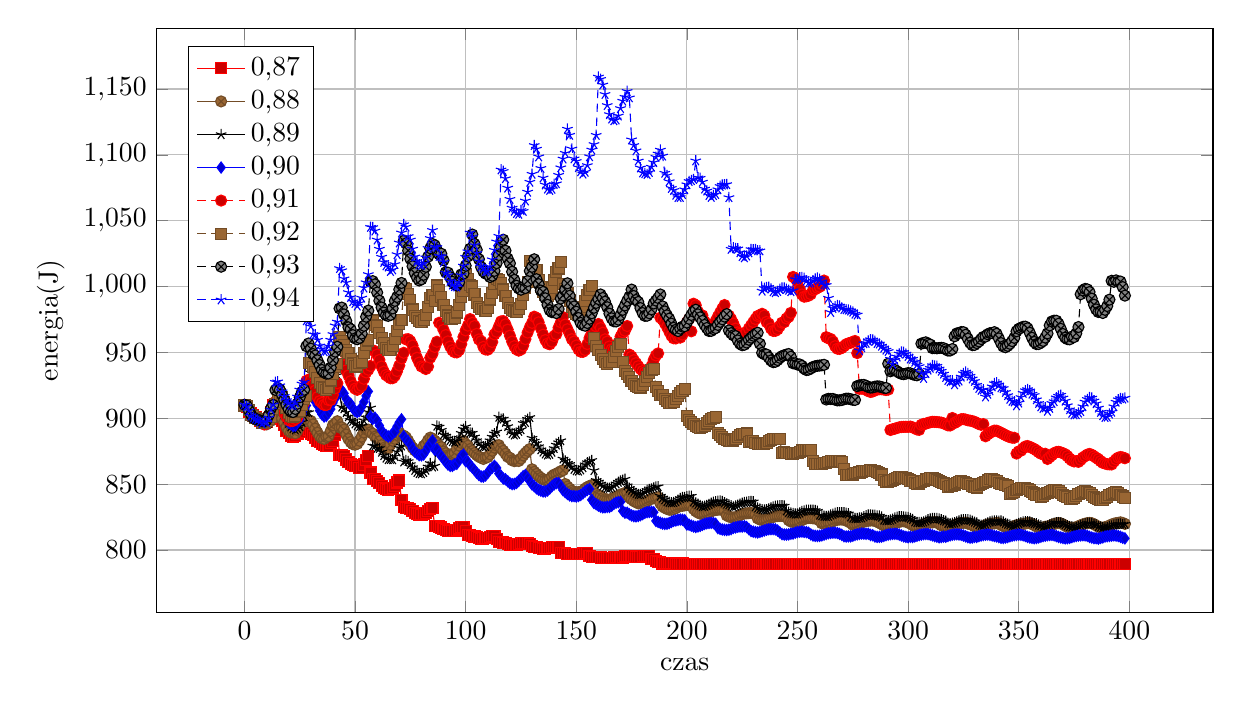
\begin{tikzpicture}
\begin{axis}[
height=9cm,
width=15cm,
grid=major,
ylabel=energia(J),
xlabel=czas,
legend style = { legend pos = north west }
]
\addplot coordinates {};
\addlegendentry{0,87}
\addplot coordinates {(0, 909.4763) (1, 908.2904) (2, 904.7456) (3, 904.2449) (4, 902.1073) (5, 900.8967) (6, 899.6355) (7, 898.2491) (8, 896.5268) (9, 896.2547) (10, 897.0434) (11, 899.7577) (12, 904.96655) (13, 909.6505) (14, 899.1436) (15, 899.77924) (16, 900.4243) (17, 898.1935) (18, 894.66125) (19, 890.39404) (20, 888.50476) (21, 886.43896) (22, 885.676) (23, 886.3998) (24, 888.456) (25, 892.12463) (26, 896.29083) (27, 898.8623) (28, 889.8556) (29, 891.1936) (30, 888.4656) (31, 887.43933) (32, 885.07904) (33, 883.0531) (34, 881.71295) (35, 880.68494) (36, 879.8404) (37, 879.13043) (38, 879.11865) (39, 880.9462) (40, 882.7366) (41, 887.10345) (42, 890.41113) (43, 872.171) (44, 872.08496) (45, 871.5226) (46, 868.71765) (47, 866.50037) (48, 865.3296) (49, 864.5786) (50, 864.01025) (51, 863.6162) (52, 862.2103) (53, 862.52185) (54, 864.85095) (55, 868.06116) (56, 871.3114) (57, 858.7761) (58, 854.0113) (59, 853.9746) (60, 852.65686) (61, 850.6183) (62, 848.82355) (63, 847.1706) (64, 846.1575) (65, 845.87964) (66, 846.46106) (67, 846.7653) (68, 848.89813) (69, 851.24664) (70, 852.7195) (71, 837.88776) (72, 832.5314) (73, 832.0683) (74, 832.07196) (75, 831.135) (76, 829.5024) (77, 828.1656) (78, 827.46265) (79, 826.97614) (80, 826.94086) (81, 827.2875) (82, 828.3634) (83, 829.8732) (84, 831.31946) (85, 831.9508) (86, 818.13947) (87, 818.16156) (88, 817.8942) (89, 817.02875) (90, 815.9831) (91, 815.1338) (92, 814.69324) (93, 814.34247) (94, 814.33276) (95, 814.65845) (96, 815.47833) (97, 816.3775) (98, 817.34937) (99, 817.7365) (100, 814.3404) (101, 811.11414) (102, 811.4057) (103, 810.87555) (104, 810.2999) (105, 809.63855) (106, 808.97327) (107, 808.65015) (108, 808.7408) (109, 809.2035) (110, 809.2494) (111, 809.8774) (112, 810.3923) (113, 810.846) (114, 808.4746) (115, 805.9999) (116, 805.9569) (117, 805.6681) (118, 805.12463) (119, 804.49194) (120, 804.0868) (121, 803.78174) (122, 803.78723) (123, 803.86383) (124, 804.301) (125, 804.93317) (126, 805.36993) (127, 805.45154) (128, 805.24506) (129, 804.5831) (130, 802.78564) (131, 802.4171) (132, 802.0297) (133, 801.60187) (134, 801.2648) (135, 801.1005) (136, 801.1373) (137, 801.4226) (138, 801.79553) (139, 802.1199) (140, 802.32776) (141, 802.3706) (142, 802.33167) (143, 797.54266) (144, 797.7938) (145, 797.6327) (146, 797.21576) (147, 797.04175) (148, 796.81506) (149, 796.7062) (150, 796.7634) (151, 796.9319) (152, 797.1422) (153, 797.2892) (154, 797.507) (155, 797.6542) (156, 795.33325) (157, 794.55664) (158, 794.47034) (159, 794.53253) (160, 794.4293) (161, 794.2809) (162, 794.16425) (163, 794.0418) (164, 794.14453) (165, 794.1312) (166, 794.2023) (167, 794.2793) (168, 794.3691) (169, 794.39514) (170, 794.2783) (171, 794.3445) (172, 795.50616) (173, 795.52747) (174, 795.3822) (175, 795.20496) (176, 795.0858) (177, 794.98663) (178, 794.8406) (179, 794.961) (180, 795.0754) (181, 795.2212) (182, 795.1476) (183, 795.4146) (184, 793.27985) (185, 793.1183) (186, 791.7499) (187, 791.0021) (188, 791.01105) (189, 789.7725) (190, 789.7946) (191, 789.8136) (192, 789.8333) (193, 789.85095) (194, 789.86456) (195, 789.7247) (196, 789.6851) (197, 789.7243) (198, 789.71313) (199, 789.60626) (200, 789.60626) (201, 789.60626) (202, 789.60626) (203, 789.60626) (204, 789.60626) (205, 789.60626) (206, 789.60626) (207, 789.60626) (208, 789.60626) (209, 789.60626) (210, 789.60626) (211, 789.60626) (212, 789.60626) (213, 789.60626) (214, 789.60626) (215, 789.60626) (216, 789.60626) (217, 789.60626) (218, 789.60626) (219, 789.60626) (220, 789.60626) (221, 789.60626) (222, 789.60626) (223, 789.60626) (224, 789.60626) (225, 789.60626) (226, 789.60626) (227, 789.60626) (228, 789.60626) (229, 789.60626) (230, 789.60626) (231, 789.60626) (232, 789.60626) (233, 789.60626) (234, 789.60626) (235, 789.60626) (236, 789.60626) (237, 789.60626) (238, 789.60626) (239, 789.60626) (240, 789.60626) (241, 789.60626) (242, 789.60626) (243, 789.60626) (244, 789.60626) (245, 789.60626) (246, 789.60626) (247, 789.60626) (248, 789.60626) (249, 789.60626) (250, 789.60626) (251, 789.60626) (252, 789.60626) (253, 789.60626) (254, 789.60626) (255, 789.60626) (256, 789.60626) (257, 789.60626) (258, 789.60626) (259, 789.60626) (260, 789.60626) (261, 789.60626) (262, 789.60626) (263, 789.60626) (264, 789.60626) (265, 789.60626) (266, 789.60626) (267, 789.60626) (268, 789.60626) (269, 789.60626) (270, 789.60626) (271, 789.60626) (272, 789.60626) (273, 789.60626) (274, 789.60626) (275, 789.60626) (276, 789.60626) (277, 789.60626) (278, 789.60626) (279, 789.60626) (280, 789.60626) (281, 789.60626) (282, 789.60626) (283, 789.60626) (284, 789.60626) (285, 789.60626) (286, 789.60626) (287, 789.60626) (288, 789.60626) (289, 789.60626) (290, 789.60626) (291, 789.60626) (292, 789.60626) (293, 789.60626) (294, 789.60626) (295, 789.60626) (296, 789.60626) (297, 789.60626) (298, 789.60626) (299, 789.60626) (300, 789.60626) (301, 789.60626) (302, 789.60626) (303, 789.60626) (304, 789.60626) (305, 789.60626) (306, 789.60626) (307, 789.60626) (308, 789.60626) (309, 789.60626) (310, 789.60626) (311, 789.60626) (312, 789.60626) (313, 789.60626) (314, 789.60626) (315, 789.60626) (316, 789.60626) (317, 789.60626) (318, 789.60626) (319, 789.60626) (320, 789.60626) (321, 789.60626) (322, 789.60626) (323, 789.60626) (324, 789.60626) (325, 789.60626) (326, 789.60626) (327, 789.60626) (328, 789.60626) (329, 789.60626) (330, 789.60626) (331, 789.60626) (332, 789.60626) (333, 789.60626) (334, 789.60626) (335, 789.60626) (336, 789.60626) (337, 789.60626) (338, 789.60626) (339, 789.60626) (340, 789.60626) (341, 789.60626) (342, 789.60626) (343, 789.60626) (344, 789.60626) (345, 789.60626) (346, 789.60626) (347, 789.60626) (348, 789.60626) (349, 789.60626) (350, 789.60626) (351, 789.60626) (352, 789.60626) (353, 789.60626) (354, 789.60626) (355, 789.60626) (356, 789.60626) (357, 789.60626) (358, 789.60626) (359, 789.60626) (360, 789.60626) (361, 789.60626) (362, 789.60626) (363, 789.60626) (364, 789.60626) (365, 789.60626) (366, 789.60626) (367, 789.60626) (368, 789.60626) (369, 789.60626) (370, 789.60626) (371, 789.60626) (372, 789.60626) (373, 789.60626) (374, 789.60626) (375, 789.60626) (376, 789.60626) (377, 789.60626) (378, 789.60626) (379, 789.60626) (380, 789.60626) (381, 789.60626) (382, 789.60626) (383, 789.60626) (384, 789.60626) (385, 789.60626) (386, 789.60626) (387, 789.60626) (388, 789.60626) (389, 789.60626) (390, 789.60626) (391, 789.60626) (392, 789.60626) (393, 789.60626) (394, 789.60626) (395, 789.60626) (396, 789.60626) (397, 789.60626) (398, 789.60626) };
\addlegendentry{0,88}
\addplot coordinates {(0, 909.88074) (1, 909.07184) (2, 905.7325) (3, 902.66516) (4, 900.58527) (5, 899.4402) (6, 898.8921) (7, 897.5884) (8, 896.09656) (9, 895.60284) (10, 895.34814) (11, 897.8125) (12, 902.58923) (13, 908.3284) (14, 902.0028) (15, 903.6391) (16, 902.6857) (17, 899.8408) (18, 896.9032) (19, 893.3224) (20, 890.6484) (21, 889.161) (22, 889.3802) (23, 888.5593) (24, 890.9756) (25, 894.23596) (26, 898.5479) (27, 901.5958) (28, 897.6124) (29, 898.71497) (30, 897.95184) (31, 895.3441) (32, 892.1186) (33, 889.042) (34, 886.365) (35, 884.825) (36, 884.34186) (37, 885.86084) (38, 886.3567) (39, 890.36694) (40, 894.77454) (41, 896.12244) (42, 897.7583) (43, 893.0355) (44, 893.13544) (45, 891.4116) (46, 887.62335) (47, 884.2755) (48, 881.9618) (49, 880.322) (50, 879.91724) (51, 880.60925) (52, 882.94104) (53, 886.0547) (54, 889.2346) (55, 891.46655) (56, 891.3757) (57, 889.3611) (58, 888.3247) (59, 886.06244) (60, 885.14624) (61, 882.39276) (62, 879.5513) (63, 877.50867) (64, 876.88135) (65, 877.01666) (66, 880.00793) (67, 882.9304) (68, 884.34326) (69, 887.2544) (70, 889.0386) (71, 886.98596) (72, 886.8132) (73, 885.504) (74, 883.02734) (75, 880.0842) (76, 877.62885) (77, 875.6705) (78, 874.5914) (79, 874.7395) (80, 876.5511) (81, 878.88916) (82, 880.2711) (83, 883.3165) (84, 885.33746) (85, 884.48865) (86, 882.9872) (87, 881.5292) (88, 878.9668) (89, 878.1067) (90, 874.75854) (91, 873.503) (92, 871.8891) (93, 871.52814) (94, 872.98425) (95, 873.5608) (96, 876.67413) (97, 879.32916) (98, 881.32623) (99, 882.85345) (100, 880.42664) (101, 879.1875) (102, 876.6167) (103, 875.19824) (104, 873.70483) (105, 872.1251) (106, 870.8434) (107, 869.94104) (108, 869.1062) (109, 870.26886) (110, 870.5148) (111, 872.6279) (112, 875.3494) (113, 877.693) (114, 879.2703) (115, 879.57275) (116, 876.8573) (117, 875.2881) (118, 873.1161) (119, 870.7561) (120, 869.95105) (121, 868.0609) (122, 867.4684) (123, 867.8657) (124, 867.55237) (125, 869.3407) (126, 871.775) (127, 873.59656) (128, 875.2835) (129, 876.6985) (130, 861.2662) (131, 859.34033) (132, 857.7889) (133, 856.0303) (134, 854.73474) (135, 853.6195) (136, 853.0081) (137, 853.13293) (138, 854.0945) (139, 855.8552) (140, 857.2206) (141, 857.846) (142, 858.7859) (143, 859.80396) (144, 860.5189) (145, 850.0783) (146, 848.09985) (147, 846.553) (148, 844.93176) (149, 844.23486) (150, 843.7713) (151, 843.9446) (152, 843.7459) (153, 845.0133) (154, 846.59143) (155, 847.7142) (156, 848.57526) (157, 849.2528) (158, 849.58136) (159, 842.60785) (160, 841.3301) (161, 840.8648) (162, 839.4208) (163, 838.5885) (164, 838.3325) (165, 838.0646) (166, 838.35) (167, 839.7671) (168, 840.21344) (169, 841.27124) (170, 841.97424) (171, 842.6187) (172, 843.29156) (173, 843.70215) (174, 839.719) (175, 838.5132) (176, 837.20355) (177, 836.2074) (178, 835.38293) (179, 835.2943) (180, 835.6019) (181, 836.19385) (182, 837.16766) (183, 838.1868) (184, 838.9405) (185, 839.28296) (186, 839.65564) (187, 839.9809) (188, 835.4426) (189, 833.0404) (190, 832.0405) (191, 831.1419) (192, 830.5589) (193, 830.5222) (194, 830.94476) (195, 831.77625) (196, 832.82) (197, 833.559) (198, 833.5499) (199, 833.8497) (200, 834.1525) (201, 834.34906) (202, 834.06104) (203, 831.2333) (204, 829.4973) (205, 828.3818) (206, 827.59033) (207, 827.2619) (208, 827.3124) (209, 827.94336) (210, 828.2781) (211, 829.3339) (212, 830.0515) (213, 830.36346) (214, 830.5735) (215, 830.6973) (216, 830.5371) (217, 829.9657) (218, 826.2254) (219, 825.3396) (220, 824.87427) (221, 824.64764) (222, 824.8838) (223, 825.505) (224, 826.4806) (225, 827.3063) (226, 827.6968) (227, 827.8022) (228, 827.98395) (229, 828.07587) (230, 827.81116) (231, 827.0281) (232, 823.9834) (233, 823.1385) (234, 822.7502) (235, 822.7105) (236, 823.09155) (237, 823.91) (238, 824.72504) (239, 825.0173) (240, 825.53503) (241, 825.76904) (242, 825.80896) (243, 825.84106) (244, 825.4949) (245, 824.79565) (246, 822.6853) (247, 821.56415) (248, 821.2323) (249, 821.2676) (250, 821.7637) (251, 821.84045) (252, 822.9698) (253, 823.422) (254, 824.0596) (255, 824.2992) (256, 824.27325) (257, 824.01874) (258, 824.13513) (259, 823.1888) (260, 822.3494) (261, 820.23944) (262, 819.9393) (263, 820.0733) (264, 820.65796) (265, 820.7027) (266, 821.69806) (267, 822.5122) (268, 822.9464) (269, 823.12384) (270, 823.1001) (271, 822.93243) (272, 822.37555) (273, 821.49884) (274, 820.672) (275, 819.0969) (276, 818.994) (277, 819.3196) (278, 819.9095) (279, 820.7831) (280, 821.5585) (281, 821.9752) (282, 822.16705) (283, 822.3917) (284, 822.41486) (285, 822.08716) (286, 821.394) (287, 820.5514) (288, 819.6727) (289, 818.52954) (290, 818.0698) (291, 818.1443) (292, 818.6804) (293, 819.3636) (294, 820.1442) (295, 820.8013) (296, 821.38763) (297, 821.72327) (298, 821.8403) (299, 821.4538) (300, 820.8646) (301, 819.96924) (302, 819.0133) (303, 817.9081) (304, 817.4562) (305, 817.8356) (306, 818.65027) (307, 819.46893) (308, 820.2033) (309, 820.61646) (310, 820.86096) (311, 820.88116) (312, 821.2676) (313, 820.8395) (314, 819.92584) (315, 818.74243) (316, 817.9927) (317, 817.39795) (318, 817.3781) (319, 817.7604) (320, 818.0325) (321, 818.8473) (322, 819.6561) (323, 820.14026) (324, 820.42395) (325, 820.6454) (326, 820.8693) (327, 819.97845) (328, 819.94763) (329, 818.912) (330, 817.9259) (331, 817.2501) (332, 816.7667) (333, 817.0373) (334, 817.76495) (335, 818.78406) (336, 819.4648) (337, 819.5828) (338, 820.0405) (339, 820.1643) (340, 820.64) (341, 820.2061) (342, 819.02856) (343, 818.2843) (344, 817.4266) (345, 816.8518) (346, 816.8286) (347, 817.3284) (348, 818.13007) (349, 818.8365) (350, 818.72784) (351, 819.51074) (352, 819.65094) (353, 820.1061) (354, 820.46735) (355, 820.3547) (356, 819.678) (357, 818.8514) (358, 817.8164) (359, 817.0543) (360, 816.69135) (361, 816.9247) (362, 817.66113) (363, 817.68195) (364, 818.39557) (365, 819.19336) (366, 819.7438) (367, 820.2186) (368, 820.4502) (369, 820.23816) (370, 819.4461) (371, 818.43896) (372, 817.5749) (373, 817.0765) (374, 816.6081) (375, 816.9352) (376, 817.2383) (377, 818.0436) (378, 818.8586) (379, 819.4785) (380, 820.00555) (381, 820.40576) (382, 820.5729) (383, 820.37695) (384, 819.6086) (385, 818.5985) (386, 817.65686) (387, 817.12) (388, 816.8003) (389, 817.4176) (390, 817.7803) (391, 818.5579) (392, 819.3468) (393, 819.9568) (394, 820.40753) (395, 820.5966) (396, 820.98596) (397, 820.5635) (398, 819.80255) };
\addlegendentry{0,89}
\addplot coordinates {(0, 910.0292) (1, 908.5536) (2, 908.0713) (3, 903.0995) (4, 903.5205) (5, 902.00415) (6, 899.5528) (7, 899.2362) (8, 898.6424) (9, 897.58655) (10, 896.5281) (11, 896.355) (12, 897.8699) (13, 902.3821) (14, 907.9885) (15, 904.9151) (16, 906.5024) (17, 905.8063) (18, 903.04834) (19, 899.84186) (20, 896.3434) (21, 893.57025) (22, 892.21204) (23, 891.2184) (24, 892.1192) (25, 893.7215) (26, 897.04944) (27, 901.3743) (28, 904.5945) (29, 904.3866) (30, 934.6111) (31, 933.4343) (32, 930.1353) (33, 925.48676) (34, 924.4245) (35, 921.15894) (36, 919.14954) (37, 918.40564) (38, 918.5915) (39, 920.4613) (40, 921.376) (41, 927.3276) (42, 932.7596) (43, 918.346) (44, 908.59247) (45, 907.3366) (46, 904.4085) (47, 901.3143) (48, 898.55896) (49, 897.8015) (50, 895.84436) (51, 894.354) (52, 893.6385) (53, 894.111) (54, 898.24426) (55, 900.49524) (56, 904.7355) (57, 907.93085) (58, 879.0425) (59, 878.99817) (60, 877.33905) (61, 877.1669) (62, 874.4003) (63, 871.78864) (64, 869.8425) (65, 868.6995) (66, 868.854) (67, 868.5962) (68, 871.0685) (69, 874.53064) (70, 877.4866) (71, 879.01953) (72, 866.9552) (73, 868.03076) (74, 867.2442) (75, 864.9966) (76, 862.6098) (77, 860.5709) (78, 858.9961) (79, 858.10944) (80, 857.9434) (81, 858.9026) (82, 860.68774) (83, 863.19476) (84, 865.79114) (85, 863.13416) (86, 863.72327) (87, 894.1581) (88, 893.4345) (89, 890.9653) (90, 887.5103) (91, 886.6052) (92, 884.71313) (93, 883.3083) (94, 882.3799) (95, 881.92676) (96, 882.92676) (97, 885.1303) (98, 888.68115) (99, 891.749) (100, 893.6436) (101, 889.49854) (102, 888.7954) (103, 888.7626) (104, 885.93677) (105, 883.08563) (106, 880.8707) (107, 879.1226) (108, 878.39) (109, 878.6801) (110, 880.39374) (111, 883.04065) (112, 885.80804) (113, 888.3025) (114, 889.7028) (115, 900.92456) (116, 899.3762) (117, 899.5291) (118, 897.051) (119, 893.77734) (120, 890.7455) (121, 888.4346) (122, 887.3898) (123, 887.97974) (124, 890.1601) (125, 891.4153) (126, 896.24554) (127, 896.8618) (128, 899.3681) (129, 900.70776) (130, 884.97144) (131, 882.76135) (132, 880.96014) (133, 878.53296) (134, 876.1934) (135, 874.44354) (136, 873.00165) (137, 872.2219) (138, 872.782) (139, 874.34827) (140, 877.1301) (141, 879.75336) (142, 881.58044) (143, 883.0521) (144, 869.1531) (145, 867.6918) (146, 865.88525) (147, 865.0821) (148, 863.0608) (149, 861.31647) (150, 860.2449) (151, 859.9896) (152, 860.9162) (153, 862.60547) (154, 864.77686) (155, 866.3862) (156, 866.8834) (157, 868.0952) (158, 860.39124) (159, 852.9359) (160, 851.70154) (161, 850.1416) (162, 848.63257) (163, 847.49005) (164, 846.91425) (165, 846.93384) (166, 847.5374) (167, 848.7114) (168, 850.2488) (169, 851.5229) (170, 852.38837) (171, 853.0614) (172, 853.82556) (173, 848.8995) (174, 846.8552) (175, 845.44666) (176, 844.08) (177, 842.9396) (178, 842.2562) (179, 842.2447) (180, 842.8467) (181, 844.15326) (182, 845.4093) (183, 846.0686) (184, 846.38416) (185, 847.16003) (186, 847.90076) (187, 848.13696) (188, 841.0257) (189, 839.54395) (190, 838.26587) (191, 836.86926) (192, 836.3458) (193, 836.00195) (194, 836.0998) (195, 836.7742) (196, 837.9092) (197, 839.0985) (198, 839.8523) (199, 839.96454) (200, 840.40186) (201, 840.8595) (202, 840.91364) (203, 836.66) (204, 835.7477) (205, 834.7288) (206, 833.84607) (207, 833.12335) (208, 833.2554) (209, 833.89636) (210, 834.66516) (211, 835.61884) (212, 836.36975) (213, 836.72046) (214, 836.98706) (215, 837.1753) (216, 836.96564) (217, 835.8821) (218, 834.8986) (219, 834.37445) (220, 833.5609) (221, 832.7664) (222, 833.3789) (223, 833.98065) (224, 834.8513) (225, 835.6201) (226, 836.1066) (227, 836.28577) (228, 836.6642) (229, 836.8793) (230, 836.63354) (231, 833.0481) (232, 831.9433) (233, 831.223) (234, 830.6939) (235, 830.4626) (236, 830.52893) (237, 831.1661) (238, 832.00867) (239, 832.7338) (240, 833.21533) (241, 833.39594) (242, 833.56915) (243, 833.6745) (244, 833.417) (245, 829.7559) (246, 828.6655) (247, 828.0614) (248, 827.7111) (249, 827.36365) (250, 827.42896) (251, 828.1483) (252, 829.20685) (253, 829.6113) (254, 830.1838) (255, 830.2838) (256, 830.3277) (257, 830.32) (258, 830.06445) (259, 829.4936) (260, 826.5904) (261, 826.21576) (262, 825.70624) (263, 825.49023) (264, 825.69147) (265, 826.62) (266, 827.1481) (267, 827.9252) (268, 828.29175) (269, 828.33685) (270, 828.39197) (271, 828.4025) (272, 827.99915) (273, 827.5563) (274, 825.1599) (275, 824.24115) (276, 823.94836) (277, 823.93994) (278, 824.37805) (279, 824.3993) (280, 825.2334) (281, 826.1411) (282, 826.5536) (283, 826.6188) (284, 826.41614) (285, 826.3735) (286, 825.91974) (287, 825.82715) (288, 825.0308) (289, 822.7591) (290, 822.3925) (291, 822.35876) (292, 822.77325) (293, 823.4161) (294, 824.3033) (295, 824.98315) (296, 825.2843) (297, 825.26624) (298, 825.1564) (299, 824.993) (300, 824.6907) (301, 823.9117) (302, 823.18054) (303, 821.452) (304, 820.97546) (305, 820.8829) (306, 820.9914) (307, 821.3431) (308, 822.1178) (309, 822.9684) (310, 823.6788) (311, 824.003) (312, 824.0471) (313, 823.91425) (314, 823.5924) (315, 823.07434) (316, 822.314) (317, 821.88403) (318, 820.2979) (319, 819.9083) (320, 820.3778) (321, 820.6818) (322, 821.3403) (323, 822.10785) (324, 822.7872) (325, 823.08875) (326, 823.07874) (327, 822.96783) (328, 822.578) (329, 821.9649) (330, 821.2206) (331, 820.4882) (332, 819.21735) (333, 818.80396) (334, 818.992) (335, 819.7643) (336, 820.63007) (337, 821.3528) (338, 821.87134) (339, 822.12775) (340, 822.0902) (341, 821.8415) (342, 822.11774) (343, 821.32764) (344, 820.2351) (345, 819.5899) (346, 819.1075) (347, 818.27826) (348, 818.63385) (349, 819.3293) (350, 820.0834) (351, 820.79047) (352, 821.247) (353, 821.55383) (354, 821.539) (355, 821.2251) (356, 820.66675) (357, 820.0759) (358, 819.92096) (359, 818.9566) (360, 818.4644) (361, 817.51416) (362, 817.6831) (363, 818.25946) (364, 819.0833) (365, 819.85205) (366, 820.443) (367, 820.70496) (368, 820.7368) (369, 820.5427) (370, 820.0387) (371, 819.3192) (372, 818.474) (373, 817.8617) (374, 817.6238) (375, 816.83563) (376, 817.11194) (377, 817.746) (378, 818.6804) (379, 819.42993) (380, 819.9353) (381, 820.31445) (382, 820.36975) (383, 820.1819) (384, 819.33813) (385, 819.2617) (386, 817.98926) (387, 817.44543) (388, 816.8925) (389, 816.7311) (390, 816.9911) (391, 817.8938) (392, 818.21326) (393, 818.9685) (394, 819.3766) (395, 819.6342) (396, 819.71356) (397, 819.47546) (398, 819.6259) };
\addlegendentry{0,90}
\addplot coordinates {(0, 909.92017) (1, 909.0244) (2, 905.8133) (3, 902.74976) (4, 900.52606) (5, 899.44714) (6, 898.92847) (7, 898.2068) (8, 897.58875) (9, 897.4569) (10, 898.5212) (11, 900.1248) (12, 906.09143) (13, 910.3137) (14, 910.0745) (15, 910.1832) (16, 908.0122) (17, 904.34033) (18, 902.28174) (19, 898.936) (20, 896.5738) (21, 895.46204) (22, 894.07007) (23, 894.28467) (24, 898.1051) (25, 898.6339) (26, 903.1584) (27, 907.16766) (28, 909.70026) (29, 917.6601) (30, 917.80585) (31, 914.7827) (32, 913.7913) (33, 909.773) (34, 905.77106) (35, 902.98584) (36, 901.3263) (37, 901.8178) (38, 904.0242) (39, 906.91907) (40, 911.71216) (41, 915.52356) (42, 917.2611) (43, 922.07336) (44, 921.2874) (45, 918.923) (46, 914.8287) (47, 911.7046) (48, 910.9985) (49, 907.6697) (50, 905.5371) (51, 904.69775) (52, 905.5112) (53, 908.673) (54, 912.41614) (55, 917.0) (56, 920.3707) (57, 901.2551) (58, 899.59375) (59, 900.446) (60, 898.3347) (61, 894.4234) (62, 890.70935) (63, 888.58966) (64, 887.1523) (65, 886.23035) (66, 886.5758) (67, 888.6151) (68, 889.7593) (69, 893.8861) (70, 896.9807) (71, 899.2049) (72, 886.37964) (73, 884.08887) (74, 882.4993) (75, 880.07776) (76, 876.9897) (77, 874.68134) (78, 873.20233) (79, 871.98816) (80, 871.8637) (81, 872.50146) (82, 875.0401) (83, 878.253) (84, 880.7129) (85, 883.16895) (86, 876.1416) (87, 876.60333) (88, 873.2262) (89, 871.2915) (90, 869.0239) (91, 866.8202) (92, 864.87506) (93, 863.807) (94, 863.8508) (95, 865.0057) (96, 865.41125) (97, 867.97375) (98, 871.18726) (99, 872.3957) (100, 867.45776) (101, 867.0029) (102, 864.2124) (103, 862.6313) (104, 860.73535) (105, 858.60724) (106, 856.9263) (107, 855.8064) (108, 855.70264) (109, 856.5483) (110, 858.5635) (111, 861.1905) (112, 862.40735) (113, 863.93427) (114, 862.2929) (115, 858.0022) (116, 856.2572) (117, 854.30005) (118, 853.67975) (119, 852.2057) (120, 850.70886) (121, 850.0529) (122, 850.1662) (123, 850.9236) (124, 852.44604) (125, 854.2693) (126, 856.0096) (127, 856.97217) (128, 854.69226) (129, 852.2752) (130, 849.76556) (131, 848.3655) (132, 846.8242) (133, 845.72705) (134, 845.01526) (135, 844.416) (136, 844.4834) (137, 845.1472) (138, 846.65344) (139, 848.4465) (140, 849.8175) (141, 850.744) (142, 850.85547) (143, 848.4856) (144, 845.41064) (145, 843.94055) (146, 842.5542) (147, 841.4975) (148, 840.8727) (149, 840.9042) (150, 840.59735) (151, 840.99634) (152, 841.7896) (153, 842.9984) (154, 844.49817) (155, 845.6018) (156, 846.3047) (157, 838.0676) (158, 835.6394) (159, 834.7459) (160, 833.6886) (161, 832.84033) (162, 832.37427) (163, 832.41626) (164, 832.6848) (165, 832.74054) (166, 833.58044) (167, 834.9798) (168, 835.8929) (169, 836.30304) (170, 836.51587) (171, 829.56665) (172, 828.28827) (173, 828.269) (174, 827.15356) (175, 826.2009) (176, 825.66425) (177, 825.54675) (178, 825.8016) (179, 826.41974) (180, 827.2245) (181, 828.17017) (182, 828.74445) (183, 828.89325) (184, 829.0482) (185, 828.61255) (186, 822.0695) (187, 821.3221) (188, 820.63696) (189, 820.03204) (190, 819.83325) (191, 819.90643) (192, 820.41956) (193, 821.3009) (194, 822.14716) (195, 822.4175) (196, 822.8673) (197, 823.069) (198, 822.91315) (199, 822.6411) (200, 819.3358) (201, 819.16284) (202, 818.436) (203, 817.8953) (204, 817.42554) (205, 817.85333) (206, 818.29584) (207, 819.054) (208, 819.7898) (209, 820.25635) (210, 820.48145) (211, 820.5714) (212, 820.45667) (213, 819.9121) (214, 816.612) (215, 816.03937) (216, 815.5996) (217, 815.3107) (218, 815.22876) (219, 815.4386) (220, 815.87805) (221, 816.8068) (222, 817.13135) (223, 817.6212) (224, 817.84296) (225, 817.7897) (226, 818.04364) (227, 817.4215) (228, 815.8904) (229, 814.42737) (230, 813.9149) (231, 813.5887) (232, 813.3228) (233, 813.75946) (234, 814.201) (235, 814.80164) (236, 815.365) (237, 815.7139) (238, 815.8521) (239, 815.8846) (240, 815.5987) (241, 814.76874) (242, 813.3669) (243, 812.03156) (244, 811.75366) (245, 811.7121) (246, 811.8795) (247, 812.3344) (248, 812.4598) (249, 813.1439) (250, 813.58264) (251, 813.8603) (252, 813.9585) (253, 813.72925) (254, 813.5858) (255, 813.0641) (256, 811.85) (257, 811.0132) (258, 810.7455) (259, 810.61884) (260, 810.7203) (261, 811.1008) (262, 811.6514) (263, 812.21094) (264, 812.71375) (265, 812.97986) (266, 813.1368) (267, 813.1192) (268, 812.8791) (269, 812.2612) (270, 811.5137) (271, 810.4616) (272, 810.25323) (273, 810.3812) (274, 810.34454) (275, 810.827) (276, 811.43585) (277, 811.87683) (278, 812.20667) (279, 812.4965) (280, 812.4195) (281, 812.2692) (282, 812.3482) (283, 811.4588) (284, 811.1821) (285, 810.246) (286, 809.9152) (287, 809.9086) (288, 810.1552) (289, 810.64575) (290, 811.2407) (291, 811.67554) (292, 812.00995) (293, 812.2171) (294, 812.27783) (295, 812.1881) (296, 811.6614) (297, 810.9822) (298, 810.3271) (299, 809.95917) (300, 809.6938) (301, 810.0127) (302, 809.8463) (303, 810.2849) (304, 810.79846) (305, 811.3015) (306, 811.68964) (307, 811.96075) (308, 812.12823) (309, 812.03406) (310, 811.62854) (311, 811.13477) (312, 810.53864) (313, 810.0846) (314, 809.6184) (315, 809.819) (316, 810.151) (317, 810.04193) (318, 810.61426) (319, 811.1354) (320, 811.5415) (321, 811.8127) (322, 811.93726) (323, 811.7591) (324, 811.51917) (325, 810.9764) (326, 810.32104) (327, 809.7186) (328, 809.3403) (329, 809.4644) (330, 809.9564) (331, 809.91846) (332, 810.5487) (333, 811.0143) (334, 811.3419) (335, 811.5812) (336, 811.69666) (337, 811.46893) (338, 811.0628) (339, 810.6132) (340, 810.2587) (341, 809.8214) (342, 809.28064) (343, 809.1385) (344, 809.44666) (345, 809.82654) (346, 810.3935) (347, 810.8364) (348, 811.17847) (349, 811.4395) (350, 811.6179) (351, 811.4934) (352, 811.13477) (353, 810.6175) (354, 809.91644) (355, 809.478) (356, 809.22504) (357, 808.9099) (358, 809.1095) (359, 809.5055) (360, 810.05615) (361, 810.54224) (362, 810.8649) (363, 811.17755) (364, 811.3531) (365, 811.4458) (366, 811.1476) (367, 810.54095) (368, 809.90405) (369, 809.5203) (370, 809.1488) (371, 808.81995) (372, 808.96906) (373, 809.184) (374, 809.75665) (375, 810.2522) (376, 810.6063) (377, 810.9336) (378, 811.08887) (379, 811.1899) (380, 811.0864) (381, 810.71625) (382, 809.95526) (383, 809.4135) (384, 808.9935) (385, 808.9483) (386, 808.60516) (387, 809.1308) (388, 809.54987) (389, 810.1988) (390, 810.45154) (391, 810.63086) (392, 810.94226) (393, 811.07916) (394, 810.8976) (395, 810.5642) (396, 809.9732) (397, 809.26746) (398, 808.8154) };
\addlegendentry{0,91}
\addplot coordinates {(0, 910.26447) (1, 909.58746) (2, 905.9452) (3, 902.16956) (4, 900.59204) (5, 899.994) (6, 898.993) (7, 898.08887) (8, 897.40265) (9, 895.2517) (10, 896.75305) (11, 899.59753) (12, 904.9523) (13, 909.8065) (14, 912.4807) (15, 913.4801) (16, 911.20264) (17, 907.7093) (18, 904.02826) (19, 900.99335) (20, 898.752) (21, 897.80945) (22, 898.0242) (23, 899.4033) (24, 900.52795) (25, 905.64844) (26, 910.17365) (27, 912.0964) (28, 928.4259) (29, 929.32733) (30, 928.6688) (31, 925.2731) (32, 921.0353) (33, 916.1233) (34, 913.0554) (35, 911.6154) (36, 910.15125) (37, 910.0424) (38, 913.80566) (39, 913.8084) (40, 917.6704) (41, 922.72644) (42, 926.5811) (43, 940.5978) (44, 941.6616) (45, 940.13184) (46, 936.454) (47, 932.5874) (48, 928.1733) (49, 924.69806) (50, 922.49396) (51, 921.5875) (52, 922.9745) (53, 924.6345) (54, 929.93604) (55, 934.81934) (56, 936.83875) (57, 939.69763) (58, 951.62604) (59, 950.83386) (60, 948.4039) (61, 944.29395) (62, 939.342) (63, 935.43) (64, 932.8195) (65, 931.64514) (66, 930.3405) (67, 930.4229) (68, 932.2576) (69, 935.7898) (70, 940.086) (71, 945.469) (72, 949.7093) (73, 959.8843) (74, 960.04333) (75, 958.5228) (76, 955.2338) (77, 950.62463) (78, 945.95264) (79, 942.29785) (80, 939.33575) (81, 938.66046) (82, 937.36487) (83, 939.25635) (84, 945.9377) (85, 948.9186) (86, 954.0993) (87, 958.1085) (88, 972.51184) (89, 971.09) (90, 967.1305) (91, 963.1913) (92, 958.3699) (93, 954.47546) (94, 951.6601) (95, 950.162) (96, 949.9696) (97, 951.657) (98, 956.32025) (99, 961.7511) (100, 966.67676) (101, 970.33215) (102, 975.3176) (103, 972.4688) (104, 970.0719) (105, 964.0882) (106, 959.8508) (107, 958.4883) (108, 954.2138) (109, 952.2095) (110, 952.083) (111, 954.0377) (112, 957.8839) (113, 963.65906) (114, 965.643) (115, 969.619) (116, 973.5698) (117, 973.78107) (118, 971.2908) (119, 967.29926) (120, 962.7196) (121, 958.2644) (122, 954.768) (123, 952.25684) (124, 951.33374) (125, 952.1978) (126, 955.1568) (127, 960.05786) (128, 965.03485) (129, 969.11664) (130, 972.3827) (131, 977.1274) (132, 976.22906) (133, 972.8614) (134, 968.2178) (135, 963.4779) (136, 959.4144) (137, 956.704) (138, 956.16724) (139, 958.1779) (140, 962.3915) (141, 963.859) (142, 968.76196) (143, 972.82983) (144, 976.8253) (145, 971.1477) (146, 967.6499) (147, 964.0623) (148, 960.0584) (149, 958.28033) (150, 955.27014) (151, 952.33417) (152, 950.4994) (153, 950.3905) (154, 951.8335) (155, 956.31775) (156, 960.9725) (157, 964.48596) (158, 967.58234) (159, 969.6969) (160, 971.5603) (161, 968.48) (162, 964.98145) (163, 959.95044) (164, 958.26587) (165, 954.5394) (166, 952.37933) (167, 952.64966) (168, 953.8644) (169, 957.27734) (170, 961.93823) (171, 965.2249) (172, 966.47034) (173, 970.0329) (174, 948.3317) (175, 946.87115) (176, 944.1212) (177, 941.8844) (178, 939.5725) (179, 937.5129) (180, 935.85583) (181, 934.9891) (182, 934.85706) (183, 936.05664) (184, 939.6461) (185, 944.2855) (186, 947.7003) (187, 949.263) (188, 976.4076) (189, 974.9625) (190, 972.22644) (191, 969.34) (192, 965.92267) (193, 962.6815) (194, 960.6942) (195, 960.5917) (196, 962.05505) (197, 961.2231) (198, 963.4874) (199, 969.5931) (200, 972.88715) (201, 975.4759) (202, 966.00635) (203, 986.9982) (204, 985.82495) (205, 980.95526) (206, 978.67487) (207, 978.083) (208, 973.4444) (209, 971.8495) (210, 970.7931) (211, 970.1846) (212, 971.1591) (213, 973.88513) (214, 977.1885) (215, 980.16345) (216, 983.2322) (217, 985.9706) (218, 977.12964) (219, 977.8757) (220, 975.25006) (221, 971.9397) (222, 968.09174) (223, 965.20325) (224, 964.2803) (225, 963.1244) (226, 963.5574) (227, 965.60034) (228, 968.1345) (229, 970.5132) (230, 972.91895) (231, 975.31964) (232, 977.64374) (233, 978.2522) (234, 979.33014) (235, 978.0081) (236, 973.1334) (237, 971.8224) (238, 968.1826) (239, 966.29407) (240, 966.348) (241, 967.4883) (242, 969.9633) (243, 972.59753) (244, 972.9208) (245, 975.7389) (246, 976.9558) (247, 980.04456) (248, 1007.33405) (249, 1006.27856) (250, 1003.608) (251, 998.10565) (252, 993.9938) (253, 992.3031) (254, 992.5474) (255, 993.0406) (256, 994.15686) (257, 997.2357) (258, 997.92584) (259, 998.9768) (260, 999.79474) (261, 1001.72174) (262, 1004.55994) (263, 961.5961) (264, 960.64026) (265, 960.2041) (266, 958.29736) (267, 954.7329) (268, 952.8127) (269, 952.6441) (270, 953.3224) (271, 954.69226) (272, 956.1462) (273, 956.89746) (274, 957.26904) (275, 958.06683) (276, 958.6788) (277, 949.4518) (278, 922.34644) (279, 922.48663) (280, 922.3346) (281, 921.6885) (282, 920.5653) (283, 919.98724) (284, 920.3218) (285, 921.15564) (286, 921.7876) (287, 922.02924) (288, 922.0343) (289, 921.77734) (290, 921.4057) (291, 921.7207) (292, 891.1111) (293, 891.65106) (294, 892.0483) (295, 892.64294) (296, 893.15796) (297, 893.35443) (298, 893.47925) (299, 893.5157) (300, 893.4715) (301, 893.69885) (302, 893.16425) (303, 892.3401) (304, 891.4794) (305, 891.1818) (306, 895.0469) (307, 895.6727) (308, 895.8685) (309, 896.541) (310, 896.9475) (311, 897.3163) (312, 897.23755) (313, 897.11597) (314, 896.9408) (315, 896.7008) (316, 896.1865) (317, 895.4463) (318, 894.5981) (319, 894.4901) (320, 900.2167) (321, 896.3894) (322, 897.42224) (323, 898.4972) (324, 899.26965) (325, 899.35724) (326, 899.012) (327, 898.44714) (328, 898.20996) (329, 897.852) (330, 897.3314) (331, 896.5128) (332, 895.6055) (333, 895.04553) (334, 895.58545) (335, 886.29987) (336, 887.839) (337, 888.9974) (338, 889.9268) (339, 890.6343) (340, 890.5857) (341, 889.8101) (342, 889.012) (343, 888.08984) (344, 887.17126) (345, 886.3535) (346, 885.6934) (347, 885.2571) (348, 885.1948) (349, 873.16846) (350, 874.8757) (351, 875.3703) (352, 877.1947) (353, 878.5994) (354, 878.91895) (355, 878.32434) (356, 877.4829) (357, 876.65796) (358, 875.55524) (359, 874.30096) (360, 873.1223) (361, 872.60767) (362, 873.0519) (363, 869.0878) (364, 870.54626) (365, 872.0185) (366, 873.523) (367, 874.35254) (368, 874.52124) (369, 874.1439) (370, 873.45764) (371, 872.6802) (372, 871.2849) (373, 869.43024) (374, 868.01807) (375, 867.1953) (376, 867.45465) (377, 866.8959) (378, 868.40936) (379, 870.19293) (380, 871.1669) (381, 872.44165) (382, 872.95465) (383, 872.3271) (384, 871.1521) (385, 870.05505) (386, 868.9608) (387, 867.4763) (388, 866.14777) (389, 865.6202) (390, 865.1312) (391, 864.9975) (392, 864.91406) (393, 867.06024) (394, 868.8213) (395, 870.1414) (396, 870.5715) (397, 870.26294) (398, 869.651) };
\addlegendentry{0,92}
\addplot coordinates {(0, 909.7258) (1, 909.12103) (2, 906.03723) (3, 902.6546) (4, 902.0056) (5, 900.4938) (6, 899.40015) (7, 898.4953) (8, 896.6155) (9, 896.9774) (10, 897.8829) (11, 899.70276) (12, 901.2998) (13, 907.2389) (14, 910.5712) (15, 917.54614) (16, 918.1792) (17, 916.0417) (18, 912.31305) (19, 908.02673) (20, 904.354) (21, 901.997) (22, 901.2013) (23, 902.069) (24, 904.7374) (25, 905.81885) (26, 910.2328) (27, 914.61127) (28, 916.9715) (29, 941.86743) (30, 942.0687) (31, 939.16644) (32, 934.8601) (33, 930.417) (34, 926.4906) (35, 923.9101) (36, 922.8493) (37, 921.66925) (38, 922.8812) (39, 928.6976) (40, 933.9701) (41, 938.6146) (42, 941.10815) (43, 961.4762) (44, 958.96906) (45, 955.6273) (46, 951.4629) (47, 949.67883) (48, 945.037) (49, 941.53394) (50, 939.3311) (51, 939.32446) (52, 941.7715) (53, 943.057) (54, 949.7173) (55, 955.3999) (56, 959.07135) (57, 974.63196) (58, 974.1791) (59, 971.072) (60, 969.70166) (61, 964.54785) (62, 960.7706) (63, 957.07227) (64, 953.58844) (65, 951.9895) (66, 952.0159) (67, 955.14764) (68, 960.2133) (69, 966.2102) (70, 971.5548) (71, 974.44763) (72, 998.8627) (73, 998.18506) (74, 994.5375) (75, 989.53503) (76, 982.5488) (77, 977.34814) (78, 976.1931) (79, 973.5927) (80, 973.14166) (81, 974.8354) (82, 978.3696) (83, 984.5377) (84, 991.1214) (85, 993.5593) (86, 989.1757) (87, 1000.7277) (88, 997.6802) (89, 992.36896) (90, 986.01404) (91, 981.3928) (92, 978.0148) (93, 975.7506) (94, 975.1017) (95, 976.2914) (96, 980.30646) (97, 985.923) (98, 991.7991) (99, 996.89136) (100, 1009.48584) (101, 1005.8849) (102, 1001.11664) (103, 999.98334) (104, 994.0219) (105, 987.664) (106, 984.29663) (107, 982.6413) (108, 982.7197) (109, 981.1253) (110, 983.7488) (111, 990.1982) (112, 995.17834) (113, 1001.81226) (114, 1006.01074) (115, 1005.1019) (116, 1002.96497) (117, 997.76697) (118, 992.6384) (119, 987.482) (120, 983.5533) (121, 981.96515) (122, 981.28625) (123, 980.60974) (124, 982.7026) (125, 987.0334) (126, 993.70215) (127, 998.9391) (128, 1003.14404) (129, 1019.23804) (130, 1015.83997) (131, 1012.39905) (132, 1012.2084) (133, 1005.2149) (134, 999.41003) (135, 995.7317) (136, 993.97003) (137, 992.8119) (138, 994.53345) (139, 999.2156) (140, 1005.0824) (141, 1010.9341) (142, 1013.7604) (143, 1018.9318) (144, 1001.87006) (145, 998.11505) (146, 994.7947) (147, 989.3711) (148, 984.6178) (149, 980.9509) (150, 978.9889) (151, 978.8064) (152, 980.1592) (153, 984.51044) (154, 988.74603) (155, 993.5237) (156, 997.118) (157, 1000.20996) (158, 960.58014) (159, 954.89355) (160, 951.57214) (161, 948.2159) (162, 944.846) (163, 942.5303) (164, 941.4857) (165, 942.527) (166, 942.82886) (167, 946.70264) (168, 951.0449) (169, 953.96234) (170, 956.59955) (171, 942.4103) (172, 935.78613) (173, 933.6477) (174, 931.06586) (175, 928.47205) (176, 926.1879) (177, 924.37) (178, 924.04095) (179, 923.37775) (180, 925.4814) (181, 928.58417) (182, 931.5958) (183, 934.6492) (184, 936.56854) (185, 937.62305) (186, 923.92957) (187, 920.62067) (188, 917.80115) (189, 917.555) (190, 914.6071) (191, 913.34814) (192, 911.82367) (193, 911.4017) (194, 912.2489) (195, 914.4804) (196, 916.99133) (197, 919.13135) (198, 921.0065) (199, 922.38196) (200, 901.59436) (201, 898.72473) (202, 897.2763) (203, 895.8241) (204, 894.4197) (205, 893.4037) (206, 892.92) (207, 893.6997) (208, 894.0813) (209, 896.08) (210, 897.97144) (211, 899.1581) (212, 900.24225) (213, 900.65405) (214, 888.8293) (215, 887.12354) (216, 885.9508) (217, 884.4778) (218, 883.6796) (219, 883.16956) (220, 882.77075) (221, 883.1264) (222, 884.2096) (223, 885.6793) (224, 887.06573) (225, 887.868) (226, 888.3628) (227, 888.4437) (228, 882.048) (229, 883.0452) (230, 882.5608) (231, 881.451) (232, 880.80225) (233, 880.43445) (234, 880.2772) (235, 880.51196) (236, 881.30884) (237, 882.6285) (238, 883.6893) (239, 884.0083) (240, 884.25726) (241, 884.3037) (242, 884.0704) (243, 873.58734) (244, 874.29034) (245, 873.9236) (246, 873.31836) (247, 873.1753) (248, 873.3081) (249, 873.4758) (250, 873.8122) (251, 874.53577) (252, 875.47095) (253, 875.85034) (254, 875.83075) (255, 875.8522) (256, 875.57275) (257, 867.6143) (258, 865.48157) (259, 865.3152) (260, 865.2081) (261, 865.39343) (262, 865.92236) (263, 865.9702) (264, 866.5244) (265, 867.19403) (266, 867.751) (267, 867.79694) (268, 867.5573) (269, 867.2963) (270, 866.8251) (271, 861.7474) (272, 857.09595) (273, 857.224) (274, 857.0764) (275, 857.29926) (276, 858.25476) (277, 858.2767) (278, 858.83167) (279, 859.59247) (280, 859.75745) (281, 860.1753) (282, 860.2222) (283, 860.4359) (284, 860.2149) (285, 859.93225) (286, 859.3697) (287, 858.67834) (288, 857.2929) (289, 853.0747) (290, 851.37305) (291, 852.007) (292, 852.7008) (293, 852.85) (294, 853.8934) (295, 854.79785) (296, 855.1592) (297, 855.2174) (298, 854.701) (299, 854.4974) (300, 853.8307) (301, 852.6869) (302, 852.0711) (303, 850.9626) (304, 850.3033) (305, 850.52637) (306, 851.30524) (307, 852.3442) (308, 853.4754) (309, 854.19727) (310, 854.3607) (311, 854.4922) (312, 854.0121) (313, 853.39355) (314, 852.4934) (315, 851.54315) (316, 850.7201) (317, 850.0494) (318, 847.5215) (319, 848.4836) (320, 848.6227) (321, 849.73553) (322, 850.96094) (323, 851.77313) (324, 852.305) (325, 851.7238) (326, 850.916) (327, 850.1051) (328, 849.8862) (329, 848.76514) (330, 847.86206) (331, 847.4721) (332, 849.6085) (333, 849.9345) (334, 851.03516) (335, 851.84296) (336, 852.733) (337, 853.6123) (338, 853.7152) (339, 853.12476) (340, 852.0961) (341, 851.164) (342, 850.2826) (343, 849.85443) (344, 849.08276) (345, 848.86176) (346, 842.3284) (347, 843.18933) (348, 844.2824) (349, 845.4208) (350, 846.6101) (351, 847.088) (352, 847.2022) (353, 846.7765) (354, 846.00916) (355, 845.18787) (356, 844.02106) (357, 842.8419) (358, 842.0867) (359, 841.90735) (360, 840.32336) (361, 841.23315) (362, 842.5913) (363, 842.95953) (364, 843.9441) (365, 844.9933) (366, 845.7584) (367, 845.60767) (368, 844.6253) (369, 843.3307) (370, 841.98773) (371, 840.79126) (372, 840.0202) (373, 838.6937) (374, 838.609) (375, 839.448) (376, 840.88995) (377, 842.26105) (378, 843.2906) (379, 843.97266) (380, 844.6575) (381, 844.247) (382, 843.13214) (383, 841.90643) (384, 840.44073) (385, 839.2719) (386, 838.6576) (387, 838.2612) (388, 838.1683) (389, 839.16815) (390, 840.5001) (391, 841.8333) (392, 842.79675) (393, 843.5759) (394, 843.9296) (395, 843.41656) (396, 842.01263) (397, 840.5748) (398, 839.34143) };
\addlegendentry{0,93}
\addplot coordinates {(0, 910.22736) (1, 909.6452) (2, 906.04474) (3, 902.7191) (4, 900.3717) (5, 899.38336) (6, 898.91345) (7, 898.31726) (8, 897.6919) (9, 897.75757) (10, 898.6656) (11, 902.41754) (12, 907.4615) (13, 910.12524) (14, 921.4715) (15, 922.97186) (16, 921.6671) (17, 917.78674) (18, 913.95764) (19, 910.1794) (20, 906.9862) (21, 905.0395) (22, 904.7179) (23, 907.043) (24, 911.0513) (25, 915.93396) (26, 919.99976) (27, 921.65894) (28, 954.6854) (29, 956.7781) (30, 952.85126) (31, 948.77515) (32, 947.65674) (33, 944.0266) (34, 940.44324) (35, 936.67865) (36, 934.81055) (37, 933.853) (38, 934.04395) (39, 938.4591) (40, 944.19244) (41, 950.5795) (42, 954.24445) (43, 983.39856) (44, 984.0302) (45, 978.8552) (46, 973.98004) (47, 969.0503) (48, 967.6525) (49, 963.1126) (50, 960.57764) (51, 959.9823) (52, 961.0081) (53, 964.3228) (54, 970.20996) (55, 977.0606) (56, 981.7318) (57, 1003.682) (58, 1004.0932) (59, 1001.645) (60, 995.45105) (61, 989.2671) (62, 984.08167) (63, 980.2428) (64, 978.2125) (65, 977.7261) (66, 978.4786) (67, 983.4121) (68, 989.1007) (69, 992.1223) (70, 997.7415) (71, 1002.7492) (72, 1034.7316) (73, 1032.7241) (74, 1027.2986) (75, 1020.9798) (76, 1015.38934) (77, 1010.2378) (78, 1006.75385) (79, 1004.5942) (80, 1005.473) (81, 1008.9357) (82, 1014.9396) (83, 1022.64075) (84, 1029.0715) (85, 1032.2699) (86, 1031.3411) (87, 1027.6903) (88, 1024.5399) (89, 1024.9109) (90, 1019.97205) (91, 1010.8394) (92, 1010.5469) (93, 1007.11017) (94, 1003.6106) (95, 1001.6154) (96, 1000.869) (97, 1003.1204) (98, 1009.19006) (99, 1009.80566) (100, 1015.8037) (101, 1022.8766) (102, 1028.7136) (103, 1039.4758) (104, 1032.386) (105, 1027.8679) (106, 1020.7454) (107, 1014.73865) (108, 1011.4542) (109, 1009.79333) (110, 1009.5571) (111, 1007.22345) (112, 1008.20996) (113, 1011.87756) (114, 1017.756) (115, 1023.9337) (116, 1029.9785) (117, 1035.5571) (118, 1027.223) (119, 1021.2653) (120, 1017.5856) (121, 1011.2479) (122, 1005.1018) (123, 1000.60864) (124, 998.5174) (125, 997.5935) (126, 999.5514) (127, 998.83765) (128, 1004.1629) (129, 1011.8548) (130, 1014.96497) (131, 1020.7098) (132, 1005.58484) (133, 1001.80707) (134, 996.94965) (135, 995.9088) (136, 991.0423) (137, 986.1564) (138, 982.08374) (139, 980.52673) (140, 980.513) (141, 979.84033) (142, 982.9194) (143, 990.8621) (144, 993.1952) (145, 997.83716) (146, 1002.47986) (147, 992.9639) (148, 986.8396) (149, 984.86414) (150, 980.89905) (151, 976.11414) (152, 972.4271) (153, 970.7596) (154, 970.255) (155, 972.3423) (156, 975.51105) (157, 979.70386) (158, 983.8731) (159, 987.5686) (160, 990.52905) (161, 994.00684) (162, 991.302) (163, 988.46735) (164, 984.2969) (165, 979.4138) (166, 975.8745) (167, 973.62646) (168, 973.488) (169, 974.9037) (170, 978.4123) (171, 982.3064) (172, 985.66785) (173, 989.19574) (174, 992.26654) (175, 997.7041) (176, 992.81775) (177, 989.79114) (178, 988.31635) (179, 983.6744) (180, 979.89014) (181, 977.7612) (182, 977.83545) (183, 979.7306) (184, 982.67474) (185, 987.15796) (186, 989.3496) (187, 991.2953) (188, 994.00433) (189, 984.9475) (190, 981.10706) (191, 978.13477) (192, 975.612) (193, 971.85297) (194, 968.6758) (195, 967.20276) (196, 966.1897) (197, 968.0155) (198, 969.584) (199, 969.8457) (200, 972.71497) (201, 975.54297) (202, 978.4327) (203, 981.0815) (204, 982.4022) (205, 978.8884) (206, 976.5682) (207, 973.8895) (208, 970.86993) (209, 968.51074) (210, 966.2385) (211, 966.3113) (212, 967.65436) (213, 968.45807) (214, 970.88385) (215, 973.1691) (216, 975.09863) (217, 977.2014) (218, 979.0756) (219, 966.7073) (220, 964.59717) (221, 962.9682) (222, 962.3749) (223, 959.0758) (224, 956.5665) (225, 955.44116) (226, 955.825) (227, 957.47784) (228, 959.5979) (229, 961.1881) (230, 962.68726) (231, 963.86725) (232, 964.9382) (233, 956.5595) (234, 949.6886) (235, 948.5602) (236, 948.40063) (237, 946.1215) (238, 943.87085) (239, 942.5831) (240, 942.8823) (241, 944.19434) (242, 945.9066) (243, 947.16327) (244, 947.828) (245, 948.3678) (246, 948.78235) (247, 946.6928) (248, 941.72406) (249, 941.69165) (250, 940.7516) (251, 940.8834) (252, 939.727) (253, 937.6953) (254, 936.61707) (255, 936.875) (256, 937.83386) (257, 938.9258) (258, 939.5257) (259, 939.8317) (260, 940.0222) (261, 940.2251) (262, 940.57324) (263, 914.2225) (264, 914.7329) (265, 914.62555) (266, 914.6534) (267, 914.10614) (268, 913.5797) (269, 913.6124) (270, 913.8524) (271, 914.38403) (272, 914.89014) (273, 914.88275) (274, 914.4771) (275, 914.00104) (276, 913.901) (277, 924.4085) (278, 925.00854) (279, 925.246) (280, 925.34814) (281, 924.6685) (282, 923.6732) (283, 923.2688) (284, 923.4323) (285, 923.97205) (286, 924.2297) (287, 924.13544) (288, 923.6733) (289, 923.1169) (290, 923.02606) (291, 941.4449) (292, 935.6792) (293, 936.3718) (294, 936.67865) (295, 935.66345) (296, 934.5342) (297, 933.7182) (298, 933.4881) (299, 933.855) (300, 934.2986) (301, 934.1314) (302, 933.4082) (303, 932.8984) (304, 932.60144) (305, 933.4923) (306, 956.6851) (307, 957.18353) (308, 957.66223) (309, 956.68823) (310, 955.92004) (311, 953.1999) (312, 953.3092) (313, 953.1013) (314, 953.3412) (315, 953.4796) (316, 953.2515) (317, 952.3654) (318, 951.38434) (319, 951.4219) (320, 952.53766) (321, 962.2059) (322, 964.4164) (323, 964.6923) (324, 965.455) (325, 965.36975) (326, 963.391) (327, 960.3739) (328, 957.3324) (329, 955.5205) (330, 955.6696) (331, 957.0852) (332, 958.31335) (333, 960.13464) (334, 961.7869) (335, 961.97894) (336, 963.77075) (337, 964.6046) (338, 964.6078) (339, 965.3988) (340, 964.13696) (341, 960.6534) (342, 957.069) (343, 954.52856) (344, 953.90454) (345, 954.96045) (346, 956.54315) (347, 958.5428) (348, 961.0636) (349, 966.02985) (350, 967.8457) (351, 968.7064) (352, 969.41144) (353, 969.5698) (354, 968.2977) (355, 964.92334) (356, 961.136) (357, 957.94196) (358, 956.281) (359, 956.3458) (360, 957.4142) (361, 958.71094) (362, 961.2696) (363, 964.4205) (364, 970.4962) (365, 973.5283) (366, 974.1059) (367, 974.03284) (368, 971.75806) (369, 967.9324) (370, 963.9868) (371, 961.2157) (372, 960.07526) (373, 959.8903) (374, 962.00946) (375, 961.59717) (376, 964.43054) (377, 969.2614) (378, 994.1419) (379, 997.065) (380, 998.2252) (381, 997.8694) (382, 995.83923) (383, 990.80804) (384, 986.2038) (385, 982.6558) (386, 980.6595) (387, 980.8492) (388, 979.9081) (389, 982.3392) (390, 985.2201) (391, 990.0432) (392, 1004.3762) (393, 1003.5984) (394, 1004.70013) (395, 1003.5503) (396, 1003.7937) (397, 999.5708) (398, 993.1008) };
\addlegendentry{0,94}
\addplot coordinates {(0, 910.30914) (1, 908.89154) (2, 905.6539) (3, 901.89514) (4, 900.43134) (5, 899.4842) (6, 898.843) (7, 897.3218) (8, 896.0065) (9, 897.42755) (10, 897.054) (11, 900.35297) (12, 906.42017) (13, 910.34094) (14, 927.4487) (15, 927.77325) (16, 924.8108) (17, 920.268) (18, 916.70154) (19, 913.54224) (20, 911.60675) (21, 909.93524) (22, 909.9064) (23, 911.9821) (24, 916.3163) (25, 921.57745) (26, 926.1294) (27, 927.5285) (28, 974.1476) (29, 974.08264) (30, 969.676) (31, 963.78314) (32, 963.42993) (33, 959.39355) (34, 954.9946) (35, 952.5033) (36, 950.64105) (37, 951.0438) (38, 954.7507) (39, 959.42566) (40, 963.7503) (41, 970.339) (42, 973.17725) (43, 1013.81683) (44, 1012.16345) (45, 1005.9834) (46, 1002.9662) (47, 995.58276) (48, 991.797) (49, 988.62946) (50, 987.30023) (51, 985.28436) (52, 987.43933) (53, 991.36444) (54, 998.9958) (55, 1003.0444) (56, 1009.2281) (57, 1045.0857) (58, 1044.8989) (59, 1042.2982) (60, 1035.4524) (61, 1028.4796) (62, 1022.4181) (63, 1018.4833) (64, 1015.8684) (65, 1014.93274) (66, 1011.60425) (67, 1012.7898) (68, 1016.85864) (69, 1024.3746) (70, 1033.253) (71, 1040.8516) (72, 1047.0847) (73, 1045.2878) (74, 1038.1066) (75, 1035.4578) (76, 1028.5455) (77, 1022.6099) (78, 1019.2644) (79, 1016.62524) (80, 1016.1462) (81, 1017.6387) (82, 1021.9807) (83, 1029.0294) (84, 1036.6664) (85, 1042.7158) (86, 1030.2499) (87, 1029.8273) (88, 1023.0745) (89, 1022.823) (90, 1018.5259) (91, 1010.3026) (92, 1008.6002) (93, 1004.08575) (94, 1001.2982) (95, 1000.08185) (96, 999.79663) (97, 1003.1758) (98, 1008.5874) (99, 1015.6814) (100, 1022.3435) (101, 1026.6471) (102, 1040.8425) (103, 1037.7269) (104, 1031.4154) (105, 1025.2505) (106, 1019.1056) (107, 1015.386) (108, 1013.6737) (109, 1011.36554) (110, 1011.7564) (111, 1015.1591) (112, 1020.47) (113, 1027.658) (114, 1034.0261) (115, 1038.282) (116, 1088.6733) (117, 1087.5049) (118, 1082.0366) (119, 1074.8601) (120, 1066.3353) (121, 1059.6788) (122, 1057.3533) (123, 1055.5754) (124, 1055.0099) (125, 1057.8528) (126, 1057.2064) (127, 1065.0901) (128, 1071.7969) (129, 1079.3298) (130, 1085.375) (131, 1107.2059) (132, 1104.4343) (133, 1098.5587) (134, 1089.8539) (135, 1082.5634) (136, 1077.2573) (137, 1074.1577) (138, 1073.1316) (139, 1073.9702) (140, 1077.6473) (141, 1078.1532) (142, 1084.5774) (143, 1090.2892) (144, 1096.9513) (145, 1101.3053) (146, 1119.6082) (147, 1114.9773) (148, 1104.5713) (149, 1097.062) (150, 1095.1447) (151, 1090.3989) (152, 1087.2861) (153, 1085.4932) (154, 1086.9218) (155, 1091.9697) (156, 1098.6965) (157, 1103.7783) (158, 1107.9594) (159, 1114.917) (160, 1159.1588) (161, 1157.4296) (162, 1153.1368) (163, 1145.9694) (164, 1137.5698) (165, 1130.6954) (166, 1127.2875) (167, 1125.987) (168, 1126.5825) (169, 1129.6116) (170, 1135.2981) (171, 1140.8846) (172, 1143.8495) (173, 1148.2649) (174, 1143.3867) (175, 1111.5112) (176, 1107.2327) (177, 1103.1553) (178, 1095.3997) (179, 1090.1953) (180, 1086.4043) (181, 1085.8134) (182, 1085.2129) (183, 1086.7538) (184, 1090.7534) (185, 1094.2681) (186, 1098.2074) (187, 1100.7485) (188, 1103.6755) (189, 1099.1721) (190, 1086.1652) (191, 1084.3376) (192, 1079.7626) (193, 1074.6401) (194, 1073.095) (195, 1069.4789) (196, 1067.6794) (197, 1067.748) (198, 1069.9717) (199, 1073.598) (200, 1077.4574) (201, 1079.9081) (202, 1080.546) (203, 1081.4253) (204, 1095.5313) (205, 1082.6785) (206, 1082.3064) (207, 1079.3816) (208, 1074.1445) (209, 1072.6385) (210, 1069.2144) (211, 1067.8384) (212, 1069.2026) (213, 1070.0486) (214, 1073.6552) (215, 1076.1223) (216, 1077.1091) (217, 1077.2727) (218, 1077.5336) (219, 1067.6432) (220, 1028.3763) (221, 1029.5764) (222, 1028.9109) (223, 1028.7179) (224, 1025.8055) (225, 1022.956) (226, 1021.93896) (227, 1023.3139) (228, 1025.7344) (229, 1028.1987) (230, 1028.0466) (231, 1028.1779) (232, 1027.2723) (233, 1027.2029) (234, 996.65466) (235, 998.69763) (236, 999.42) (237, 999.5443) (238, 998.21204) (239, 996.2057) (240, 995.5133) (241, 996.3793) (242, 997.92224) (243, 998.9119) (244, 998.9248) (245, 997.96747) (246, 997.2919) (247, 996.2711) (248, 997.01404) (249, 1005.37964) (250, 1005.3481) (251, 1006.794) (252, 1007.00146) (253, 1006.3078) (254, 1004.302) (255, 1002.7366) (256, 1002.88635) (257, 1004.4489) (258, 1005.80695) (259, 1006.49664) (260, 1005.59076) (261, 1003.6682) (262, 1001.2726) (263, 1000.982) (264, 991.2446) (265, 980.469) (266, 983.48083) (267, 984.6695) (268, 985.76074) (269, 985.2983) (270, 983.8402) (271, 982.6519) (272, 982.5399) (273, 982.2478) (274, 981.5396) (275, 980.68024) (276, 979.1672) (277, 978.5257) (278, 951.3153) (279, 953.64404) (280, 956.69977) (281, 957.02026) (282, 958.6356) (283, 959.7277) (284, 959.4123) (285, 958.5359) (286, 956.93896) (287, 956.50775) (288, 954.88983) (289, 953.3226) (290, 951.8572) (291, 950.8669) (292, 944.9868) (293, 941.0282) (294, 944.1105) (295, 946.62085) (296, 948.93384) (297, 950.4683) (298, 950.17896) (299, 948.8366) (300, 947.08105) (301, 945.10864) (302, 944.928) (303, 942.7285) (304, 940.50134) (305, 939.40015) (306, 934.5272) (307, 930.4023) (308, 934.05853) (309, 936.6642) (310, 938.10187) (311, 940.1023) (312, 939.6838) (313, 939.6415) (314, 937.577) (315, 935.855) (316, 933.6703) (317, 931.11865) (318, 928.8351) (319, 927.88434) (320, 928.4677) (321, 925.5751) (322, 927.52) (323, 928.38403) (324, 931.3827) (325, 934.01086) (326, 935.23846) (327, 934.0372) (328, 932.1054) (329, 929.9812) (330, 928.1179) (331, 925.1874) (332, 922.7976) (333, 921.39923) (334, 921.73737) (335, 916.3153) (336, 918.36414) (337, 920.9414) (338, 923.99426) (339, 926.39825) (340, 926.95746) (341, 925.4546) (342, 923.26587) (343, 922.744) (344, 919.7847) (345, 917.3231) (346, 914.5433) (347, 913.00415) (348, 912.5306) (349, 909.5944) (350, 911.68384) (351, 915.9175) (352, 919.09717) (353, 921.0239) (354, 921.8884) (355, 920.9069) (356, 918.4182) (357, 917.4308) (358, 914.17535) (359, 911.39343) (360, 908.79474) (361, 907.60547) (362, 908.0869) (363, 905.46765) (364, 907.6279) (365, 911.43134) (366, 912.7344) (367, 915.6033) (368, 916.8885) (369, 917.6305) (370, 915.5751) (371, 913.14166) (372, 909.6996) (373, 906.5791) (374, 903.9334) (375, 902.6761) (376, 902.818) (377, 904.08185) (378, 905.2445) (379, 908.93945) (380, 912.41406) (381, 914.40454) (382, 915.7439) (383, 915.4717) (384, 913.29767) (385, 911.20844) (386, 907.85803) (387, 904.626) (388, 902.07745) (389, 900.75397) (390, 901.02527) (391, 903.3102) (392, 904.7721) (393, 908.8868) (394, 912.33215) (395, 914.19916) (396, 915.0745) (397, 914.7032) (398, 915.4321) };
\addlegendentry{0,95}
\end{axis}
\end{tikzpicture}
\caption{Wykres zależności energii od czasu dla wahadła Newtona.}
\label{fig:wahadloNewtona2}
\end{figure}

Dla żadnej wartości współczynnika, wartość energii nie utrzymuje stałego
poziomu. Podobnie jak w przypadku testu z sekcji \ref{sec:odbicie1ciala}, przy
występowaniu wysokiej wartości współczynnika sprężystości wynik nie jest
przybliżeniem wartości rzeczywistej.

%\subsubsection{Ciało na sprężynie}
%\emph{TODO: j/w - przykład z pociskiem uderzającym w klocek na sprężynie?}

\subsubsection{Model ciała sprężystego}
\emph{TODO: jak zachowa się energia całego układu? - potrzebne źródło
teoretyczne}

%\subsubsection{Gaz doskonały?}
%\emph{TODO: Może spróbowaćby zasymulować kilka zamkniętych kulek. Porównać
%wyniki pomiarów z wartościami teoretycznymi, wyznaczyć temperaturę, ciśnienie,
%energię wewnętrzną, stałą gazową, czy zachowane jest równanie Clapeyrona? czy
%słuszność ma równanie średniej drogi swobodnej?(można wykorzystać wykrywanie
%kolizji)}

\subsection{Zasada zachowania pędu}

\subsubsection{Zderzenie dwóch ciał}
\emph{TODO: jak zachowany jest pęd a jak energia? Można też zbadać odbicia pod
róznymi kątami}

\subsubsection{Zderzenie trzech ciał}
\emph{TODO: czy rozpatrywane jest poprawnie?}

%\subsection{Odbicie podkręconej piłki}

\newpage
\section{Wnioski}
\emph{Podsumowanie doświadczeń w pracy. Kiedy można wykorzystać silnik do
symulacji fizycznych? Można też zwalić część winy złych wyników na spadek
wydajności sprzętu przy dużym obciążeniu:).}

    \newpage
    %koniec treści głównej dokumentu

    %bibliografia
    %\bibliographystyle{plainnat}                    %styl bibliografii: w
    % kolejności cytowania, zrozumiały dla pakietu hyperref.sty \addcontentsline{toc}{section}{Literatura}      %musi być wyżej niż
    % \bibliography{bibliografia}, żeby w~spisie treści był właściwy numer strony
    %\bibliography{bibliografia}
    %koniec bibliografii

    %skorowidz
%    \index{Napis}
%    \index{Napis!Podnapis}
%    \printindex
    %koniec skorowidza
\end{document}
%http://java.sun.com/docs/books/jni/html/refs.html

%przelatywanie przez bandę - zabawa parametrami
%zderzenie 2 kulek - zachowana energia?
%zderzenie 3 kulek - czy jest rozpatrywane poprawnie
%jelly i newtonPendulum - zachowalność energii
%rotacja kulki - czy przy dużych obrotach będzie się cofać przy odbijaniu
%edoświadczenia
    \newpage
    %koniec treści głównej dokumentu

    %bibliografia
    \bibliographystyle{plainnat}                    %styl bibliografii: w kolejności cytowania, zrozumiały dla pakietu hyperref.sty
    \addcontentsline{toc}{section}{Literatura}      %musi być wyżej niż \bibliography{bibliografia}, żeby w~spisie treści był właściwy numer strony
    \bibliography{bibliografia}
    %koniec bibliografii

    %skorowidz
%    \index{Napis}
%    \index{Napis!Podnapis}
%    \printindex
    %koniec skorowidza
\end{document}
